\documentclass[a4paper,fleqn]{cas-sc}
\usepackage{soul}
\newcommand{\reviewhl}[1]{\begingroup\sethlcolor{yellow}\hl{#1}\endgroup}
% text added or changed in the calibration and interpretation edit (2026-10-01); to remove the marking, replace \addhl{X} by X
\newcommand{\addhl}[1]{\begingroup\sethlcolor{green!30}\hl{#1}\endgroup}
% fallback for the author's \hlblue notes; has no effect where \hlblue is already defined
\providecommand{\hlblue}[1]{\begingroup\sethlcolor{cyan!30}\hl{#1}\endgroup}
\newcommand{\ding}[1]{\textcircled{\scriptsize\the\numexpr#1-201\relax}}
\usepackage[numbers,sort&compress]{natbib}
\usepackage{amsmath,amssymb}
\usepackage{graphicx}
\graphicspath{{figures/}}
\usepackage{booktabs}
% hyperref is loaded by cas-sc.cls; loading it again with options clashes
\hypersetup{colorlinks=true, linkcolor=blue, citecolor=blue, urlcolor=blue}

\begin{document}
\let\WriteBookmarks\relax
\def\floatpagepagefraction{1}
\def\textpagefraction{.001}

\shortauthors{R. U. Karim et al.}

\title[mode=title]{Beyond Discrimination: Toward Trustworthy Autism Classification from Resting-State Functional Connectomes through Calibration and Interpretable Modeling}

\author[1]{Reshad Ul Karim}
% \cormark[1]
\ead{reshad.sazid@gmail.com}
\credit{Conceptualization, Methodology, Software, Formal analysis, Writing -- original draft}

\author[1]{Syeda Maliha Tabassum}
\ead{syedamalihatabassum19@gmail.com}
\author[1]{Mehreen Mallick Fiona}
\ead{mehreen.mallick.fiona@g.bracu.ac.bd}
\author[1]{Tareq Sujat}
\ead{tareq.sujat@g.bracu.ac.bd}

\author[1]{Rakin Bin Rabbani}
\ead{rakin.rabbani@bracu.ac.bd}

\author[2]{Aniqua Nusrat Zereen}
\cormark[1]
\ead{aniqua.zer@mahidol.ac.th}

% CRediT roles: fill in \credit{...} under each author before submission.
% Author 1 is filled in; the remaining five are left for the authors to complete.

\affiliation[1]{organization={Department of Computer Science and Engineering, BRAC University},
            city={Dhaka},
            country={Bangladesh}}

\affiliation[2]{organization={Faculty of Information and Communication Technology, Mahidol University},
            city={Salaya},
            country={Thailand}}

\cortext[1]{Corresponding author}

\begin{abstract}
Autism classification from resting-state brain connectomes is often judged by how well models distinguish autistic from non-autistic participants, although performance can also depend on cohort composition, motion, regularisation, calibration, and model-explanation stability. These issues are examined using a controlled functional-connectivity framework that evaluates predictive performance, probability reliability, group effects, and reproducibility of interpretation. fMRI data from 871 participants in the Autism Brain Imaging Data Exchange I (ABIDE-I) are represented using correlation, static tangent-space, and windowed tangent-space connectivity within the same framework. Performance is evaluated under pooled and site-held-out validation, followed by targeted analyses of model reliability and interpretation. Participant-pooled AUROCs of 0.776 and 0.774 are obtained under pooled and leave-one-site-out validation, respectively. Performance also varies with cognitive ability: AUROC decreases from 0.873 to 0.719 across increasing full-scale IQ bands in autistic participants, while no symptom association survives correction within the autistic group. Lower somatomotor connectivity remains evident and strengthens after within-site motion matching. Linear models achieve AUROCs of 0.735--0.757, compared with 0.611--0.624 for fixed-configuration tree ensembles. The small apparent advantage of windowed connectivity disappears when the static representation receives comparable covariance regularisation. Training-only recalibration reduces calibration-in-the-large from -0.162 to -0.010 without changing discrimination. System-level attribution is dominated by default-mode pairs and reproduces across independent cohort halves, whereas single-connection patterns are less stable. Overall, reliable connectome-based autism classification requires performance to be interpreted alongside calibration, cohort characteristics, analytical design, and reproducibility of model explanations.
\end{abstract}

\begin{graphicalabstract}
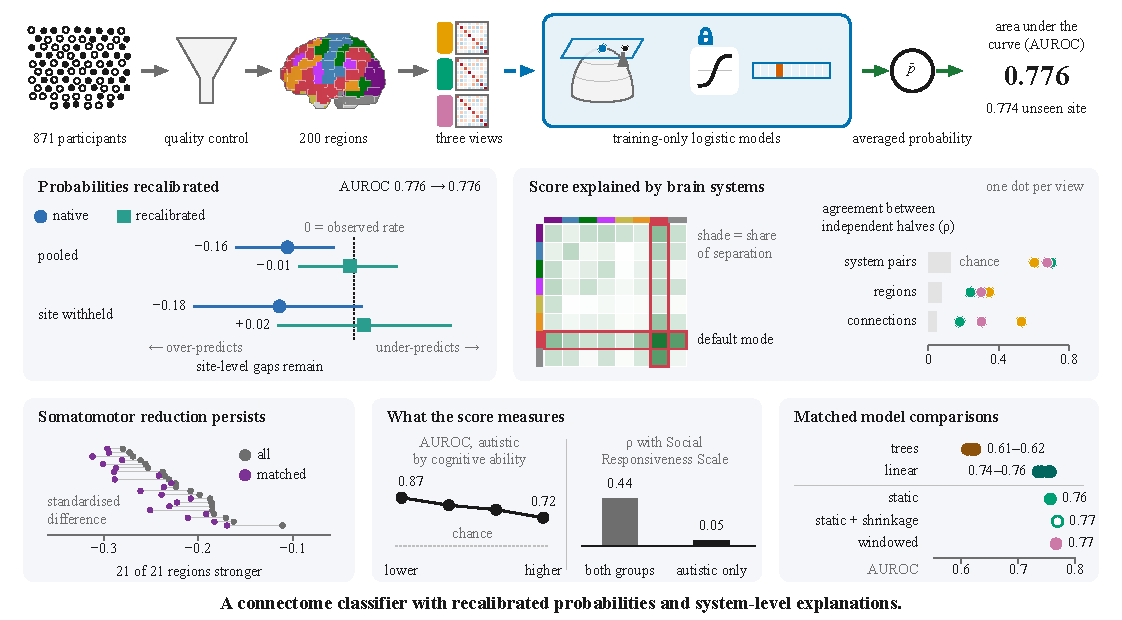
\includegraphics[width=\linewidth]{fig_graphical_abstract}
\end{graphicalabstract}

\begin{highlights}
\item Recalibration inside training folds restores calibration-in-the-large
\item Exact system-level attribution replicates across independent halves of the cohort
\item Somatomotor hypoconnectivity survives motion matching; default mode leads the score
\item Detection falls with IQ, and scores separate groups without tracking severity
\item Regularised linear models beat fixed trees; windowed gains reflect shrinkage
\end{highlights}

\begin{keywords}
Autism spectrum disorder \sep Functional connectome \sep Resting-state fMRI \sep Bioinformatics \sep Calibration \sep Interpretability
\end{keywords}

\maketitle   

\section{Introduction}
\label{sec:introduction}

% Part 1: the core problem
Autism spectrum disorder (ASD) is recognised as a neurodevelopmental condition in which social communication and behavioural patterns are affected \citep{Maenneretal2023}. ASD diagnosis is dependent on behavioural
assessment by trained clinicians, supported by the Autism Diagnostic Observation Schedule (ADOS-2)
\citep{CHOP_ADOS2} and the Autism Diagnostic Interview--Revised \citep{Lordetal1994}.
Each assessment is conducted in person by trained clinicians through behavioural observation and clinical judgement, making the diagnostic process both time- and resource-intensive. Timely access to assessment is therefore important, as earlier ASD identification enables appropriate interventions and support during critical stages of development, in line with current clinical recommendations \citep{Zwaigenbaumetal2015}. Brain-based measurements are therefore being investigated as research tools for characterising autism-related variation and for studying whether diagnostic groups can be distinguished from neuroimaging data.


Resting-state functional MRI (rs-fMRI) provides estimates of functional connectivity from spontaneous blood-oxygen-level-dependent activity across brain regions. These connectomes have been widely used for autism-related group comparisons and classification. These signals are then used to estimate functional connectivity, which is defined as the statistical relationship between the activity of different brain regions. In autistic individuals, differences in functional connectivity are observed across several brain regions and networks in large multisite studies. Functional connectivity therefore serves as an input for group comparisons and ASD classification. Large multisite resources such as the Autism Brain Imaging Data Exchange I (ABIDE-I) have enabled connectome-based autism classification to be studied across heterogeneous acquisition sites and participant populations. In ABIDE-I, rs-fMRI and phenotypic data from 1,112 participants across multiple sites are made openly available \citep{DiMartinoetal2014}. The dataset is based on a research population, in which participants are recruited for research studies and most individuals in the non-autistic group are typically developing controls.


% Part 2: the problem identified
A central problem in connectome-based autism classification is that measured performance and biological interpretation can be entangled with cohort composition, motion, feature construction, regularisation, and model design. ABIDE-I provides a suitable multisite setting in which these factors can be examined within the same analytical framework. Systematic reviews of ABIDE-I studies report differences in sample selection, preprocessing, validation methods, and classifier design, which limit direct comparison across studies \citep{Santanaetal2022,Hudaetal2024}. Participant composition is one important source of variation. Cognitive ability differs substantially across autistic participants, yet classification performance is usually reported only for the overall cohort. In published ABIDE-I benchmarks, classification performance is generally reported for the overall cohort, and performance across different levels of cognitive ability is rarely examined \citep{Heinsfeldetal2018,Eslamietal2019,AlmuqhimSaeed2021}. Full-scale intelligence quotient (IQ) varies across autistic participants and is generally lower than that of non-autistic participants in the dataset (Table~\ref{tab:participants}). Classification performance may therefore be affected by the cognitive characteristics of the participants included in the analysis. Variation in classifier scores with verbal IQ has also been reported in ABIDE data \citep{Nielsenetal2013}. This evidence is not sufficient to establish whether the relationship is specifically associated with autism. Head motion creates a related interpretive problem because it alters measured functional connectivity and differs between diagnostic groups \citep{Poweretal2012}. In this study, head motion is measured using mean framewise displacement, which represents the average movement of the head between consecutive image volumes. Greater head motion is observed among autistic participants in the dataset (Table~\ref{tab:participants}), indicating that reported functional-connectivity differences may also be affected by motion. This issue is relevant to reported reductions in connectivity within the somatomotor system, which includes regions involved in movement and bodily sensation \citep{Holigaetal2019,Ilioskaetal2023}. Only the linear effect of motion is removed through motion regression. It therefore remains unclear whether this connectivity difference is preserved when autistic and non-autistic participants are explicitly matched for head motion.

Model design provides a second source of uncertainty. Increasingly complex nonlinear classifiers are proposed for autism classification, but their apparent gains are difficult to isolate when feature representations, cohorts, and validation procedures also differ. More complex nonlinear models are increasingly proposed for ASD classification \citep{Liuetal2024MADE,Tangetal2025GNNLSTM,Tangetal2026CASGNN}. Strong performance with tangent-space connectivity and regularised linear classifiers is also reported in an earlier benchmark \citep{Dadietal2019}. Regularised linear classifiers on tangent-space connectivity remain strong baselines despite the increasing use of nonlinear models. The independent effect of classifier choice cannot be determined reliably from comparisons across existing studies because other parts of the analysis pipeline also differ. Its effect is therefore evaluated using the same participants, features, and cross-validation folds. Performance alone also does not establish what the classifier score represents. Associations with symptom severity may reflect diagnostic-group separation, while apparent gains from windowed connectivity may arise from the stronger covariance regularisation required for short windows. Classifier scores have been reported to correlate with symptom severity and have been interpreted as evidence of a graded phenotype \citep{Nielsenetal2013}. When this correlation is calculated across both diagnostic groups, much of the association may be produced by group separation because severity measures also differ between the groups. It is therefore not established that classifier scores vary with symptom severity within autistic participants. Second, the contribution of temporal information beyond static connectivity is examined. Windowed connectivity is proposed to represent changes in connectivity during a scan \citep{Hutchisonetal2013,Allenetal2014,Pretietal2017}. Covariance estimates from short windows are known to be unstable and require additional regularisation \citep{LeonardiVanDeVille2015}. Additional regularisation may therefore contribute to the apparent advantage of windowed connectivity. For a fair comparison, the same regularisation is therefore applied to the whole-scan representation.

Two further requirements concern the reliability of the fitted model itself: its probabilities should be calibrated, and its explanations should be reproducible. Hence, at first, the reliability of the probabilities returned by the ensemble is considered. Correct ranking of participants may be achieved even when predicted probabilities are systematically too high or too low. This property is not captured by the discrimination measures commonly reported in ABIDE-I benchmarks \citep{Guoetal2017,VanCalsteretal2019}. Second, the evidence used by the model is examined for interpretation at the level of brain systems. In a linear model, each connection weight is estimated together with all other connections and cannot be interpreted directly as a group difference \citep{Haufeetal2014}. Direct interpretation is made particularly unreliable when thousands of correlated connections are included. Both questions are therefore examined for the same ensemble to determine how reliably its scores and learned patterns can be interpreted.


% Part 3: existing solutions
Most connectome-based autism studies emphasise improvements in discrimination through alternative connectivity representations, deep models, graph methods, or site harmonisation. Comparatively less attention has been given to whether measured performance changes across participant subgroups, whether predicted probabilities are calibrated, and whether the patterns used to interpret a classifier reproduce in independent data. Different representations of functional connectivity, including the tangent-space projection of covariance matrices \citep{Varoquauxetal2010}, are compared in a controlled benchmark \citep{Dadietal2019}. Accuracies close to 0.70 are reported for deep autoencoder models on ABIDE-I \citep{Heinsfeldetal2018,Eslamietal2019,AlmuqhimSaeed2021}. Graph-based and convolutional models are also used to represent relationships between participants \citep{Parisotetal2018} and connections within brain networks \citep{Kawaharaetal2017}. These modelling approaches are further extended through multi-atlas deep ensembles \citep{Liuetal2024MADE}, dynamic graph models \citep{Tangetal2025GNNLSTM}, and multimodal graph models \citep{Tangetal2026CASGNN}. Differences between acquisition sites are addressed through harmonisation methods \citep{Johnsonetal2007,Fortinetal2018} and validation on held-out sites \citep{Abrahametal2017}. Performance in most of these studies is reported for the whole cohort, so variation in classification performance across participant groups is not clearly established. It also remains unclear whether reported differences in functional connectivity are preserved when head motion is directly controlled. In addition, the effect of classifier family is rarely examined under the same cross-validation setting, apart from the controlled benchmark reported \citep{Dadietal2019}. Together, these limitations motivate a controlled analytical framework in which the same connectome pipeline is used to separate the effects of participant composition, measurement confounding, modelling choices, probability calibration, and explanation stability.

% Part 4: what is proposed
To isolate these sources of variation, a fixed connectome-classification pipeline is used as an experimental framework rather than as the primary object of comparison. In this pipeline, three connectivity
descriptions are computed for each participant: correlation, static tangent-space, and
windowed tangent-space connectivity. The windowed description is computed from shorter
segments, or windows, of each scan. Correlation, static tangent-space, and windowed tangent-space connectivity are analysed within a common regularised linear framework and evaluated under pooled and site-held-out validation.  Performance is estimated under two schemes. In pooled ten-fold
validation, participants from all sites are divided into ten folds; in leave-one-site-out validation, each of the 20 recorded site labels is held out once. Discrimination is summarised by the area under the receiver operating characteristic curve (AUROC). Participant-pooled values are computed once from all held-out predictions, whereas fold-mean values are averaged across folds. The framework is then used to determine how participant characteristics and motion affect measured discrimination and connectivity differences, how modelling and regularisation choices alter performance, and whether classifier probabilities and explanations can be interpreted reliably. The group contrasts are conducted as univariate analyses independently of the classifier. These analyses and the cognitive-ability analysis are treated as exploratory and are performed without global signal regression, under which the whole-brain mean signal would be removed (Sections~\ref{subsubsec:data-preprocessing} and~\ref{subsec:group-differences}). The selection-scope, symptom-association, shrinkage-control, and recalibration analyses are designated as primary descriptive comparisons. The classifier comparison is designated as secondary. Score attribution and the reproducibility of its pattern are also designated as secondary analyses because they are added after the primary discrimination results are examined. The evidential weight of each result is defined by these designations (Section~\ref{subsubsec:analysis-status}).

From this framework, five findings are developed concerning probability calibration, reproducible model interpretation, motion-matched connectivity differences, the meaning of classifier scores across cognitive and symptom dimensions, and the effects of model complexity and covariance regularisation. The analyses supporting each contribution are reported in Section~\ref{sec:results}.

\begin{itemize}

\item \textbf{Training-only calibration of connectome-classifier probabilities.} Cross-fitted recalibration within the training partition removes the average probability offset without changing discrimination. Calibration-in-the-large is improved from $-0.162$ to $-0.010$ without changing the AUROC, and the offset is traced to the penalised solver intercept. The effect on threshold-based decisions is also quantified, with sensitivity changing from 0.705 to 0.655 at a threshold of 0.5 and residual site-level miscalibration being identified.

\item \textbf{Reproducibility of connectome-classifier interpretation across biological scales.} The ensemble score is divided exactly among 36 functional-system pairs, and the resulting attribution is tested on independent cohort halves against a permutation reference. High agreement is also obtained from overlapping training partitions with permuted diagnoses, reaching 0.88 for individual connections compared with 0.91--0.95 for the real labels. Greater reproducibility is obtained at the system level, with Spearman correlations of 0.60--0.70, while weaker agreement is obtained for individual connections at 0.18--0.53. Interpretation at the functional-system level is therefore more strongly supported than interpretation of individual connections.

\item \textbf{Motion-matched evidence for somatomotor connectivity differences and system-level classifier attribution.} Evidence is obtained from both nuisance-adjusted group analysis and classifier attribution. The somatomotor reduction increases from $-0.215$ to $-0.249$ after participants are matched for head motion. In the classifier, the largest share of group separation is assigned to default-mode pairs, and the greatest contribution per connection is obtained from the somatomotor system. Agreement with the regional group-difference pattern is also observed within the somatomotor system, with Spearman correlations of 0.78--0.93. These findings are treated as exploratory associations and are not interpreted as evidence of a biomarker.

\item \textbf{Characterisation of what a connectivity-based autism score reflects across cognitive ability and symptom severity.} Lower discrimination is observed as full-scale IQ increases among autistic participants, with AUROC decreasing from 0.873 to 0.719. Diagnostic-group separation is captured by the classifier score, and little association with symptom severity is observed within autistic participants, with Spearman correlations of 0.438 across both groups and 0.050 within the autistic group. The score is therefore supported as a measure of group separation rather than symptom severity, and its performance is interpreted within the cognitive range of the evaluated sample.

\item \textbf{Matched evidence on the effects of classifier choice and covariance regularisation in connectome models.} Identical features and cross-validation folds are used for the classifier comparison, under which higher AUROC is obtained with regularised linear models (0.735--0.757) than with fixed-configuration tree ensembles (0.611--0.624). The apparent advantage of windowed connectivity is removed when the same covariance shrinkage is applied to the whole-scan representation, leaving a difference of $-0.002$. These results support regularised tangent-space connectivity as a strong baseline for comparisons with more complex models and representations.

\end{itemize}
The remainder of the paper is organised as follows: related work is reviewed in
Section~\ref{sec:related}, the methods are described in
Section~\ref{sec:methods}, and the results are reported in Section~\ref{sec:results}.
The findings are then discussed in Section~\ref{sec:discussion}, and conclusions are drawn in
Section~\ref{sec:conclusion}.

\section{Related Work}
\label{sec:related}

Research on autism spectrum disorder (ASD) classification using resting-state functional magnetic resonance imaging (rs-fMRI) has gradually developed from statistical modelling and functional-connectivity representation. More recent research is focused on multisite learning, deep architectures, dynamic connectivity, multimodal fusion, and reliability-aware prediction. In early studies, methods are established for representing high-dimensional covariance and brain-network information. These methods are later extended through deep learning, multiple brain atlases, temporal modelling, and graph-based approaches to improve classification performance. Alongside these developments, calibration, interpretability, selective prediction, and statistical validation are increasingly used to improve the reliability of machine-learning predictions. Overall, the performance and reliability of ASD classification are shaped by several methodological choices, including how functional connectivity is represented, how variation across acquisition sites is controlled, and how prediction uncertainty is assessed.

\subsection{Foundations of Functional Connectome-Based Analysis}


The methodological basis for connectome-based ASD classification is established through a sequence of statistical and neuroimaging developments. Reliable evaluation first requires uncertainty in classification error to be quantified, for which exact confidence limits for binomial outcomes are provided. Reliable connectivity estimation is then required before such models can be evaluated. High-dimensional covariance estimation is stabilised through the Ledoit--Wolf shrinkage method \citep{LedoitWolf2004}, which is particularly relevant to rs-fMRI because many regional signals are estimated from limited time points. Once stable features are obtained, reliable comparison between classifiers is supported by statistical procedures for model evaluation. The use of multisite data introduces an additional source of variation, which is addressed through the ComBat empirical-Bayes framework for batch-effect correction \citep{Johnsonetal2007} and its later adaptation to neuroimaging for scanner- and site-related harmonisation \citep{Fortinetal2018}. With these statistical foundations in place, the structure of connectivity itself is modelled more directly. Covariance matrices are represented according to their non-Euclidean geometry \citep{Varoquauxetal2010}, from which tangent-space representations are established for functional-connectivity analysis. Biological interpretation is then supported by the identification of seven large-scale intrinsic brain networks \citep{Yeoetal2011}, through which individual connections are interpreted within broader functional systems. Connectivity is first represented statically across the full scan, after which temporal variation is examined through dynamic functional connectivity \citep{Hutchisonetal2013}. Functional connectivity is therefore developed from stable covariance estimation toward geometrically informed, biologically organised, and temporally resolved representations.

\subsection{Multisite ASD Data and Reproducibility}

Large-scale ASD neuroimaging research is substantially advanced through the release of ABIDE \citep{DiMartinoetal2014}. Data from multiple international sites are combined, making larger ASD classification studies possible. This increased scale also introduces variation in scanner type, acquisition protocol, demographic composition, and site characteristics. As a result, prediction models risk capturing acquisition-related differences instead of ASD-related neural patterns. The use of larger multisite datasets also requires high-dimensional brain information to be represented carefully. Regularised matrix regression is proposed for this purpose, where predictors are kept in matrix form so that relationships among features are preserved during modelling \citep{ZhouLi2014}. Careful analysis is also required when changes in connectivity over time are examined. Sliding-window estimates are shown to depend on window length, and apparent connectivity changes are potentially produced by analysis choices \citep{LeonardiVanDeVille2015}. Temporal information therefore needs to be evaluated with careful control of scan length and window design. These methodological choices directly affect whether findings are reproducible across datasets and sites. Using multisite resting-state data, biomarker performance is shown to depend on preprocessing, feature construction, and validation design \citep{Abrahametal2017}. The reliability of time-varying connectivity is also examined through a review of dynamic functional-connectivity methods \citep{Pretietal2017}. Together, these studies show that stable ASD-related findings depend on careful control of participants, analysis choices, and acquisition sites.

\subsection{Reliability, Calibration, and Explainability}

Alongside developments in neuroimaging representation and generalisation, reliability-oriented machine-learning methods are also developed. Probability calibration is examined in a study \citep{Guoetal2017}, where high classification accuracy is shown to be insufficient for reliable probability estimates. Participants may be ranked correctly even when the predicted probabilities do not match observed outcome frequencies. Calibration is therefore assessed through calibration-in-the-large, calibration slope, and the Brier score. Systematic probability offsets can be corrected through recalibration fitted on data separate from the evaluation set \citep{VanCalsteretal2019,Steyerbergetal2010,ZadroznyElkan2002}. Selective classification is introduced in a study \citep{GeifmanElYaniv2017}, where uncertain cases are allowed to remain unclassified instead of requiring a prediction for every input. Prediction error can therefore be reduced at the cost of lower coverage, which is relevant to screening settings where uncertain cases are referred for further clinical assessment. Model interpretation is also considered at both the individual-prediction and feature-pattern levels. Contributions to individual predictions are quantified through SHAP \citep{LundbergLee2017}. For linear models, model weights are not interpreted directly as differences between groups, and a corresponding pattern relating each feature to the model output is required \citep{Haufeetal2014}. Evaluation is consequently extended beyond discrimination: calibration is used to assess probability reliability, selective prediction is used to define when a prediction is issued, and explanation methods are used to identify the information contributing to model output. Clinical usefulness is assessed separately through decision-curve analysis \citep{VanCalsteretal2018}. Reliable ASD classification is therefore evaluated through discrimination, calibration, selective decision-making, interpretability, and clinical usefulness.



\subsection{Deep Learning for ASD Classification}

Alongside these reliability-focused developments, deep learning is increasingly applied to ABIDE functional-connectivity data. Distributed connectivity patterns are learned automatically and an accuracy of approximately 70.0\% is reported, showing that ASD-related information is captured through deep feature learning \citep{Heinsfeldetal2018}. The effect of multisite variation still needs to be addressed when such models are applied to ABIDE. For this purpose, ComBat is adapted for neuroimaging harmonisation in a study \citep{Fortinetal2018}, allowing scanner- and site-related variation to be reduced while biological variation is preserved. The harmonisation step also needs to be estimated without information from held-out test data. Deep representation learning is further developed through ASD-DiagNet, which is proposed in a study \citep{Eslamietal2019}. Representation learning and classification are combined, and an accuracy of approximately 70.3\% is reported. The small difference in performance indicates that classification is also potentially influenced by the way functional connectivity is represented. This role of connectivity representation is examined more directly in a controlled benchmarking study \citep{Dadietal2019}. Multiple connectome representations and predictive models are compared under the same setting, and tangent-space connectivity is identified as a strong representation. With an appropriate connectivity representation, comparatively simple classifiers are shown to remain competitive with more complex nonlinear models. Sparse representation learning is further explored through ASD-SAENet, which is proposed in a study \citep{AlmuqhimSaeed2021}. A sparse autoencoder is combined with a deep neural network, and an accuracy of approximately 70.8\% is reported. Across these deep-learning approaches, the increase from 70.0\% to 70.3\% and then 70.8\% remains relatively small. This pattern suggests that deeper representation learning alone does not necessarily fully address the challenges of heterogeneous multisite rs-fMRI data.


\subsection{Evidence from Systematic Reviews}

The broader performance of rs-fMRI machine-learning methods is examined through a systematic review and meta-analysis in \cite{Santanaetal2022}. Moderate pooled sensitivity, specificity, and discrimination are reported, while considerable methodological heterogeneity is identified. Differences in preprocessing, sample selection, validation strategy, feature extraction, and classifier design make direct comparison between studies difficult. A later systematic review of deep-learning and rs-fMRI biomarkers \cite{Hudaetal2024} reports continued methodological development but identifies similar limitations related to generalisability, reproducibility, and inconsistent evaluation. These reviews provide an important analytical perspective: higher accuracy reported by an individual model cannot be interpreted independently of the dataset definition and experimental pipeline used to obtain it. Therefore, later ASD classification studies increasingly attempt to improve the representation itself rather than only increasing classifier depth.

\subsection{Multi-Atlas and Dynamic Connectivity Models}

Dependence on a single brain parcellation is addressed through MADE-for-ASD \cite{Liuetal2024MADE}. A multi-atlas deep ensemble is introduced, and approximately 75.2\% accuracy is reported. Different atlases describe the same brain according to different regional boundaries, so their predictions potentially contain complementary information. Multi-atlas fusion therefore provides a possible way to reduce dependence on one predefined parcellation. However, the improvement is introduced together with a more complex ensemble architecture. It therefore becomes difficult to determine whether performance is improved because of atlas diversity, deep-model capacity, demographic information, or their interaction. This motivates controlled evaluations in which atlas fusion is varied while the remaining pipeline is kept unchanged. Dynamic functional connectivity is later revisited through a GNN-LSTM framework \cite{Tangetal2025GNNLSTM}. Graph neural networks are combined with temporal sequence modelling, and approximately 80.4\% accuracy is reported on ABIDE-I. Compared with static approaches, connectivity variation across the scan is explicitly represented rather than being averaged into one matrix. This development addresses an important limitation of static functional connectivity, but it introduces several additional decisions. Window length, overlap, temporal ordering, graph construction, and sequence-model complexity all affect performance. Therefore, the contribution of temporal variation requires separation from the contribution of the classifier through controlled ablation.

\subsection{Explainable and Multimodal ASD Models}

Interpretability receives greater attention in recent ASD classification research. Explainable artificial intelligence is applied to ABIDE fMRI data in a study \cite{Vidyaetal2025}, where highly predictive performance is reported under the stated filtering condition and influential brain regions are identified through multiple explanation methods. Such work demonstrates the potential of connecting prediction with biologically interpretable patterns. However, unusually high performance on heterogeneous multisite data also increases the importance of strict validation. Feature selection, filtering, preprocessing, and cross-validation are required to remain independent of held-out data. The broader lesson from earlier benchmarking \cite{Dadietal2019} and meta-analysis \cite{Santanaetal2022} therefore remains relevant: reported performance requires interpretation together with the complete experimental procedure. The progression toward richer representations continues through CAS-GNN \cite{Tangetal2026CASGNN}. Structural and functional MRI are integrated using cross-attention and subject-adaptive graph construction, and approximately 79.3\% accuracy is reported. Compared with earlier functional-connectivity-only approaches, multimodal information is used to represent each participant more comprehensively. Although multimodal graph learning increases representational capacity, additional learned components also make generalisation more difficult to assess. Performance gains therefore require evaluation against cross-site stability, model complexity, and potential overfitting.

\subsection{Research Gap}

Two connected methodological developments are identified in the literature. In the first, functional connectivity is progressively represented through stable covariance estimation \cite{LedoitWolf2004}, geometric modelling \cite{Varoquauxetal2010}, network-level organisation \cite{Yeoetal2011}, and dynamic connectivity \cite{Hutchisonetal2013,LeonardiVanDeVille2015,Pretietal2017}. These representations are extended to multisite analysis \cite{DiMartinoetal2014}, reproducibility assessment \cite{Abrahametal2017}, deep learning \cite{Heinsfeldetal2018,Eslamietal2019,AlmuqhimSaeed2021}, multi-atlas fusion \cite{Liuetal2024MADE}, dynamic graph modelling \cite{Tangetal2025GNNLSTM}, and multimodal graph learning \cite{Tangetal2026CASGNN}. Increasingly rich representations are therefore introduced, together with additional sources of variation and overfitting that require controlled evaluation. In the second development, greater attention is given to prediction reliability.Confidence estimation and statistical comparison are formalised and reliability is further addressed through harmonisation \cite{Johnsonetal2007,Fortinetal2018}, calibration \cite{Guoetal2017}, selective prediction \cite{GeifmanElYaniv2017}, explainability \cite{LundbergLee2017}, and decision-oriented evaluation \cite{VanCalsteretal2018}. Classification accuracy alone is therefore insufficient for screening-oriented use; reliable probabilities, uncertainty-aware decisions, interpretable evidence, and performance across unseen sites are also required. These methodological directions are commonly evaluated separately, leaving dynamic connectivity, multi-atlas information, harmonisation, interpretability, calibration, selective prediction, and cross-site generalisation without a common controlled evaluation. The benefit of increasingly complex classifiers over carefully designed functional-connectivity representations also remains uncertain when identical validation conditions are imposed. The present work is therefore structured as a controlled, reliability-oriented evaluation. Complementary functional-connectivity representations are compared using the same data partitions, tangent-space quantities are estimated from training data only, and cross-site performance is assessed through leave-one-site-out validation. Ensemble probabilities are assessed for calibration and are recalibrated within the training partitions when systematic offset is identified. The ensemble score is also attributed exactly to functional-system pairs, and the reproducibility of this attribution is tested against a permutation reference. Each component is evaluated independently so that observed improvements are attributed to the corresponding methodological choice rather than to model complexity alone.


\section{Methods}
\label{sec:methods}

The methodology follows a unified pipeline from participant selection to model evaluation and statistical analysis (Figure~\ref{fig:overview}). A primary cohort of 871 participants is selected from ABIDE-I using the available anatomical and functional image-quality ratings. Preprocessed regional time series are obtained from the C-PAC \texttt{filt\_noglobal} derivative using the CC200 atlas and are used to construct three functional-connectivity representations: whole-scan correlation, static tangent-space connectivity, and windowed tangent-space connectivity. Each representation is modelled separately using $\ell_2$-regularised logistic regression, and the resulting probabilities are averaged to form the primary ensemble. Model performance is evaluated using pooled ten-fold cross-validation and leave-one-site-out validation, with regularisation selected within the corresponding training partitions. All data-dependent transformations, including tangent-space references and feature scaling, are estimated from training data before being applied to held-out participants. The resulting out-of-fold predictions form the basis for assessing discrimination, calibration, recalibration, and threshold-based behaviour. Additional analyses examine how participant characteristics, head motion, feature selection, classifier choice, connectivity representation, cohort definition, and other analytical decisions influence the reported results. Functional-connectivity group differences are evaluated separately with nuisance adjustment and motion-matched sensitivity analyses. The linear ensemble members are also examined at the level of functional systems to determine which patterns contribute to classifier scores and how reproducibly these patterns are recovered. Together, these analyses are designed to evaluate not only predictive performance, but also the conditions under which the resulting probabilities, connectivity findings, and model interpretations can be considered reliable.

\begin{figure}[pos=htbp]
\centering
\includegraphics[width=\linewidth,height=0.84\textheight,keepaspectratio]{fig_overview}
\caption{Overview of the primary analysis pipeline. (a) ABIDE-I participants are screened by image-quality control (QC), and CC200 regional time series are extracted from preprocessed rs-fMRI data. Regions are coloured by functional system: VIS, SMN, DAN, SAL, LIM, FPN, DMN, and SUB. (b) Shrinkage-based correlation, static tangent-space connectivity, and windowed tangent-space connectivity are derived, with tangent references estimated from the training partition only. (c) Each representation is vectorised, standardised using training-derived statistics, and classified by $\ell_2$-regularised logistic regression with inner three-fold CV. Model probabilities are averaged for the final ensemble, which is evaluated using pooled ten-fold and LOSO CV. Circled numbers mark \ding{202}~QC, \ding{203}~time series and windows, \ding{204}~scaling, \ding{205}~logistic regression with tuning, and \ding{206}~probability averaging at the 0.5 threshold. Locked blue boxes indicate training-only estimates; grey arrows show data flow, dashed blue arrows show fitted quantities applied unchanged, and dashed orange arrows indicate held-out-label leakage, which is absent from the pipeline.}

\label{fig:overview}
\end{figure}

The Methods are organised into ten subsections that follow the analysis pipeline. Section~\ref{subsec:study-design-cohort} describes the study design, data, cohorts, phenotypic variables, atlas, and scan-quality characteristics. Sections~\ref{subsec:connectivity-representations}--\ref{subsec:interpretation} define the connectivity representations, prediction model, validation strategy, probability-based analyses, and interpretation of the linear models. Planned comparisons and exploratory group-contrast analyses are described in Sections~\ref{subsec:planned-comparisons} and~\ref{subsec:group-differences}, followed by the statistical analysis in Section~\ref{subsec:statistical-analysis}. Reproducibility and the scope of the resulting estimates are addressed in Section~\ref{subsec:reproducibility-scope}.


\subsection{Study design and cohort}
\label{subsec:study-design-cohort}

This subsection defines the study question, the data, and the participant cohorts on which
the analyses are based. These definitions are given first, because all representations,
models, and comparisons are based on these data and cohorts. The study design is
described in Section~\ref{subsubsec:study-design}, and the data source and preprocessing in
Section~\ref{subsubsec:data-preprocessing}. The primary cohort is then defined in
Section~\ref{subsubsec:cohorts}, and the wider QC cohort in Section~\ref{subsubsec:cohorts}.
Next, the phenotypic variables and the handling of missing values are specified in
Section~\ref{subsubsec:phenotypic-variables}. The atlas and the signal-quality procedure are described in
Section~\ref{subsubsec:atlas-signal-quality}. Finally, the treatment of differences in scan length is described
in Section~\ref{subsubsec:scan-length}.

\subsubsection{Study design}
\label{subsubsec:study-design}

Clinical diagnosis of ASD combines direct observation,
developmental history, and professional judgement. In this study, ASD status is defined by
the diagnostic labels provided in ABIDE-I, while
rs-fMRI is used to characterise
large-scale functional connectivity in autistic and non-autistic participants. The ASD classification target is derived directly from the ABIDE-I diagnostic labels. Participants with \texttt{DX\_GROUP = 1} are coded as autistic, whereas those with
\texttt{DX\_GROUP = 2} are coded as non-autistic. The primary analysis therefore evaluates
how well the imaging-based models distinguish autistic from non-autistic participants within
the ABIDE-I research cohort.

Discrimination is evaluated primarily using participant-pooled out-of-fold AUROC under pooled ten-fold and
LOSO validation. For each participant, the prediction used for evaluation is
generated by a model fitted without that participant's held-out data, and predictions from
all held-out folds are subsequently combined to calculate the overall AUROC. AUROC is used
as the primary discrimination measure because it assesses the ranking of autistic and
non-autistic participants across prediction scores without requiring a fixed classification
threshold. In pooled ten-fold validation, participants from all sites are distributed across ten folds,
with each fold held out once, providing an estimate of generalisation within the combined
ABIDE-I multisite cohort. LOSO validation instead holds out all participants
associated with one site label at a time, providing a more stringent assessment of
generalisation to an ABIDE-I site that is absent from model training.

The primary prediction model is defined as an equal-weight ensemble of three connectivity representations. Six comparative analyses and two ensemble-level analyses are used to examine the main methodological questions of the study. In four comparative analyses, discrimination across cognitive-ability groups, the persistence of functional-connectivity differences after within-site matching for head motion, the effect of feature-selection scope and granularity, and the performance of different classifier families under the same representation and validation procedure are assessed. In the remaining two, symptom associations and the windowed connectivity description are examined. Classifier-score associations are assessed both across the full cohort and within autistic participants. For windowed connectivity, the same covariance shrinkage is applied to the whole-scan description so that regularisation is matched between the two representations. The ensemble itself is then examined through probability calibration and score attribution. Ensemble probabilities are assessed and recalibrated within the training partitions when systematic offset is identified, and the ensemble score is attributed to functional-system pairs whose reproducibility is tested against a permutation reference. The cognitive-subgroup, head-motion matching, feature-selection, and classifier-comparison procedures are integrated with the validation design in Section~\ref{subsubsec:outer-validation}.


\subsubsection{Data source and preprocessing}
\label{subsubsec:data-preprocessing}

Data are obtained from ABIDE-I, a multi-site research dataset that combines rs-fMRI, anatomical magnetic resonance imaging, and phenotypic information from 1,112 participants across 17 acquisition sites \citep{DiMartinoetal2014}. The phenotypic records provide diagnostic status together with demographic and cognitive measures, including age, sex, full-scale IQ, verbal IQ, performance IQ, handedness, and acquisition site. These variables are retained to characterise the study population and to support the subgroup and covariate analyses described later. After the QC procedure described in Section~\ref{subsubsec:cohorts}, the primary cohort contains 871 participants, including 403 autistic and 468 non-autistic participants. The cohort includes 727 male and 144 female participants and spans 6.5--58 years of age, with a mean age of 16.9 years (standard deviation [SD] 7.6). Mean full-scale IQ is 105.8 in the autistic group and 111.1 in the non-autistic group. Because ABIDE-I combines data acquired independently at multiple centres, heterogeneity remains across sites in scanner hardware, acquisition protocols, scan duration, participant composition, and image quality \citep{Abrahametal2017}. Image quality is therefore considered explicitly during cohort selection using the anatomical and functional quality ratings provided with the release. Preprocessed imaging outputs are obtained from the Preprocessed Connectomes Project \citep{Craddocketal2013}, which provides ABIDE-I data processed through standardised workflows and thereby supports consistent preprocessing across participants from different acquisition sites. The use of these publicly released derivatives also improves reproducibility by fixing the imaging inputs and preprocessing choices. The present study uses outputs generated with C-PAC, specifically the \texttt{filt\_noglobal} processing strategy.

Within the selected C-PAC workflow, temporal and spatial sources of unwanted variation are addressed before functional connectivity is estimated. Slice-acquisition timing differences are corrected, successive functional volumes are realigned to reduce motion-related displacement, non-brain tissue is removed, signal intensities are normalised, and the functional images are aligned with the corresponding anatomical images. Additional variation associated with head motion and non-neural signals is reduced through nuisance regression using a 24-parameter motion model, five CompCor components derived from white-matter and cerebrospinal-fluid signals, and linear and quadratic temporal trends. This processing reduces contributions from residual head motion, physiological noise, and slow signal drift before connectivity is calculated. The resulting signals are then band-pass filtered between 0.01 and 0.10~Hz to retain the low-frequency fluctuations used for resting-state functional-connectivity analysis, while global signal regression is not applied under the selected \texttt{filt\_noglobal} strategy \citep{Craddocketal2013}. Following preprocessing, the functional data are reduced from voxel-level images to atlas-defined regional time series. For the primary analysis, the CC200 atlas divides the brain into 200 functionally defined regions, and the signal within each region is summarised across the scan to produce one time series per region and participant. These 200 regional time series form the common imaging input from which the correlation, static tangent-space, and windowed tangent-space connectivity representations are constructed. Although the common C-PAC workflow reduces variation caused by inconsistent preprocessing procedures, heterogeneity arising from acquisition conditions and participant composition remains part of the ABIDE-I multisite setting. These remaining sources of variation are addressed through QC-based cohort selection, site-aware validation, nuisance adjustment, and the sensitivity analyses described in the following sections.

\subsubsection{Primary and wider quality-control cohorts}
\label{subsubsec:cohorts}

The analysis cohorts are defined using the anatomical and functional image-quality ratings
provided with ABIDE-I. These ratings identify whether the available scans are suitable for
analysis and are accompanied by annotations for issues such as excessive head motion,
unsuccessful skull stripping, incomplete or distorted anatomical coverage, preprocessing
failure, image noise, missing imaging modalities, and regional signal dropout. For the
primary cohort, a participant is retained only when the required assessment from all three
raters is satisfied: rater~1 is required to mark the scan as acceptable; rater~2 is required to rate both the
anatomical and functional images as acceptable or borderline; and rater~3 is required to rate both
images as acceptable. Applying this criterion excludes 241 of the 1,112 ABIDE-I records.
Because the quality annotations sometimes overlap, an excluded scan is potentially associated with more
than one recorded issue. The resulting primary cohort contains 871 participants, including
403 autistic and 468 non-autistic participants. It comprises 727 male and 144 female
participants, with ages ranging from 6.5 to 58 years (mean 16.9 years; median 14.8 years).
Cohort membership is fixed before the primary analyses, and participant identifiers are
cross-checked against the phenotypic records to ensure that the same participants are used
throughout the prediction pipeline. The cohort-selection procedure and subsequent
time-series extraction are summarised in Figure~\ref{fig:overview}a.

Participant characteristics by diagnostic group are reported in
Table~\ref{tab:participants}. Welch's $t$-test is used to compare age and the three IQ measures---full-scale, verbal, and performance---between the
autistic and non-autistic groups, allowing for unequal group variances. Mean FD, defined in Section~\ref{subsubsec:phenotypic-variables}, is examined using both Welch's
$t$-test and the Mann--Whitney $U$ test. The former compares group means, whereas the latter
provides a rank-based comparison that is less sensitive to the right-skewed FD
distribution. Scan length is compared using the Mann--Whitney $U$ test, and sex
distributions are compared using the $\chi^2$ test with Yates' continuity correction.
Because cognitive ability and head motion potentially influence subsequent results, their effects
are examined separately in the cognitive-subgroup analysis of
Section~\ref{par:cognitive-sex-subgroups} and the motion-matched group-contrast analysis of
Section~\ref{subsubsec:system-motion-regional}.

A wider QC cohort is additionally defined to test whether the findings depend
on the more restrictive primary inclusion rule and to support comparison with previous ABIDE-I
studies. For this cohort, eligibility requires an acceptable functional-image rating from
rater~3, without applying the full three-rater criterion used for the primary cohort. This
definition identifies 1,035 eligible participants in the phenotypic records, of whom 1,032
have regional time series available for analysis. The 1,035-participant eligibility count
matches the cohort definition reported by \citet{Heinsfeldetal2018},
\citet{Eslamietal2019}, and \citet{AlmuqhimSaeed2021}. The wider cohort is therefore used
as a cohort-definition sensitivity analysis, allowing the primary results to be assessed
under a less restrictive QC rule while also providing a direct basis for
comparison with these previous reports.

\begin{table}[t]
\centering
\caption{Participant characteristics in the primary cohort (871 participants; 20 site labels from 17 acquisition sites). Values are mean (SD) or median [IQR]; available sample sizes are given in brackets when below the group total.}
\label{tab:participants}
\small
\begin{tabular}{@{}>{\raggedright\arraybackslash}p{0.36\linewidth}ccc@{}}
\toprule
Characteristic & Autistic (n = 403) & Non-autistic (n = 468) & p \\
\midrule
Age, years & 17.07 (7.96) & 16.84 (7.24) & 0.66 \\
Female, n (\%) & 54 (13.4) & 90 (19.2) & 0.027 \\
Full-scale IQ & 105.79 (17.06) [376] & 111.09 (12.08) [435] & $6.2\times10^{-7}$ \\
Verbal IQ & 104.89 (18.10) [342] & 111.57 (13.07) [379] & $2.8\times10^{-8}$ \\
Performance IQ & 105.69 (17.26) [344] & 107.91 (13.05) [391] & 0.052 \\
Mean FD (Section~\ref{subsubsec:phenotypic-variables}), mm & 0.126 (0.143) & 0.094 (0.082) & $8.2\times10^{-5}$ \\
Mean FD (Section~\ref{subsubsec:phenotypic-variables}), mm, median [IQR] & 0.088 [0.057, 0.144] & 0.068 [0.045, 0.109] & $8.9\times10^{-7}$ \\
Volumes per scan, median [range] & 176 [78, 316] & 176 [78, 316] & 0.77 \\
\bottomrule
\end{tabular}

\vspace{4pt}
\begin{minipage}{\linewidth}\footnotesize
p-values are from Welch's t-test for rows summarised by mean (SD), the Mann--Whitney U
test for rows summarised by median, and the $\chi^2$ test with Yates' continuity
correction for sex.
\end{minipage}
\end{table}

\subsubsection{Phenotypic variables}
\label{subsubsec:phenotypic-variables}

Phenotypic information is linked to each participant through the ABIDE-I identifiers and
includes age, sex, full-scale IQ, verbal IQ, performance IQ, handedness, and acquisition
site. These variables are used to characterise the cohort and to support the secondary,
subgroup, and nuisance-adjustment analyses described later. The primary ensemble itself is
restricted to imaging-derived connectivity features, so demographic and cognitive variables
do not contribute directly to its predictions. A separate phenotype model, described in
Section~\ref{par:phenotype-model}, instead uses age, sex, the three IQ measures, and handedness to
evaluate discrimination from non-imaging information. Acquisition site is retained for
site-based validation, nuisance adjustment, and sensitivity analyses. Head motion is represented separately by mean FD, obtained from
the \texttt{func\_mean\_fd} mean-FD quality metric provided with the preprocessed release. This
measure follows Jenkinson's formulation and is calculated from the rigid-body realignment
parameters between successive functional volumes, with rotational components converted to
millimetres using an 80-mm head radius. The resulting mean FD
provides a single scan-level summary of head motion for each participant and is used in the
participant-characteristic comparisons and the subsequent motion-adjusted and
motion-matched analyses.

Missing phenotypic entries are identified before analysis, including values recorded as
\texttt{-9999} or left blank. When phenotypic variables are used in predictive or
harmonisation models, missing continuous values are replaced by the median calculated from
the corresponding outer training partition. This prevents information from held-out
participants from entering preprocessing. The same rule is used for the secondary
phenotype model in Section~\ref{par:phenotype-model} and for age in the ComBat analysis of
Section~\ref{par:combat-harmonisation}. In the ComBat model, sex is coded as 0 for male and 1 for female.
No age or sex values are missing in the primary cohort. For analyses fitted directly to a complete analysis cohort, required missing covariates are
median-imputed from that cohort. This applies to the nuisance-adjustment procedures in
Sections~\ref{par:selection-scope} and~\ref{subsubsec:connection-adjustment}, as well as to the preparation for motion
matching in Section~\ref{subsubsec:system-motion-regional}. In contrast, no imputation is applied in the
symptom-association, cognitive-subgroup, instrument-concordance, component--symptom, or
participant-characteristic analyses. Participants with missing values are excluded only
from the analysis that requires the corresponding variable.

\subsubsection{Atlas and signal quality}
\label{subsubsec:atlas-signal-quality}

The primary analyses use the CC200 functional parcellation~\citep{Craddocketal2012}. All 200 regions are retained for prediction, yielding 19,900 unique pairwise connectivity features. A separate signal-quality check is applied before the group difference analyses because Pearson correlation cannot be computed for a region with no temporal variation. First, any region with a temporal SD of zero in more than 1\% of the 1,032 available CC200 time-series files is removed; four regions meet this criterion. Participants in the primary cohort are then excluded from the group-contrast analysis if any of the remaining regions contains a constant signal. This produces a group-contrast cohort of 863 participants and 196 regions, corresponding to 19,110 unique connections. To support system-level interpretation, each CC200 region is also assigned an anatomical label and a functional-system label. Yeo's seven cortical systems are mapped onto the CC200 space using nearest-neighbour interpolation~\citep{Yeoetal2011}, preserving a single system label for each voxel. Each region is assigned to the system with the greatest spatial overlap when that system covers more than 20\% of the region; regions that do not meet this threshold are assigned to a subcortical/cerebellar category. This procedure yields eight functional-system classes and 36 unique within- and between-system combinations, which are used to summarise connection-level group effects at the system level.

\subsubsection{Scan length}
\label{subsubsec:scan-length}

Scan length is considered explicitly in the dynamic-connectivity analyses because the number of available volumes differs substantially across participants and sites. In the primary cohort, scans contain between 78 and 316 volumes, with scan duration varying systematically by acquisition site. To keep the dynamic representations comparable, each participant contributes the same number of temporal windows regardless of total scan length. This prevents participants with longer scans from contributing more window-level estimates than those with shorter scans. Window length and temporal change are expressed in volumes rather than seconds because a harmonised repetition-time field is not available across the analysis files.

\subsection{Connectivity representations}
\label{subsec:connectivity-representations}

This subsection describes how each participant's regional rs-fMRI time series are
transformed into the three connectivity representations used by the primary ensemble:
shrinkage correlation, static tangent-space connectivity, and windowed tangent-space
connectivity. The first two describe connectivity over the full scan, whereas the third
summarises connectivity estimated from shorter temporal windows. Each representation is
converted into a 19,900 dimensional feature vector for the 200-region CC200 atlas and is
processed independently before classification. The corresponding feature construction,
covariance estimation, tangent-space projection, additional shrinkage, and windowing
procedures are detailed in Sections~\ref{subsubsec:connectivity-features}--\ref{subsubsec:windowed-representation}.

Figure~\ref{fig:representation} summarises this transformation. Whole-scan and window-level
covariance matrices are first estimated using Ledoit--Wolf shrinkage. Static tangent
connectivity is obtained by projecting the whole-scan covariance relative to a Riemannian
reference estimated from the corresponding training partition, while shrinkage correlation
is derived directly from the covariance estimate. For the windowed representation, each
scan is divided into six windows of 50 volumes, and the window covariances receive an
additional isotropic shrinkage of $r=0.15$ before projection to a training-derived dynamic
reference. The resulting window tangent matrices are averaged to form the mean windowed
tangent representation. All training-dependent reference matrices are re-estimated within
each outer fold and then applied unchanged to held-out participants.

\begin{figure}[pos=tbp]
\centering
\includegraphics[width=\linewidth]{fig_representation}
\caption{Construction of the connectivity representations for one example participant. (a) \ding{202}~Ledoit--Wolf covariance, \ding{203}~training-only Riemannian reference, \ding{204}~whitening and matrix logarithm, and \ding{205}~vectorisation. A shrinkage-correlation branch is also shown, with additional shrinkage set to $r=0$ in the primary static model and $r=0.15$ in the shrinkage-matched control. (b) \ding{206}~Six windows of 50 volumes are each processed through steps \ding{202}--\ding{204} using a dynamic reference, with additional shrinkage of $r=0.15$ applied before projection, and are then averaged. Locked blue boxes indicate quantities estimated from the training partition only; 784/871 denotes the number of training covariances in a typical outer partition of pooled ten-fold validation.}
\label{fig:representation}
\end{figure}
\subsubsection{Functional-connectivity features}
\label{subsubsec:connectivity-features}

Functional-connectivity features are derived from the regional rs-fMRI time series of each
participant. Each CC200 region is represented by a blood-oxygen-level-dependent signal
recorded across the scan, and connectivity is estimated from the statistical relationship
between pairs of these regional signals. With 200 regions, this produces 19,900 unique
pairwise connectivity features for each participant. Three representations of these
connections are used in the primary ensemble: shrinkage correlation, static tangent-space
connectivity, and mean windowed tangent-space connectivity. The static tangent
representation summarises connectivity across the full scan, whereas the windowed
representation captures the average connectivity pattern across shorter temporal segments.
These three representations are illustrated for one participant in
Figure~\ref{fig:overview}b. Each representation is constructed and standardised separately
so that its fitted reference and scaling parameters remain specific to that representation.

\subsubsection{Shrinkage-correlation features}
\label{subsubsec:shrinkage-correlation}

Shrinkage-correlation features are derived from each participant's Ledoit--Wolf covariance
estimate, defined in Section~\ref{subsubsec:covariance-estimation}. This estimate provides a regularised
description of how the regional signals vary together and is converted to a correlation
matrix by normalising each covariance by the SDs of the corresponding
region pair. The resulting coefficients therefore describe pairwise coupling on a common
scale, independent of regional signal variance. The strict upper triangle of the
correlation matrix is then vectorised into a single feature vector, while the diagonal is
omitted because all self-correlations equal one. This produces 19,900 correlation features
for the CC200 atlas. The same outer-fold partitions are used for this representation and
the two tangent-space representations, ensuring that all three ensemble members are
trained and evaluated on identical participant splits.

\subsubsection{Whole-scan covariance estimation}
\label{subsubsec:covariance-estimation}

Whole-scan covariance is estimated for each participant from all volumes of the regional
time series. For this purpose, $X_i \in \mathbb{R}^{T_i \times P}$ denotes the regional
time series for participant $i$, where $T_i$ is the number of volumes and $P$ is the
number of regions. The covariance is then estimated with Ledoit--Wolf shrinkage
\citep{LedoitWolf2004}, as given in Equation~\eqref{eq:ledoit-wolf-covariance}. In this estimator, the
covariance is a weighted average of the sample covariance and a scaled identity matrix:
\begin{equation}
\widehat{\Sigma}_i
=
(1-\rho_i)\widehat{S}_i
+
\rho_i \widehat{\mu}_i I_P,
\qquad
\widehat{\mu}_i
=
\frac{\operatorname{tr}(\widehat{S}_i)}{P}.
\label{eq:ledoit-wolf-covariance}
\end{equation}

In Equation~\eqref{eq:ledoit-wolf-covariance}, $\widehat{S}_i$ is the sample covariance, $I_P$ is the identity
matrix, and $\widehat{\mu}_i$ is the average of the regional variances. The shrinkage
weight $\rho_i$ is, in turn, selected by the Ledoit--Wolf estimator. Shrinkage is used
because the number of regions is large relative to the number of volumes, which makes the
sample covariance alone an unstable estimate.

\subsubsection{Tangent-space projection}
\label{subsubsec:tangent-projection}

Tangent-space projection converts each covariance matrix into a representation suitable for 
used directly by suitable for direct use bystandard linear classifiers. Because covariance matrices have a
non-Euclidean structure, they are projected relative to a reference matrix estimated from
the training data. This produces a locally linear feature space while preserving the
geometry of the original covariance matrices. The projection process is illustrated in
Figure~\ref{fig:representation}a.

The reference matrix is estimated separately for each outer fold as the affine-invariant
Riemannian mean of the training covariances \citep{Varoquauxetal2010,Dadietal2019}. As
given in Equation~\eqref{eq:riemannian-mean}, this mean is the positive-definite matrix $R$ with the
smallest summed squared distance to the training covariances:
\begin{equation}
\overline{\Sigma}_{\mathrm{T}}
=
\arg\min_{R \succ 0}
\sum_{i \in \mathrm{T}}
\left\|
\log\!\left(R^{-1/2}\widehat{\Sigma}_iR^{-1/2}\right)
\right\|_F^2.
\label{eq:riemannian-mean}
\end{equation}

In Equation~\eqref{eq:riemannian-mean}, $\mathrm{T}$ denotes the training set, and the Frobenius norm is used to quantify the affine-invariant distance between the reference matrix $R$ and each training covariance. The Riemannian mean is therefore adopted as the reference because it respects the geometry of the covariance space. It is estimated by fixed-point iteration with at most ten updates. Matrix logarithms and inverse square roots are computed by symmetric eigendecomposition, with eigenvalues clamped at $10^{-6}$ to maintain numerical stability.

Training and held-out covariances are then projected into the tangent space with the
training reference. As shown in Equation~\eqref{eq:tangent-projection}, each covariance is first multiplied
on both sides by the inverse square root of the reference. The matrix logarithm of this
product then gives the projected matrix $S_i$:
\begin{equation}
S_i
=
\log\!\left(
\overline{\Sigma}_{\mathrm{T}}^{-1/2}
\widehat{\Sigma}_i
\overline{\Sigma}_{\mathrm{T}}^{-1/2}
\right).
\label{eq:tangent-projection}
\end{equation}

The projected matrix in Equation~\eqref{eq:tangent-projection} is then vectorised by retaining only its
off-diagonal upper triangle, as given in Equation~\eqref{eq:vectorisation}. Only the upper triangle is
retained because the matrix is symmetric, so the entries below the diagonal repeat those
above it. Here, $\operatorname{vecu}$ stacks the entries above the diagonal into a vector:
\begin{equation}
x_i
=
\operatorname{vecu}(S_i)
\in
\mathbb{R}^{P(P-1)/2}.
\label{eq:vectorisation}
\end{equation}

The vectorisation retains only the strict upper triangle, so the $P$ diagonal entries are discarded and the off-diagonal entries are taken without the $\sqrt{2}$ weighting that a Frobenius-isometric map would apply. For $P=200$ regions this gives $P(P-1)/2=19{,}900$ features, which is the count used throughout and shown in Figure~\ref{fig:representation}. The mapping therefore preserves the ordering and relative magnitude of the off-diagonal tangent coefficients, but it is not an isometry of the full symmetric matrix, and the regional variance terms on the diagonal are omitted from the feature set. For CC200, the vector in Equation~\eqref{eq:vectorisation} therefore contains 19,900 features. In
addition, the reference matrix is estimated from the training partition and applied
unchanged to held-out participants. As a result, no information from held-out
participants enters the tangent projection.

\subsubsection{Additional isotropic shrinkage}
\label{subsubsec:isotropic-shrinkage}

Additional isotropic shrinkage is used in the planned comparisons to further regularise the
Ledoit--Wolf covariance estimates. The primary static tangent representation uses the
Ledoit--Wolf estimate directly, corresponding to $r=0$. For comparison with the windowed
representation, an additional shrinkage level of $r=0.15$ is applied using
Equation~\eqref{eq:isotropic-shrinkage}:
\begin{equation}
\widehat{\Sigma}_i(r)
=
(1-r)\widehat{\Sigma}_i
+
r\frac{\operatorname{tr}(\widehat{\Sigma}_i)}{P}I_P,
\qquad 0 \leq r < 1.
\label{eq:isotropic-shrinkage}
\end{equation}
A separate nested sensitivity analysis selects $r$ from
$\{0,0.10,0.20,0.30,0.40,0.50\}$ within each outer training partition. Classifier
regularisation is reselected for every candidate value of $r$, so each shrinkage setting
is evaluated with its corresponding tuned classifier while the held-out data remain
excluded from parameter selection.

\subsubsection{Windowed tangent-space representation}
\label{subsubsec:windowed-representation}

The windowed tangent-space representation describes connectivity across multiple segments of each scan using window-level covariance matrices \citep{Hutchisonetal2013,Allenetal2014,LeonardiVanDeVille2015,Pretietal2017}. The mean of the projected window representations, termed the dynamic mean, forms the third member of the primary ensemble. Dispersion, velocity, and combinations of these summary blocks are evaluated only in secondary analyses. The six-window design and formation of the dynamic mean are illustrated in Figure~\ref{fig:representation}b. For each participant, $K=6$ windows of $L=50$ volumes are extracted. All scans contain at least 78 volumes, allowing the same window length and number of windows to be used across participants. For a scan containing $T_i$ volumes, the nominal stride $\Delta_i$ and starting position $s_{ik}$ of each window are defined by Equation~\eqref{eq:window-positions}:  [hlblue{range of k is undefined here }]
\begin{equation}
\Delta_i
=
\frac{T_i-L}{K-1},
\qquad
s_{ik}
=
\operatorname{round}(k\Delta_i),
\qquad
k=0,\ldots,K-1.
\label{eq:window-positions}
\end{equation}

Fixing the number of windows keeps the resulting summaries comparable across scans of different lengths. Shorter scans contain greater overlap between neighbouring windows, whereas longer scans may contain gaps, and each starting position is rounded to the nearest acquired volume. Within each window, covariance is estimated using Ledoit--Wolf shrinkage followed by additional isotropic shrinkage of $r=0.15$. Adaptive diagonal jitter is applied when required for stable eigendecomposition. The training reference is constructed in two stages. The six window covariances are first averaged within each training participant, and the Riemannian mean is then computed across these participant-level averages. This gives every training participant equal weight in the reference.

After tangent projection, participant $i$ is represented by the six window vectors $\xi_i(1),\ldots,\xi_i(K)$. Three elementwise summaries are calculated for every connection: the mean $m_i$, dispersion $d_i$, and velocity $v_i$. In these summaries, $k=1,\ldots,K$ indexes the projected windows, while the velocity uses the $K-1$ consecutive window transitions. They are defined in Equations~\eqref{eq:window-mean}, \eqref{eq:window-dispersion}, and \eqref{eq:window-velocity}, respectively:
\begin{equation}
m_i
=
\frac{1}{K}\sum_{k=1}^{K}\xi_i(k),
\label{eq:window-mean}
\end{equation}
\begin{equation}
d_i
=
\left[
\frac{1}{K}
\sum_{k=1}^{K}
\left(\xi_i(k)-m_i\right)^2
\right]^{1/2},
\label{eq:window-dispersion} %tareq change here
\end{equation}
\begin{equation}
v_i
=
\frac{1}{(K-1)\Delta_i}
\sum_{k=1}^{K-1}
\left|\xi_i(k+1)-\xi_i(k)\right|.
\label{eq:window-velocity} %tareq change here
\end{equation}

The dynamic mean represents average connectivity across the six windows and is the only windowed summary used in the primary ensemble. Dispersion measures variation around this mean using denominator $K$, while velocity measures the average absolute change between consecutive windows. Velocity is normalised by the nominal stride $\Delta_i$, allowing the rate of window-to-window change to be compared across scans with different window spacing.

\subsection{Prediction model}
\label{subsec:prediction-model}

This subsection describes how the three connectivity representations are converted into
participant-level predictions. Each representation is standardised and classified
separately using regularised logistic regression, after which the three probabilities are
combined to form the primary ensemble prediction. Sections~\ref{subsubsec:feature-scaling}--\ref{subsubsec:probability-ensemble}
describe scaling, classification, and probability averaging, while
Section~\ref{subsubsec:rank-fusion} presents the secondary rank-fusion analysis.

\subsubsection{Feature scaling}
\label{subsubsec:feature-scaling}

Before classification, each feature block, that is, the features of one representation, is
standardised. To this end, every feature is
centred on its mean and divided by its SD. Both statistics are estimated
from the outer training partition, as shown in Equation~\eqref{eq:feature-scaling}:
\begin{equation}
z_{ij}
=
\frac{x_{ij}-\mu_{j,\mathrm{T}}}
{\sigma_{j,\mathrm{T}}}.
\label{eq:feature-scaling}
\end{equation}
The per-representation scaling, the regularised logistic models, and the probability
ensemble are summarised in Figure~\ref{fig:overview}c. In Equation~\eqref{eq:feature-scaling}, $x_{ij}$ is feature $j$ of participant $i$, and
$\mu_{j,\mathrm{T}}$ and $\sigma_{j,\mathrm{T}}$ are the mean and SD of
that feature over the training indices $\mathrm{T}$. The transformation is fitted on the
training partition and applied unchanged to the held-out partition. Because both
statistics come from the training partition alone, no information from held-out
participants enters the scaling. Standardisation, in turn, places all features on a common
scale before the penalised classifier is fitted. In addition, separate scalers are fitted
for the correlation, static tangent, and dynamic tangent members, so that each member is
standardised with its own training statistics.

\subsubsection{Regularised logistic regression}
\label{subsubsec:logistic-regression}

Logistic regression with an $\ell_2$ penalty is used for each primary member. Logistic
regression is a linear model that converts a weighted sum of the features into a
probability. The $\ell_2$ penalty, in turn, shrinks the weights towards zero. The penalty
is used because the number of connectivity features exceeds the number of training
participants. For participant $i$, the predicted probability is given by
Equation~\eqref{eq:logistic-probability}:
\begin{equation}
p_i
=
\sigma(w^\top z_i+b),
\qquad
\sigma(a)
=
\frac{1}{1+\exp(-a)}.
\label{eq:logistic-probability}
\end{equation}

In Equation~\eqref{eq:logistic-probability}, $w$ and $b$ denote the model weights and intercept, $z_i$ is the standardised feature vector, and $\sigma$ is the logistic function. Logistic regression is fitted in scikit-learn \citep{Pedregosaetal2011} using the \texttt{liblinear} solver with a maximum of 2,000 iterations. The regularisation parameter $C$ is selected separately for each representation from $\{0.001,0.01,0.1,1.0\}$ using three-fold stratified CV within the outer training partition, with AUROC used for selection. Class weights are kept uniform. The intercept is penalised together with the model weights by the solver and is therefore drawn towards zero \citep{Fanetal2008}; its effect on the average predicted probability is examined in Section~\ref{subsubsec:recalibration}. For the primary ensemble, the tangent reference and feature scaler are fitted once on the full outer training partition and reused during the inner search for $C$. The outer held-out partition is excluded from transformation fitting and model selection. A fully nested variant of this search is evaluated in Section~\ref{subsubsec:nested-penalty}.

\subsubsection{Probability ensemble}
\label{subsubsec:probability-ensemble}

In the primary model, the probabilities from whole-scan correlation, whole-scan tangent
connectivity, and mean windowed tangent connectivity are averaged. For member
probabilities $p_i^{(1)},p_i^{(2)},p_i^{(3)}$, the ensemble probability is given by
Equation~\eqref{eq:probability-ensemble}:
\begin{equation}
p_i^{\mathrm{ens}}
=
\frac{1}{3}
\sum_{m=1}^{3}p_i^{(m)}.
\label{eq:probability-ensemble}
\end{equation}

The members in Equation~\eqref{eq:probability-ensemble} are given equal weight. Moreover, ensemble
membership and weighting are fixed across outer folds. Equal weighting is used because it
avoids estimation of additional fusion parameters from the training sample. Finally, the
ensemble probability is converted into a class decision with a default class threshold of
0.5.

\subsubsection{Secondary rank fusion}
\label{subsubsec:rank-fusion}

As a secondary analysis, the three model outputs are combined using their relative ranks rather than their predicted probabilities. For each held-out participant, a member score is located within the distribution of scores produced for that member's training participants. This converts the score to a value between 0 and 1 that reflects its relative position within the training distribution. When scores are tied, the held-out value is placed after the equal training scores. The three rank-based scores are then averaged to obtain the fused score. This approach places all ensemble members on a common scale while avoiding dependence on their original probability ranges. The fused value is therefore interpreted as an ordering score, not as a probability, and each held-out participant is ranked only against training scores.


\subsection{Validation protocol}
\label{subsec:validation-protocol}

Two outer validation schemes are used to assess model performance: pooled ten-fold CV and LOSO validation. Within each outer training partition, classifier regularisation is selected through inner CV, resulting in a nested evaluation design. All training-dependent transformations and model parameters are estimated from the outer training data only, keeping the held-out partition separate from model fitting and model selection. Outer validation and fold-level fitting is discussed in Section \ref{subsubsec:outer-validation}. Performance measures and fold-level aggregation are presented in Section~\ref{subsubsec:performance-measures}, while interval estimation is described in Section~\ref{subsubsec:interval-construction}.

\subsubsection{Outer validation and fold-level fitting}
\label{subsubsec:outer-validation}
Model performance is evaluated using pooled ten-fold cross-validation (CV) and leave-one-site-out (LOSO) validation. In pooled ten-fold CV, the primary cohort is divided into ten stratified folds with shuffling and random seed 42, and each fold is held out once for testing. In LOSO validation, each of the 20 site labels is held out in turn, while the remaining sites form the training partition. Within each outer training partition, the tangent reference and feature scaler are fitted once and then kept fixed while the regularisation parameter $C$ is selected by inner three-fold CV. The selected classifier is subsequently refitted on the outer training data and applied to the held-out participants. Thus, all outer test participants remain excluded from fitted transformations, hyperparameter selection, and model fitting. The two validation schemes are summarised in Figure~\ref{fig:overview}c, and the fold-level procedure is shown in Figure~\ref{fig:designs}a. Figure~\ref{fig:designs} also summarises the main comparative analyses: panel~(b) examines connection- and region-level feature-selection scope; panel~(c) presents group contrasts in the full cohort and in within-site samples matched on framewise displacement (FD), followed by within-site permutation testing and Benjamini--Hochberg false-discovery-rate (BH-FDR) correction; panel~(d) summarises the cognitive analyses using site-centred IQ quartiles, fixed comparison groups, within-site IQ matching, and score--IQ associations; and panel~(e) compares linear and tree-based classifiers using the same static tangent features, scaling procedure, and outer folds, with hyperparameter tuning applied to the $\ell_2$-regularised logistic model.


\begin{figure}[pos=tbp]
\centering
\includegraphics[width=\linewidth,height=0.78\textheight,keepaspectratio]{fig_designs}
\caption{Evaluation and analysis designs are summarised across five panels. (a) Nested CV is performed within each outer training partition through \ding{202}~anchor estimation (tangent reference), \ding{203}~projection, \ding{204}~scaling, \ding{205}~inner-CV tuning, and \ding{206}~refitting. (b) Feature selection is compared when performed within training folds and when all labels are used. (c) Group differences are evaluated after matching for head motion. (d) IQ-related analyses include (i)~quartiles, (ii)~a fixed comparison group, (iii)~matching, and (iv)~score--IQ correlation. (e) Classifier families include logistic regression, ridge, linear support-vector classification (SVC), shrinkage linear discriminant analysis (LDA) after principal component analysis (PCA), low-rank spectral classification, random forest, XGBoost, and CatBoost.}
\label{fig:designs}
\end{figure}

The classifier is then tuned and refitted on the transformed training data. To this end,
$C$ is selected by inner CV on the transformed training matrix. The selected
classifier is then refitted to the complete outer training partition, so that the final
model uses every training participant. Next, probabilities are predicted for the held-out
partition. Finally, the three member probabilities are combined. Per-participant covariance estimation is handled separately from these fold specific
steps. Each covariance estimate depends only on that participant's time series. Therefore,
it is cached before fold specific fitting without using information from other
participants. Shared quantities, in contrast, are estimated from several participants. For
this reason, shared references, scalers, feature selectors, and classifier parameters are
estimated at the training level specified for each analysis.

\subsubsection{Performance measures and aggregation}
\label{subsubsec:performance-measures}

Discrimination is assessed primarily using AUROC and the area under the precision--recall curve, both derived from continuous prediction scores. Threshold-based performance is also reported at 0.5 using accuracy, balanced accuracy, sensitivity, specificity, F1 score, and Matthews correlation coefficient, with autistic participants treated as the positive class. Balanced accuracy and Matthews correlation coefficient are included because they are less sensitive to unequal group sizes. Across the outer folds, performance is summarised in two ways: participant-pooled metrics are calculated from all concatenated out-of-fold predictions, while unweighted fold means and SDs give equal weight to each fold. Both summaries are retained because site sizes vary substantially in LOSO validation. Fold-level AUROC and accuracy are used in the planned comparison tables, whereas pooled out-of-fold predictions are used for calibration, paired prediction tests, and the main interval estimates.

\subsubsection{Interval construction}
\label{subsubsec:interval-construction}

Intervals are reported for the main performance measures. AUROC intervals are derived from the DeLong variance, while Wilson intervals are used for accuracy, sensitivity, and specificity. These intervals are based on the observed out-of-fold predictions and do not account for variation from repeating the full modelling procedure. Site-level variation is assessed using AUROCs from LOSO validation. Site-specific AUROCs are combined with a DerSimonian--Laird random-effects model, including only sites that contain both diagnostic groups. This leaves $J$ sites for analysis. Each site is weighted by $1/(V_j+\hat{\tau}^2)$, where $V_j$ is the DeLong variance and $\hat{\tau}^2$ is the estimated between-site variance. Between-site heterogeneity is summarised using Cochran's $Q$ and $I^2$. The spread of the site estimates around the random-effects mean is then described by the 95\% interval in Equation~\eqref{eq:prediction-interval}:

\begin{equation}
\hat{\mu}
\pm
t_{0.975,\,J-2}
\sqrt{\hat{\tau}^2+\operatorname{SE}(\hat{\mu})^2}.
\label{eq:prediction-interval}
\end{equation}

Here, $\hat{\mu}$ is the random-effects mean AUROC and
$\operatorname{SE}(\hat{\mu})$ is its standard error. By incorporating both uncertainty in
the pooled mean and estimated between-site variation, the interval summarises descriptive variation among the ABIDE-I site estimates.

The site-specific estimates are not independent studies, because each is produced by a model
trained on the remaining 19 sites, so any two training sets overlap in almost all of their
participants. The random-effects model does not represent this dependence, and the
between-site variance is therefore understated. For this reason the random effects mean and
the interval are reported as descriptive summaries of variation among the ABIDE-I site
estimates. Neither quantity is interpreted as the performance expected at a new acquisition
site, and the site-clustered bootstrap of Section~\ref{subsubsec:paired-comparisons} is used
where an interval on overall performance is required.



\subsubsection{Secondary fully nested penalty selection}
\label{subsubsec:nested-penalty}

In the primary penalty search, the tangent reference and feature scaler are fitted once on each outer training partition and then reused across the inner folds. This means that inner-validation participants contribute to these fitted transformations, although their diagnostic labels are not used. A fully nested sensitivity analysis removes this dependence by refitting the tangent reference and scaler within each of the three inner training folds and applying them only to the corresponding inner validation fold. Penalty strength is selected using the same procedure as in the primary analysis: stratified three-fold splitting without shuffling, mean inner AUROC, and the smaller value in the event of a tie. Because the primary search selects the lower boundary of the original grid, 0.001, the fully nested search is extended down to $10^{-5}$ to determine whether a smaller value is preferred. When the selected penalty differs from the primary choice, the corresponding model is refitted on the full outer training partition and the ensemble predictions are recomputed. Sensitivity is then assessed by the number of changed penalty selections and by the resulting changes in participant-pooled AUROC and accuracy.

\subsection{Probability assessment and selective prediction}
\label{subsec:probability-assessment}
The reliability of the ensemble probabilities is examined through calibration, within-training-partition recalibration, risk--coverage analysis, and confidence-based selective prediction with an empirical threshold-selection experiment. These probability analyses are added after the primary discrimination results are examined, as specified in Section~\ref{subsubsec:analysis-status}.

\subsubsection{Primary descriptive assessment of calibration}
\label{subsubsec:calibration-assessment}

Beyond discrimination, the ensemble probabilities are assessed for calibration before being used in selective prediction. The native probabilities from Equation~\eqref{eq:probability-ensemble} are first evaluated without recalibration by comparing predicted probabilities with observed outcome frequencies. For the primary ECE analysis, predictions are divided into ten equal-width bins, and the mean predicted probability in each bin is compared with the observed proportion of autistic participants. The resulting bin-level differences are combined into the expected calibration error (ECE), weighted by bin size \citep{Naeinietal2015,Guoetal2017}, as defined in Equation~\eqref{eq:calibration-error}. Because ECE alone does not fully characterise calibration, the Brier score, calibration slope, and calibration-in-the-large are also reported. The Brier score summarises the mean squared difference between predicted probabilities and observed outcomes, while the calibration slope and calibration-in-the-large assess the spread and overall level of the predicted probabilities, respectively. These measures are reported with the site-clustered bootstrap intervals described in Section~\ref{subsubsec:paired-comparisons}. Sensitivity to the ECE binning choice is further examined using 5, 10, and 20 equal-width bins, with the smallest number of participants per bin reported for each setting.

\begin{equation}
\operatorname{ECE}
=
\sum_{b=1}^{10}
\frac{|\mathrm{B}_b|}{n}
\left|
\frac{1}{|\mathrm{B}_b|}
\sum_{i\in\mathrm{B}_b}p_i^{\mathrm{ens}}
-
\frac{1}{|\mathrm{B}_b|}
\sum_{i\in\mathrm{B}_b}y_i
\right|.
\label{eq:calibration-error}
\end{equation}

In Equation~\eqref{eq:calibration-error}, $\mathrm{B}_b$ denotes the set of participants in bin $b$,
$n$ denotes the total number of participants, and $y_i=1$ denotes an autistic participant.
In this sum, empty bins contribute no term. Because ECE is computed from the probability of
the autistic class, it assesses positive-class probability calibration. In addition, the
same bin-level quantities are displayed in reliability diagrams under both validation
protocols. In such a diagram, the mean predicted probability of each bin is plotted against
the observed proportion of autistic participants in that bin. These diagrams are included
because they show in which probability range any disagreement occurs, whereas a single ECE
value does not.

\subsubsection{Primary descriptive recalibration within training partitions}
\label{subsubsec:recalibration}

The native ensemble probabilities are first assessed and are then recalibrated within each outer training partition so that the held-out labels do not influence the correction. Each outer training partition is divided into five internal parts. These parts are stratified by diagnosis under pooled validation and consist of whole sites under LOSO validation. For each split, the complete ensemble, including the tangent reference, feature scaler, and selected penalty strength, is refitted on four parts and used to predict the fifth. This produces a cross-fitted probability for every participant in the outer training partition, and only these probabilities and their diagnostic labels are used to estimate the recalibration. Three corrections are compared. The primary correction applies a constant shift to the probability logit, as given by Equation~\eqref{eq:recalibration-intercept}:
\begin{equation}
\operatorname{logit}\!\left(p_i^{\mathrm{rec}}\right)
=
\operatorname{logit}\!\left(p_i^{\mathrm{ens}}\right) + a .
\label{eq:recalibration-intercept}
\end{equation}
In Equation~\eqref{eq:recalibration-intercept}, $p_i^{\mathrm{ens}}$ is the native ensemble probability from Equation~\eqref{eq:probability-ensemble}, and $a$ is the fitted intercept offset. This correction is designated as primary because it adjusts the overall probability level with a single parameter while preserving the within-fold ranking of participants. A second correction also allows the probability spread to change, as given by Equation~\eqref{eq:recalibration-logistic}:
\begin{equation}
\operatorname{logit}\!\left(p_i^{\mathrm{rec}}\right)
=
a + b\,\operatorname{logit}\!\left(p_i^{\mathrm{ens}}\right).
\label{eq:recalibration-logistic}
\end{equation}
Here, $a$ and $b$ are estimated by logistic regression on the cross-fitted training probabilities. A third correction uses isotonic regression to learn a non-decreasing mapping from predicted probabilities to observed outcome frequencies \citep{ZadroznyElkan2002}. Its outputs are restricted to 0.005--0.995 to keep the logarithmic loss finite. Logistic and isotonic recalibration are treated as sensitivity analyses. A separate diagnostic examines whether the probability offset is related to intercept penalisation in the \texttt{liblinear} solver \citep{Fanetal2008}. Each ensemble member is therefore refitted on the outer training partition with the same penalty strength but an unpenalised intercept using the L-BFGS solver \citep{Pedregosaetal2011}. These probabilities are evaluated in the same way but are not used as a recalibration method. Every probability version is assessed on the corresponding held-out fold using ECE from Equation~\eqref{eq:calibration-error}, the Brier score, calibration slope, calibration-in-the-large, Brier skill score, logarithmic loss, and AUROC \citep{VanCalsteretal2019,Steyerbergetal2010}. Accuracy, sensitivity, and specificity at a threshold of 0.5 are also reported because recalibration can change threshold-based decisions even when participant ranking is preserved. Site-clustered bootstrap intervals are obtained as described in Section~\ref{subsubsec:paired-comparisons}, and differences from the native probabilities are calculated within the same bootstrap resamples. The corrections are not refitted within these resamples, so the intervals describe uncertainty in their evaluation rather than in recalibration fitting. Finally, calibration-in-the-large is estimated separately for sites with at least 30 participants, with Wald intervals obtained from the offset model. Between-site variation is summarised by the SD and $I^2$ using the DerSimonian--Laird estimator described in Section~\ref{subsubsec:interval-construction}. These site-level summaries describe heterogeneity within the observed cohort rather than performance at a new site.

\subsubsection{Exploratory risk--coverage analysis}
\label{subsubsec:risk-coverage}

In the exploratory risk--coverage analysis, the change in error rate is examined as
predictions are retained only for the most confident participants. In this analysis,
coverage is the fraction of participants whose predictions are retained. The analysis is
performed because it shows whether higher model confidence corresponds to fewer incorrect
decisions. To this end, prediction confidence is defined in Equation~\eqref{eq:prediction-confidence} as the
larger of the ensemble probability and its complement:
\begin{equation}
c_i
=
\max\left(p_i^{\mathrm{ens}},1-p_i^{\mathrm{ens}}\right).
\label{eq:prediction-confidence}
\end{equation}

Participants are then ordered by the confidence in Equation~\eqref{eq:prediction-confidence}. Next, the number
of selected participants, accuracy, AUROC, and selective risk are recorded at coverage
levels from 10\% to 100\%. Here, selective risk is the fraction of incorrect decisions
among the selected participants \citep{GeifmanElYaniv2017}. Specifically, at each requested
coverage, the highest-confidence observations in the complete out-of-fold prediction set
are retained. However, AUROC is undefined when a retained subset contains one diagnostic
class, because AUROC requires participants from both classes.

\subsubsection{Exploratory threshold-selection experiment}
\label{subsubsec:threshold-analysis}

In this exploratory analysis, a confidence threshold $\theta$ is selected from labelled calibration data using the distinct observed confidence values as candidates. A participant is retained when $c_i\geq\theta$. For each candidate, $k(\theta)$ denotes the number of retained participants and $e(\theta)$ the number of errors among them. Sampling uncertainty is accounted for using the one-sided Clopper--Pearson upper bound, defined in Equation~\eqref{eq:clopper-pearson-bound}:
\begin{equation}
U(\theta;\delta)
=
\operatorname{BetaInv}
\left(
1-\delta;
e(\theta)+1,
k(\theta)-e(\theta)
\right).
\label{eq:clopper-pearson-bound}
\end{equation}
Here, $\operatorname{BetaInv}$ is the beta-distribution quantile function and $1-\delta$ is the confidence level. Candidate thresholds are examined from the most restrictive to the most permissive, and candidates retaining fewer than ten participants are skipped \citep{Angelopoulosetal2021,AngelopoulosBates2023}. The search stops when the upper bound first exceeds the target risk $\alpha$, and the last passing threshold is retained. Under exchangeability between calibration and evaluation participants and a candidate order fixed before observing the labels, this procedure would control the population selective risk at $\alpha$ with probability at least $1-\delta$. These assumptions are not fully satisfied here because the out-of-fold predictions come from different models, participants are clustered by site, and the marginal threshold is reused for sites with small calibration samples. The analysis is therefore treated as an empirical threshold-selection experiment rather than as a formal risk guarantee. Two boundary cases are handled explicitly. If the first eligible candidate already exceeds the target risk, $\theta$ is set to 1.01, producing zero coverage. If every retained case is an error, the upper bound is set to one because the beta quantile in Equation~\eqref{eq:clopper-pearson-bound} is otherwise undefined. The ensemble analysis uses $\alpha=0.25$, $\delta=0.10$, and a minimum retained sample of ten, corresponding to a 25\% target error with a 90\% upper confidence bound. Two thresholding strategies are evaluated: marginal thresholding estimates one threshold from the full calibration sample, while site-conditional thresholding estimates a separate threshold for each site. The marginal threshold is used when a site's calibration subset contains fewer than ten participants. Performance is assessed over 200 random, unstratified half-splits. In each repetition, one half is used for threshold selection and the other for evaluation of realised coverage and selective risk. Repetitions with undefined selective risk are excluded. The reported summaries include the mean, median, and 90th-percentile risk, mean coverage, and the proportion of valid repetitions that satisfy the target risk. This repeated-split design captures variation across calibration samples rather than relying on a single partition.


\subsection{Interpretation of the linear members}
\label{subsec:interpretation}

This subsection examines which functional-system pairs contribute to the predictions of the linear ensemble members and how reproducible these patterns are. Because each member is linear, its score can be decomposed exactly across individual connections and then aggregated into the 36 pairs formed by the eight functional systems defined in Section~\ref{subsec:group-differences}. System-pair attribution is used to provide a more stable summary than individual connections. The analyses quantify pair-level contributions, assess the reproducibility of fitted patterns, compare them with permutation references and other analyses, and examine whether the highest-ranked pairs influence prediction on held-out participants. The evidential status of each analysis is stated in its heading.

\subsubsection{Secondary attribution of the score to system pairs}
\label{subsubsec:pair-contributions}

For participant $i$, the score from each linear ensemble member is decomposed across system pairs using Equation~\eqref{eq:score-decomposition}:
\begin{equation}
s_i
=
b + \sum_{j} w_j z_{ij}
=
b + \sum_{g} c_{ig},
\qquad
c_{ig} = \sum_{j\in g} w_j z_{ij}.
\label{eq:score-decomposition}
\end{equation}
Here, $b$ is the intercept, $w_j$ is the weight of standardised connection $j$, $z_{ij}$ is its value for participant $i$, and $c_{ig}$ is the contribution of system pair $g$. The summed pair contributions are checked against the stored model score for each participant. For a linear model, the Shapley value of a feature is $w_j\left(z_{ij}-\mathbb{E}[z_j]\right)$ \citep{LundbergLee2017}, so pair-level Shapley sums differ from $c_{ig}$ only by a participant-independent constant that cancels in group comparisons. Pair contributions are therefore calculated directly for each held-out participant using the features and model weights fitted without that participant. They are summarised by the mean contribution difference $d_g$ between autistic and non-autistic participants, its share of the total score separation, and its value per connection. A site-adjusted version is also obtained by estimating the group difference within each site and combining sites using weights based on the two group sizes. In addition, the AUROC of $c_{ig}$ alone is calculated to measure the discrimination provided by each pair. These summaries are evaluated separately for the three connectivity views and are also averaged across views with equal weight as an approximation to the probability-based ensemble. Connections involving the four excluded regions are retained in a separate unassigned category, and intervals are obtained using the site-clustered bootstrap described in Section~\ref{subsubsec:paired-comparisons}.

\subsubsection{Secondary reproducibility of the fitted patterns}
\label{subsubsec:pattern-reproducibility}

Because linear-model weights reflect the joint use of correlated features, they are not interpreted directly as group differences \citep{Haufeetal2014}. The fitted pattern is therefore also represented by the structure coefficient in Equation~\eqref{eq:structure-coefficient}:
\begin{equation}
r_j = \operatorname{corr}\!\left(z_{\cdot j},\, s_{\cdot}\right).
\label{eq:structure-coefficient}
\end{equation}
Here, $r_j$ is the Pearson correlation between standardised connection $j$ and the model score across participants in a training sample, and is proportional to the activation pattern described by \citet{Haufeetal2014}. Weights and structure coefficients are examined at the connection, region, and system-pair levels, with regional and pair-level values obtained by averaging the corresponding signed connection values. Reproducibility is assessed first by comparing all pairs of outer training partitions with Spearman correlation, giving 45 comparisons under pooled validation and 190 under LOSO validation. Because these partitions overlap, this analysis reflects fitting stability rather than independent replication. Independent reproducibility is then assessed over 40 random split-half divisions stratified by site and diagnosis. Each half is fitted independently from tangent-reference estimation through classification, with the penalty fixed at 0.001, the value selected in every outer fold of the primary analysis. Agreement between halves is measured using Spearman correlation for both weights and structure coefficients at all three levels, together with the proportion of features having the same structure-coefficient sign. Each connectivity view is analysed separately.

\subsubsection{Secondary permutation reference}
\label{subsubsec:interpretation-permutation}

Permutation analysis is used to provide reference distributions for pattern reproducibility and system-pair AUROC. Diagnostic labels are permuted within site so that site-specific diagnostic proportions are preserved. For outer-fold reproducibility, pooled ten-fold validation is repeated over 100 permutations with the penalty fixed at the value selected from the observed labels. For the independent split-half analysis, 30 within-site permutations are performed for each split, and the results are averaged across splits to obtain one reference value per permutation. Observed reproducibility is compared with the 95th percentile of this reference distribution, and the corresponding $p$-value is the proportion of reference values, including the observed value, that are at least as large. The minimum attainable $p$-value for the split-half analysis is therefore $1/31$. For system-pair AUROC, familywise correction is applied by recording the maximum absolute deviation from 0.5 across all 36 pairs in each permutation. A pair-specific $p$-value is then calculated as the proportion of permutations for which this maximum is at least as large as the observed deviation for that pair. This procedure treats the 36 system-pair tests as one family.

\subsubsection{Exploratory agreement across views and with the group-difference analysis}
\label{subsubsec:interpretation-agreement}

Agreement is examined across the three connectivity views and between the classifier patterns and the nuisance-adjusted group-difference results. Across views, Spearman correlations are calculated between the mean structure coefficients of the 36 system pairs and, separately, between those of the retained regions. Agreement with the group-difference analysis is assessed by correlating each pair's mean structure coefficient with its corresponding standardised group difference from both the full-cohort and motion-matched analyses defined in Equation~\eqref{eq:group-difference}. The same comparison is performed for the 21 somatomotor regions using regional structure coefficients averaged over within-system connections. Because the group-difference analysis adjusts for site, motion, age, and sex, whereas the classifier does not, these correlations are interpreted as descriptive agreement between analyses. They are treated as exploratory because the system pairs and regions are not statistically independent.

\subsubsection{Exploratory deletion and retention of the highest-ranked pairs}
\label{subsubsec:deletion-retention}

The importance ranking of system pairs is evaluated by testing whether the highest-ranked pairs affect prediction on held-out participants. Within each training partition, the importance of pair $g$ is defined as its share of the training-score variance using Equation~\eqref{eq:importance}:
\begin{equation}
I_g
=
\frac{\sum_{j\in g} w_j\,\operatorname{cov}\!\left(z_{\cdot j},\, s_{\cdot}\right)}{\operatorname{var}\!\left(s_{\cdot}\right)}.
\label{eq:importance}
\end{equation}
The covariance and variance are calculated across the training participants, and the contributions of all connections sum to one. Held-out scores are then recomputed from Equation~\eqref{eq:score-decomposition} without refitting the model. Two analyses are performed: the $m$ highest-ranked pairs are either removed or retained alone, with $m$ set to 0, 1, 2, 3, 4, 6, 8, 12, 18, 24, 30, 35 and 36. AUROC is pooled across folds using the same procedure as in the primary analysis. Each result is compared with 200 reference draws in which the pair ranking is randomly permuted within each fold. This analysis tests whether the fitted model relies more strongly on its highest-ranked system pairs than expected from a random ranking. Connections in the unassigned category are retained in all conditions.

\subsection{Planned comparisons}
\label{subsec:planned-comparisons}
This subsection presents the planned primary, secondary, and exploratory comparisons built on the same prediction and validation framework. These analyses examine how performance and interpretation vary with connectivity representation, classifier choice, atlas and feature-selection strategy, phenotypic and site effects, participant subgroups, data availability, and model interpretability. 

\subsubsection{Primary descriptive comparison}
\label{subsubsec:primary-comparisons}

\paragraph{\textbf{Static and windowed connectivity.}}
\label{par:static-windowed}
The planned comparisons use the three-member prediction model under both pooled ten-fold and LOSO validation, with each analysis classified by its status in Section~\ref{subsubsec:analysis-status}. The first primary descriptive comparison evaluates static tangent connectivity against the dynamic mean while controlling the level of additional shrinkage. Because the windowed representation uses $r=0.15$, static tangent connectivity is evaluated at both $r=0$ and $r=0.15$, and the dynamic mean is compared directly with the $r=0.15$ static representation. Other representation-specific steps, including window sampling, covariance aggregation, and reference construction, remain unchanged. Static tangent performance is also examined across the shrinkage grid ${0,0.05,0.10,0.15,0.20,0.30,0.40,0.50,0.65,0.80}$. The sweep is first evaluated up to 0.30 and is later extended to 0.80 to examine stronger shrinkage, without changing the fixed $r=0.15$ comparison. In a separate nested analysis, the shrinkage level is selected within each outer training partition. The fixed and data-selected analyses are therefore reported separately, since one uses a predefined shrinkage level while the other estimates it from the training data.

\paragraph{\textbf{Feature-selection scope.}}
\label{par:selection-scope}
This primary descriptive comparison examines how model performance changes when fitted steps are allowed to access data beyond the outer training fold. Seven data-access conditions are evaluated using the 19,900 static tangent features from the primary cohort, while the same participants and outer folds are retained throughout. The reference condition fits the tangent reference, scaler, and classifier within each outer training fold. The global-reference condition estimates the tangent reference from all participants but retains fold-specific scaling, while the global-scaling condition fits both the reference and scaler globally. In the global-selection condition, the tangent reference is fitted globally, scaling remains fold-specific, and the 2,000 strongest connections are selected with an F test using all diagnostic labels. These features represent approximately 10\% of all connections. A held-out-tuning condition selects $C$ using the held-out fold, whereas a site-feature condition adds one-hot site indicators to the otherwise fold-specific pipeline. Finally, the combined condition applies global tangent projection, global scaling, global label-informed feature selection, held-out $C$ selection, and site indicators together. Here, ``global'' denotes any step fitted using all participants, including those in the held-out fold. The main connection-level conditions are illustrated in Figure~\ref{fig:designs}b.

The same question is also examined at the region level. This analysis uses the group-contrast cohort of 863 participants and 196 regions, with additional shrinkage fixed at $r=0.30$. The nuisance model is first fitted to the complete analysis cohort, after which each region is ranked by the average absolute group difference across its incident connections. Region ranking is performed either with all diagnostic labels or with labels restricted to the outer training fold, allowing the effect of label access to be isolated. Models are then fitted using the top 10, 20, 30, 50, or 100 ranked regions, while a model containing all retained regions serves as the reference condition.

In the published training-fold condition the regions are ranked inside each fold, but the nuisance adjustment used for that ranking is fitted once on the complete analysis cohort, so the held-out participants contribute to the residuals from which the ranking is derived. The condition is therefore repeated with the nuisance coefficients estimated from the outer-training rows alone and applied to those rows only, so that every data-dependent step of the selection sees training participants and nothing else. The folds, the connectivity features, the tangent projection, the feature scaling and the classifier are unchanged, so any difference is attributable to the nuisance fit.

\paragraph{\textbf{Pooled and within-participant symptom associations.}}
\label{par:symptom-associations}
This primary descriptive comparison examines whether out-of-fold ensemble probabilities are associated with six symptom measures. These include the ADOS total and calibrated severity scores, the ADI-R social, verbal-communication, and restricted/repetitive-behaviour domain scores, and the Social Responsiveness Scale (SRS) total \citep{Lordetal1994}. Each analysis uses only participants with an available score for the corresponding instrument, and missing symptom values are not imputed.

Associations are measured using Spearman correlation and are evaluated at two levels. The pooled analysis includes all participants with an available symptom score, whereas the within-participant analysis is restricted to autistic participants. This second analysis is included because an association observed across both diagnostic groups partly reflects the difference between the groups rather than variation within autistic participants. Both analyses are performed using out-of-fold predictions from pooled ten-fold and LOSO validation.



\subsubsection{Secondary comparison}
\label{subsubsec:secondary-comparisons}

\paragraph{\textbf{Dynamic trajectory blocks.}}
\label{par:trajectory-blocks}
In this secondary comparison, the dynamic mean is evaluated both alone and together with dispersion and velocity. Two combination strategies are examined. In feature concatenation, the mean is combined with dispersion, with velocity, or with both, and a single classifier is fitted to each joined feature vector. In late fusion, separate classifiers are fitted to the individual trajectory blocks and their predicted probabilities are averaged with equal weights. These approaches are compared because concatenation applies one regularisation penalty across all included features, whereas late fusion allows each block to be modelled separately. Standalone performance is reported for the dynamic mean, while dispersion and velocity are evaluated only as part of the combined conditions.

\paragraph{\textbf{Classifier family.}}
\label{par:classifier-family}
Eight classifier configurations are compared using the same static tangent features, feature scaling, and outer validation folds. This common setup ensures that performance differences are not caused by changes in the input features or participant partitions. Five linear or low-rank models are evaluated: nested $\ell_2$-regularised logistic regression; ridge classification with penalty strength 100; linear SVC with $C=0.01$; shrinkage LDA after PCA reduction to 200 components; and a rank-20 two-stage low-rank spectral classifier, which is specified below. Three tree ensembles are also included. Random forest uses 300 trees with unrestricted depth, XGBoost uses 300 trees with maximum depth 4, learning rate 0.1, row subsampling 0.8, and column subsampling 0.3, and CatBoost \citep{Prokhorenkovaetal2018} uses 300 trees with depth 4, learning rate 0.1, and feature subsampling 0.3. The linear and tree-based configurations are summarised in Figure~\ref{fig:designs}e. Hyperparameter tuning is applied only to the logistic model because it is the classifier used in the primary ensemble. Its $C$ value is selected from $\{0.001,0.01,0.1,1.0\}$ using three-fold stratified CV within each outer training partition. All other classifiers are evaluated with fixed configurations. The analysis is therefore treated as a secondary comparison of the specified configurations rather than a comparison of the best attainable performance of each classifier family. Before threshold-based metrics are calculated, all model outputs are placed on a common zero-to-one scale. For classifiers without \texttt{predict\_proba}, the decision score is transformed with a logistic function, allowing the same decision threshold to be applied across classifiers.

\paragraph{\textbf{Phenotype model.}}
\label{par:phenotype-model}
In this secondary comparison, a phenotype-only model is fitted using age, sex, full-scale IQ, verbal IQ, performance IQ, and handedness. Missing values are imputed using medians estimated from the outer training partition, after which the variables are standardised and entered into logistic regression. The resulting phenotype probability is evaluated both on its own and as an additional member of the imaging ensemble. This allows the contribution of phenotype information to be examined separately from the discrimination provided by the imaging models.

\paragraph{\textbf{Atlas and fusion.}}
\label{par:atlas-fusion}
This secondary comparison examines whether connectivity described by more than one brain parcellation improves discrimination. In addition to CC200, the automated anatomical labelling atlas \citep{TzourioMazoyeretal2002} and the Harvard--Oxford probabilistic atlas are used, both taken from the regional time series distributed with the ABIDE Preprocessed Initiative \citep{Craddocketal2013}, where the Harvard--Oxford derivative comprises 111 regions, because these two atlases divide the brain on anatomical rather than functional grounds and therefore potentially carry complementary information.  Static tangent features are computed separately for each atlas, and the probabilities of the corresponding models are averaged for every combination of two and three atlases. The same outer folds, feature scaling, and classifier are used throughout, so that any difference in performance is attributable to the atlas information alone.

\paragraph{\textbf{ComBat harmonisation.}}
\label{par:combat-harmonisation}

In this secondary comparison, ComBat harmonisation is used to reduce site-related shifts in feature means and variances \citep{Johnsonetal2007,Fortinetal2018}. Site is treated as the batch variable, while age and sex are retained as covariates and diagnosis is excluded so that harmonisation does not depend on the prediction target. ComBat is fitted separately within each outer fold after feature scaling. The training features and the complete unlabelled held-out batch are supplied jointly so that a batch effect is estimated for a site that is absent from the training data. This is a transductive batch-level analysis because it requires simultaneous access to the full unlabelled held-out site; it is not an inductive test for a single participant arriving from an unseen site. If age or sex were missing, age would be replaced by the training median and sex would be assigned to the male category, although these rules are not required in the primary cohort. When ComBat-transformed features are unavailable, the scaled features are retained under a prespecified fallback so that every outer fold still contributes predictions.


\paragraph{\textbf{Low-rank spectral approximation.}}
\label{par:low-rank-spectral}
In this secondary analysis, a linear classifier is approximated with a small number of
spectral components of its weight matrix, that is, with a low-rank spectral approximation.
To this end, each standardised static tangent feature vector is represented as the upper
triangle of a symmetric matrix $\widetilde{S}_i$. In the same way, a dense linear
coefficient vector, that is, one with a non-zero weight for every feature, is mapped to a
symmetric weight matrix $W$. The off-diagonal entries of $W$ are divided by two, so that
the matrix inner product matches the original vector dot product.

The weight matrix is then decomposed into its eigenvectors and eigenvalues, as given in
Equation~\eqref{eq:weight-eigendecomposition}:
\begin{equation}
W
=
U\Lambda U^\top.
\label{eq:weight-eigendecomposition}
\end{equation}

In Equation~\eqref{eq:weight-eigendecomposition}, the columns of $U$ are the eigenvectors of $W$, and the diagonal
matrix $\Lambda$ holds the eigenvalues. Each eigenvector, together with its eigenvalue,
forms one component. The components are ordered by the absolute value of their eigenvalues.
This ordering places first the components that contribute most to the weight matrix. For
rank $q$, that is, when $q$ components are retained, the first $q$ components then define
the participant scores in Equation~\eqref{eq:component-scores}:
\begin{equation}
z_{ik}
=
u_k^\top \widetilde{S}_i u_k,
\qquad k=1,\ldots,q.
\label{eq:component-scores}
\end{equation}

In Equation~\eqref{eq:component-scores}, $u_k$ is the $k$th column of $U$, and $z_{ik}$ is the score of
participant $i$ on component $k$. The scores in Equation~\eqref{eq:component-scores} are obtained from a
dense stage-one logistic model with $C=0.01$. Next, a second logistic regression with
$C=1.0$ is fitted to the component scores. This two-stage design is used so that the final
classifier operates on the $q$ component scores alone. The ranks $\{1,2,5,10,20,30,50,100\}$
are evaluated on the same folds, so that differences between ranks do not reflect different
data partitions. In a separate spectral analysis, the cumulative squared-singular-value mass
of the feature matrix and the cumulative absolute eigenvalue mass of $W$ are recorded. Both
masses describe how quickly the total is accumulated as components are added.

\subsubsection{Exploratory comparison}
\label{subsubsec:exploratory-comparisons}

\paragraph{\textbf{Cognitive and sex subgroups.}}
\label{par:cognitive-sex-subgroups}
Discrimination across cognitive ability and sex is examined using out-of-fold predictions from the primary cohort. Predictions are first linked to the verified participant and site records. Cognitive effects are evaluated in three complementary ways. First, full-scale IQ is centred within site and divided into quartiles, and AUROC is calculated within each quartile. Second, autistic participants are divided into full-scale IQ bands below 85, 85--99, 100--114, and 115 or above, while the same 468 non-autistic participants form the comparison group for every band. Third, autistic and non-autistic participants are matched within site on full-scale IQ using greedy nearest-neighbour matching without replacement and a maximum difference of five IQ points. Unmatched autistic participants are excluded, and AUROC is then estimated within site-centred IQ quartiles of the matched sample. These designs are summarised in Figure~\ref{fig:designs}d. Additional analyses examine full-scale, verbal, and performance IQ separately within autistic and non-autistic participants. Site, age, and mean FD are regressed from both classifier score and IQ before Spearman correlation is calculated. Sex-specific AUROCs are reported only for subgroups containing at least 20 participants and both diagnostic classes.

\paragraph{\textbf{Cohort definition.}}
\label{par:cohort-definition}
Sensitivity to cohort definition is examined by evaluating the same model specifications in two samples. The static tangent classifier and primary three-member ensemble are first tested in the 871-participant primary cohort and then in the wider QC cohort of 1,032 participants. No modelling choices are changed between cohorts, so observed differences reflect cohort composition rather than a different analysis pipeline. The static tangent classifier is evaluated with pooled ten-fold validation, while the primary ensemble is evaluated with both pooled ten-fold and LOSO validation.

\paragraph{\textbf{Scan duration and sample size.}}
\label{par:duration-sample-size}
The effect of scan duration is examined among participants with at least 232 volumes. The same scans are truncated to 40, 60, 90, 120, 160, 200, and 232 volumes so that the participant sample remains fixed across durations. Covariance matrices are re-estimated at each duration, and additional shrinkage values of 0.15, 0.30, and 0.50 are tested to account for less stable covariance estimation in shorter scans. A separate sample-size analysis uses full-length scans with subsets of 100, 200, 300, 400, 550, 700, and 825 participants. One unstratified random subset is drawn at each size, with additional shrinkage fixed at $r=0.15$ so that only sample size varies. Sample size is also examined within the New York University (NYU) site using five-fold validation to reduce between-site variation. The association of scan duration and sample size with AUROC is summarised using Spearman correlation (Section~\ref{subsubsec:correlation-analyses}).

\paragraph{\textbf{Training-cohort homogeneity.}}
\label{par:training-homogeneity}
The effect of training-cohort homogeneity is examined by comparing models trained on one site with models trained across several sites. NYU is used as the single-site source, and a static tangent model with additional shrinkage $r=0.30$ is fitted. Four conditions combine one-site or multi-site training with same-site or other-site testing. In each condition, 120 training participants and 40 test participants are sampled without class stratification across 20 random repetitions. Sample sizes are kept equal across conditions, so the main difference is the site composition of the training and test sets. AUROC is used as the outcome in all four conditions.

\paragraph{\textbf{Clinical-instrument concordance.}}
\label{par:instrument-concordance}
Agreement between ADI-R and ADOS criteria is examined among autistic participants with complete scores for both instruments. The ADI-R criterion requires scores of at least 10 for social interaction, 8 for verbal communication, and 3 for restricted or repetitive behaviour, while the ADOS criterion requires a total score of at least 7 \citep{Lordetal1994}. Agreement is summarised using the resulting 2 $\times$ 2 table, the discordance rate, and Cohen's $\kappa$. The ABIDE-I diagnostic label remains the classification outcome throughout. Concordance is then combined with SRS data from non-autistic participants to explore the effect of possible label noise under the mutually contaminated model of \citet{Menonetal2015}. The autistic-label noise rate, $\varepsilon_1$, is initially set to half the observed disagreement rate $\eta$, while the non-autistic noise rate, $\varepsilon_0$, is estimated from the 137 non-autistic participants with available SRS totals as the proportion whose raw score is at least 60. With $\pi_1$ and $\pi_0$ denoting the proportions of autistic and non-autistic participants in the primary cohort, the corresponding accuracy ceiling is $1-(\pi_0\varepsilon_0+\pi_1\varepsilon_1)$. The observed AUROC and accuracy are also corrected using the same noise rates. Corrected AUROC is $(\mathrm{AUROC}-0.5)/(1-\varepsilon_0-\varepsilon_1)+0.5$, while corrected accuracy is $(\mathrm{accuracy}-(\varepsilon_0+\varepsilon_1)/2)/(1-\varepsilon_0-\varepsilon_1)$. The accuracy expression is exact for balanced accuracy but only approximate for accuracy because the diagnostic groups are unequal in size. These noise rates are not identifiable from the available data, because two instruments applied to one population do not uniquely determine sensitivity, specificity, and prevalence, and no participant is negative on both instruments. In addition, the conventional SRS threshold of 60 applies to a T-score, whereas the release provides raw totals. The accuracy ceiling and corrected performance are therefore reported as sensitivity ranges over $\varepsilon_1\in\{0,\eta/2,\eta\}$ and raw-total thresholds of 40, 50, 55, 60, and 70.

\paragraph{\textbf{Component--symptom associations.}}
\label{par:component-symptom}
A rank-20 spectral classifier is fitted once to the complete primary cohort so that all participants are represented in a common component space. The tangent reference, scaler, and classifier are estimated from the full cohort and its diagnostic labels, while symptom measures are used only in the subsequent association analysis. Within autistic participants, age, sex, full-scale IQ, and site are regressed from both the component scores and symptom measures. Spearman correlation is then calculated between the resulting residuals, with p-values adjusted across all component--instrument combinations. Because these associations depend on components from a single full-cohort fit, component stability is assessed separately. Components estimated within each CV training fold are matched to those from the full cohort, and stability is summarised by the highest absolute cosine similarity for each component. The absolute value is used because eigenvector sign is arbitrary.

\subsection{Exploratory group-difference analyses}
\label{subsec:group-differences}

\subsubsection{Connection construction and nuisance adjustment}
\label{subsubsec:connection-adjustment}

The group-difference analyses are used to compare functional connectivity between autistic and non-autistic participants. These exploratory analyses are conducted in the group-contrast cohort of 863 participants using 196 retained regions. Pairwise Pearson correlations are Fisher transformed and vectorised before analysis. For each connection, a linear nuisance model is fitted using age, sex, mean FD, and acquisition-site indicators. The adjusted connectivity values are then used for group comparison. Missing nuisance values are replaced with the cohort median so that all participants are retained.


Standardised group differences are then calculated from the residual connection values.
For connection $e$, the effect is defined by Equation~\eqref{eq:group-difference}:
\begin{equation}
d_e
=
\frac{
\overline{R}_{e,\mathrm{autistic}}
-
\overline{R}_{e,\mathrm{comparison}}
}{
\operatorname{SD}(R_e)
}.
\label{eq:group-difference}
\end{equation}

In Equation~\eqref{eq:group-difference}, $\operatorname{SD}$ is calculated from the residuals across both groups, and the barred terms denote the corresponding group means. Non-autistic participants are used as the comparison group, so negative values indicate lower connectivity in autistic participants. By standardising with the pooled residual variation, connection effects are placed on a common scale and can be compared and averaged.


\subsubsection{Exploratory system, motion-matched, and regional analyses}
\label{subsubsec:system-motion-regional}

Connection-level group effects are first summarised at the functional-system level by grouping connections according to the systems of their two endpoints. For each system pair containing at least 20 connections, the standardised connection effects are averaged to obtain a system-level effect. Significance is assessed using 5,000 within-site permutations under seed 42, with BH-FDR correction applied across system pairs. Because diagnosis is associated with age, sex, and mean FD, the analyses are also repeated using Freedman--Lane residual permutation. In this procedure, a reduced nuisance model is fitted first, its residuals are permuted within site and added back to the fitted values, and the full model is then refitted while the diagnosis vector remains fixed. This provides a covariate-adjusted permutation reference for both system-level and regional effects. Sensitivity to head motion is examined separately by matching autistic and non-autistic participants within site on mean FD using greedy matching without replacement. Missing nuisance values are imputed from the complete pre-matching cohort. A 0.01 mm caliper is used for the system analysis, retaining 256 matched pairs, while a 0.02 mm caliper is used for the regional analysis, retaining 280 pairs. Nuisance adjustment and permutation testing are repeated within each matched cohort, and the remaining motion difference is assessed with the Mann--Whitney U test before and after matching (Figure~\ref{fig:designs}c). The relation between motion and overall connectivity is examined independently by correlating mean FD with the participant-wise mean Fisher-transformed connectivity across the 19,110 retained connections. Spearman correlation is calculated both before and after regressing acquisition site from the two variables. Regional analysis is then performed within the selected functional system, with the somatomotor system used as the default. Each parcel is assigned the mean standardised group difference across its within-system connections, and BH-FDR correction is applied across the tested regions. Because the system is selected after inspection of the system-level results, this analysis remains exploratory. Internal stability is assessed with 200 independent split-half repetitions in which nuisance adjustment and regional effects are refitted separately in each half and the resulting rankings are compared using Spearman correlation. The same procedure is applied to all within-system connections and to the top 50 connections. As a reference, 100 random region sets of the same size are evaluated using the first 50 split-half repetitions to determine whether the observed regional ranking is more stable than similarly sized sets elsewhere in the brain.

\subsection{Statistical analysis}
\label{subsec:statistical-analysis}

\subsubsection{Analysis status and multiplicity}
\label{subsubsec:analysis-status}

All prediction and group-difference analyses are interpreted within a common evidential framework, with no predefined confirmatory hypothesis-testing family. Analyses are instead classified as primary descriptive, secondary, or exploratory, and their status is stated in the relevant headings. Primary descriptive analyses include the primary-cohort ensemble, the shrinkage-matched comparison of static and windowed connectivity, feature-selection scope, pooled and within-autistic-group symptom associations, and assessment and recalibration of the ensemble probabilities. Pairwise model comparisons are therefore interpreted descriptively rather than as confirmatory tests. System-pair attribution, pattern reproducibility, and fully nested penalty selection are treated as secondary analyses, whereas agreement with group-difference results and the deletion and retention analyses are exploratory. The calibration and interpretation analyses were added after examination of the primary discrimination results in response to review, and this sequence is reported to make their evidential status explicit. Multiplicity is handled according to analysis type. Pairwise comparison p-values are reported without adjustment together with effect sizes, while BH-FDR q-values are provided only for reference. BH-FDR correction is applied to related families of network, regional, symptom-association, and component--symptom tests. For symptom analyses, the six measures form one testing family within each combination of validation protocol and correlation scope. For system-pair AUROCs, familywise $p$-values are obtained from the maximum statistic across all 36 pairs under permutation (Section~\ref{subsubsec:interpretation-permutation}), so no additional BH-FDR correction is applied.

\subsubsection{Paired predictive comparisons}
\label{subsubsec:paired-comparisons}

Predictive conditions evaluated on the same participants are compared using their stored out-of-fold predictions. AUROC differences are tested with DeLong's test, while differences in binary classifications at the 0.5 threshold are assessed with McNemar's test. Site-clustered bootstrap intervals are also reported because DeLong and Wilson intervals based on pooled out-of-fold predictions treat participants within the same acquisition site as independent and condition on a single fitted split structure. For the bootstrap, the 20 site labels are resampled with replacement 2,000 times using random seed 42, with all participants from each sampled site retained together. The performance measure is recomputed in each resample, and percentile intervals are obtained from the resulting distribution. These intervals therefore account for site-level clustering and are reported alongside the DeLong and Wilson intervals. The parametric intervals are interpreted as narrower estimates of uncertainty rather than as complete accounts of site-level dependence.

\subsubsection{Permutation analyses}
\label{subsubsec:permutation-analyses}

Functional-system and regional analyses use 5,000 within-site permutations of diagnostic labels. Permuting labels within each site preserves the number of autistic and non-autistic participants at that site while generating the null distribution for the group effect. Two-sided p-values use the plus-one adjustment in Equation~\eqref{eq:permutation-p}, where $T_{\mathrm{obs}}$ is the observed system- or region-level effect and $T_b^\ast$ is the corresponding effect under permutation $b$:
\begin{equation}
p
=
\frac{
1
+
\sum_{b=1}^{B}
\mathbb{1}\left(
\left|T_b^\ast\right|
\geq
\left|T_{\mathrm{obs}}\right|
\right)
}{
B+1
},
\qquad B=5000.
\label{eq:permutation-p}
\end{equation}
Here, $B$ is the number of permutations and $\mathbb{1}(\cdot)$ equals one when its condition is satisfied and zero otherwise. The plus-one adjustment includes the observed labelling among the possible outcomes, giving a minimum attainable value of $1/5001$ when $B=5000$; values at this limit are reported as $p < 2\times10^{-4}$.

\subsubsection{Correlation analyses}
\label{subsubsec:correlation-analyses}

Spearman rank correlation is used for symptom, cognitive-subgroup, motion--connectivity, internal-stability, and scaling analyses. It is used because these analyses concern monotonic associations and do not require a linear relation or normally distributed variables. Each reported correlation is accompanied by its participant scope, available sample size, and any adjustment procedure, because these differ across analyses and affect interpretation.


\subsection{Reproducibility and scope}
\label{subsec:reproducibility-scope}

Reproducibility is supported by fixed random seeds, stored fold-level outputs, and retained out-of-fold predictions. Participant labels and site codes are verified whenever predictions are linked to phenotypic variables or used in paired analyses. The scope of each finding is defined by the corresponding cohort and analysis setting. Primary discrimination is evaluated in the 871-participant ABIDE-I cohort, cohort-sensitivity analyses use the wider QC cohort of 1,032 participants, and group-difference analyses use 863 participants and 196 retained regions. Generalisation is assessed only across the ABIDE-I acquisition sites and should therefore be interpreted within this multisite research setting. Dynamic analyses are limited to six windows of 50 volumes, whose durations vary across sites because repetition time is not harmonised. Group-level findings are also conditional on the C-PAC \texttt{filt\_noglobal} preprocessing pipeline, CC200 parcellation, nuisance adjustment, and recorded mean FD. The computational environment is recorded with the results: Python 3.12.8, NumPy 2.4.6, pandas 3.0.3, SciPy 1.18.0, and scikit-learn 1.8.0 on macOS (arm64), with random seed 42. The primary cohort identifiers are stored with the results and summarised by the SHA-256 digest \texttt{6c943ff4\ldots9b81a057} of their sorted list. Pooled folds are generated by stratified ten-fold splitting with shuffling under seed 42, while LOSO follows site labels in alphabetical order. Analyses added during review use the same seed, with diagnosis-stratified inner folds for pooled validation and site-grouped inner folds for LOSO validation. The permutation analysis uses 100 within-site permutations with seeds derived from 42, and the independent split-half analysis uses 40 random divisions with 30 permutations each. A sequential analysis driver validates each stage before the next begins, and refitting reproduces the stored out-of-fold predictions to within $2.1\times10^{-7}$. Code and result files are prepared for public release under the ABIDE data-use terms.

\section{Results}
\label{sec:results}

The results are organised by analysis and linked to the contributions introduced in Section~\ref{sec:introduction}. Primary ensemble discrimination and transfer to unseen sites are reported first, together with comparison to published ABIDE-I studies. The remaining analyses then examine cognitive ability, motion-matched functional-system differences, feature-selection scope, classifier family, symptom-severity associations, covariance shrinkage in the windowed representation, probability calibration, and attribution of model scores to functional-system pairs. The feature-selection analysis is treated as a methodological check rather than as one of the five main contributions. Secondary findings are reported afterwards, including relevant null results and limitations. Throughout, AUROC and accuracy are identified as either participant-pooled estimates or fold means, following Section~\ref{subsubsec:performance-measures}, because these summaries answer different aggregation questions.

\subsection{Classification performance and transfer to unseen sites}
\label{subsec:results-performance}

The highest AUROC of the connectivity-only configurations is obtained with the primary
ensemble under both validation protocols (Table~\ref{tab:configurations}). Specifically, a
fold-mean AUROC of 0.775 is obtained under pooled ten-fold validation, and a fold-mean
AUROC of 0.773 is obtained under LOSO validation. However, the gain over the
best single representation, the windowed tangent mean, is small ($+0.009$ in
participant-pooled AUROC).
Moreover, this gain is not distinguished from chance (unadjusted DeLong $p=0.066$), so it
is not presented as an established improvement. The rank-mean ensemble
(Section~\ref{subsubsec:rank-fusion}) is, in turn, reported for comparison only. Because its score is
not a probability, it has no 0.5 decision threshold, and no accuracy is reported for it.

\begin{table}[pos=htb]
\centering
\caption{Discrimination is evaluated for the ensemble and its individual members in the primary cohort of 871 participants. AUROC and accuracy are reported as fold means, with SD calculated across the outer folds. Because no probability scale is defined for the rank-mean ensemble, accuracy is not reported for this model.}
\label{tab:configurations}
\small
\begin{tabular}{@{}lcccccc@{}}
\toprule
 & \multicolumn{3}{c}{Pooled ten-fold} & \multicolumn{3}{c}{LOSO} \\
\cmidrule(lr){2-4}\cmidrule(l){5-7}
Configuration & AUROC & SD & Accuracy & AUROC & SD & Accuracy \\
\midrule
Ensemble, probability mean (adopted) & 0.775 & 0.040 & 0.707 & 0.773 & 0.087 & 0.684 \\
Windowed tangent, mean & 0.767 & 0.044 & 0.695 & 0.771 & 0.082 & 0.670 \\
Ensemble, rank mean & 0.756 & 0.038 & -- & 0.750 & 0.091 & -- \\
Static tangent & 0.756 & 0.048 & 0.692 & 0.757 & 0.104 & 0.643 \\
Correlation & 0.750 & 0.040 & 0.683 & 0.743 & 0.083 & 0.655 \\
\bottomrule
\end{tabular}
\end{table}

Participant-pooled estimates show similar discrimination under pooled ten-fold and LOSO validation (Table~\ref{tab:performance}; Figure~\ref{fig:performance}a). AUROC is 0.776 under pooled ten-fold validation, with a 95\% DeLong interval of 0.745--0.807, and 0.774 under LOSO validation, with an interval of 0.744--0.805. Under pooled validation, sensitivity and specificity are similar at 0.705 and 0.709, whereas under LOSO validation sensitivity is higher than specificity at 0.742 and 0.684. Site-clustered bootstrap intervals are wider than the parametric intervals. For pooled validation, the AUROC interval widens to 0.733--0.807 and the accuracy interval to 0.670--0.737, compared with 0.745--0.807 and 0.676--0.736 from DeLong and Wilson intervals. Under LOSO validation, the AUROC interval widens to 0.726--0.808 and the accuracy interval to 0.661--0.748, compared with 0.744--0.805 and 0.680--0.740. The larger change occurs mainly at the lower bounds, but all AUROC intervals remain above 0.5. The choice of penalty strength is also stable to the scope of nesting. When the tangent reference and feature scaler are refitted within every inner split (Section~\ref{subsubsec:nested-penalty}), the selected value changes in only 2 of 30 member fits under pooled validation and 2 of 60 under LOSO validation, with inner-AUROC differences no larger than 0.0004. Participant-pooled AUROC changes from 0.7760 to 0.7756 and from 0.7745 to 0.7746, while accuracy changes from 0.707 to 0.706 and from 0.711 to 0.705. Extending the penalty grid down to $10^{-5}$ still selects 0.001 in 81 of 90 member fits, with AUROCs of 0.7743 and 0.7747. Finally, cohort counts are consistent with the released records. Of 1,112 ABIDE-I phenotypic records, 1,035 have a preprocessed derivative, and 871 meet the three-rater primary rule with usable regional time series, comprising 403 autistic and 468 non-autistic participants. The wider QC cohort is defined by an acceptable functional-image rating from the third rater and contains 1,035 records, of which 1,032 have regional time series. The two 1,035-record sets overlap in 1,033 participants.

\begin{table}[t]
\centering
\caption{Participant-pooled performance of the primary ensemble in the primary cohort
(871 participants), with 95\% intervals. AUROC carries DeLong intervals; accuracy,
sensitivity and specificity carry Wilson intervals.}
\label{tab:performance}
\small
\begin{tabular}{@{}lcccc@{}}
\toprule
Validation & AUROC & Accuracy & Sensitivity & Specificity \\
\midrule
Pooled ten-fold & 0.776 (0.745--0.807) & 0.707 (0.676--0.736) & 0.705 (0.658--0.747) & 0.709 (0.667--0.749) \\
LOSO & 0.774 (0.744--0.805) & 0.711 (0.680--0.740) & 0.742 (0.697--0.782) & 0.684 (0.640--0.724) \\
\bottomrule
\end{tabular}
\end{table}

\begin{figure}[pos=tbp]
\centering
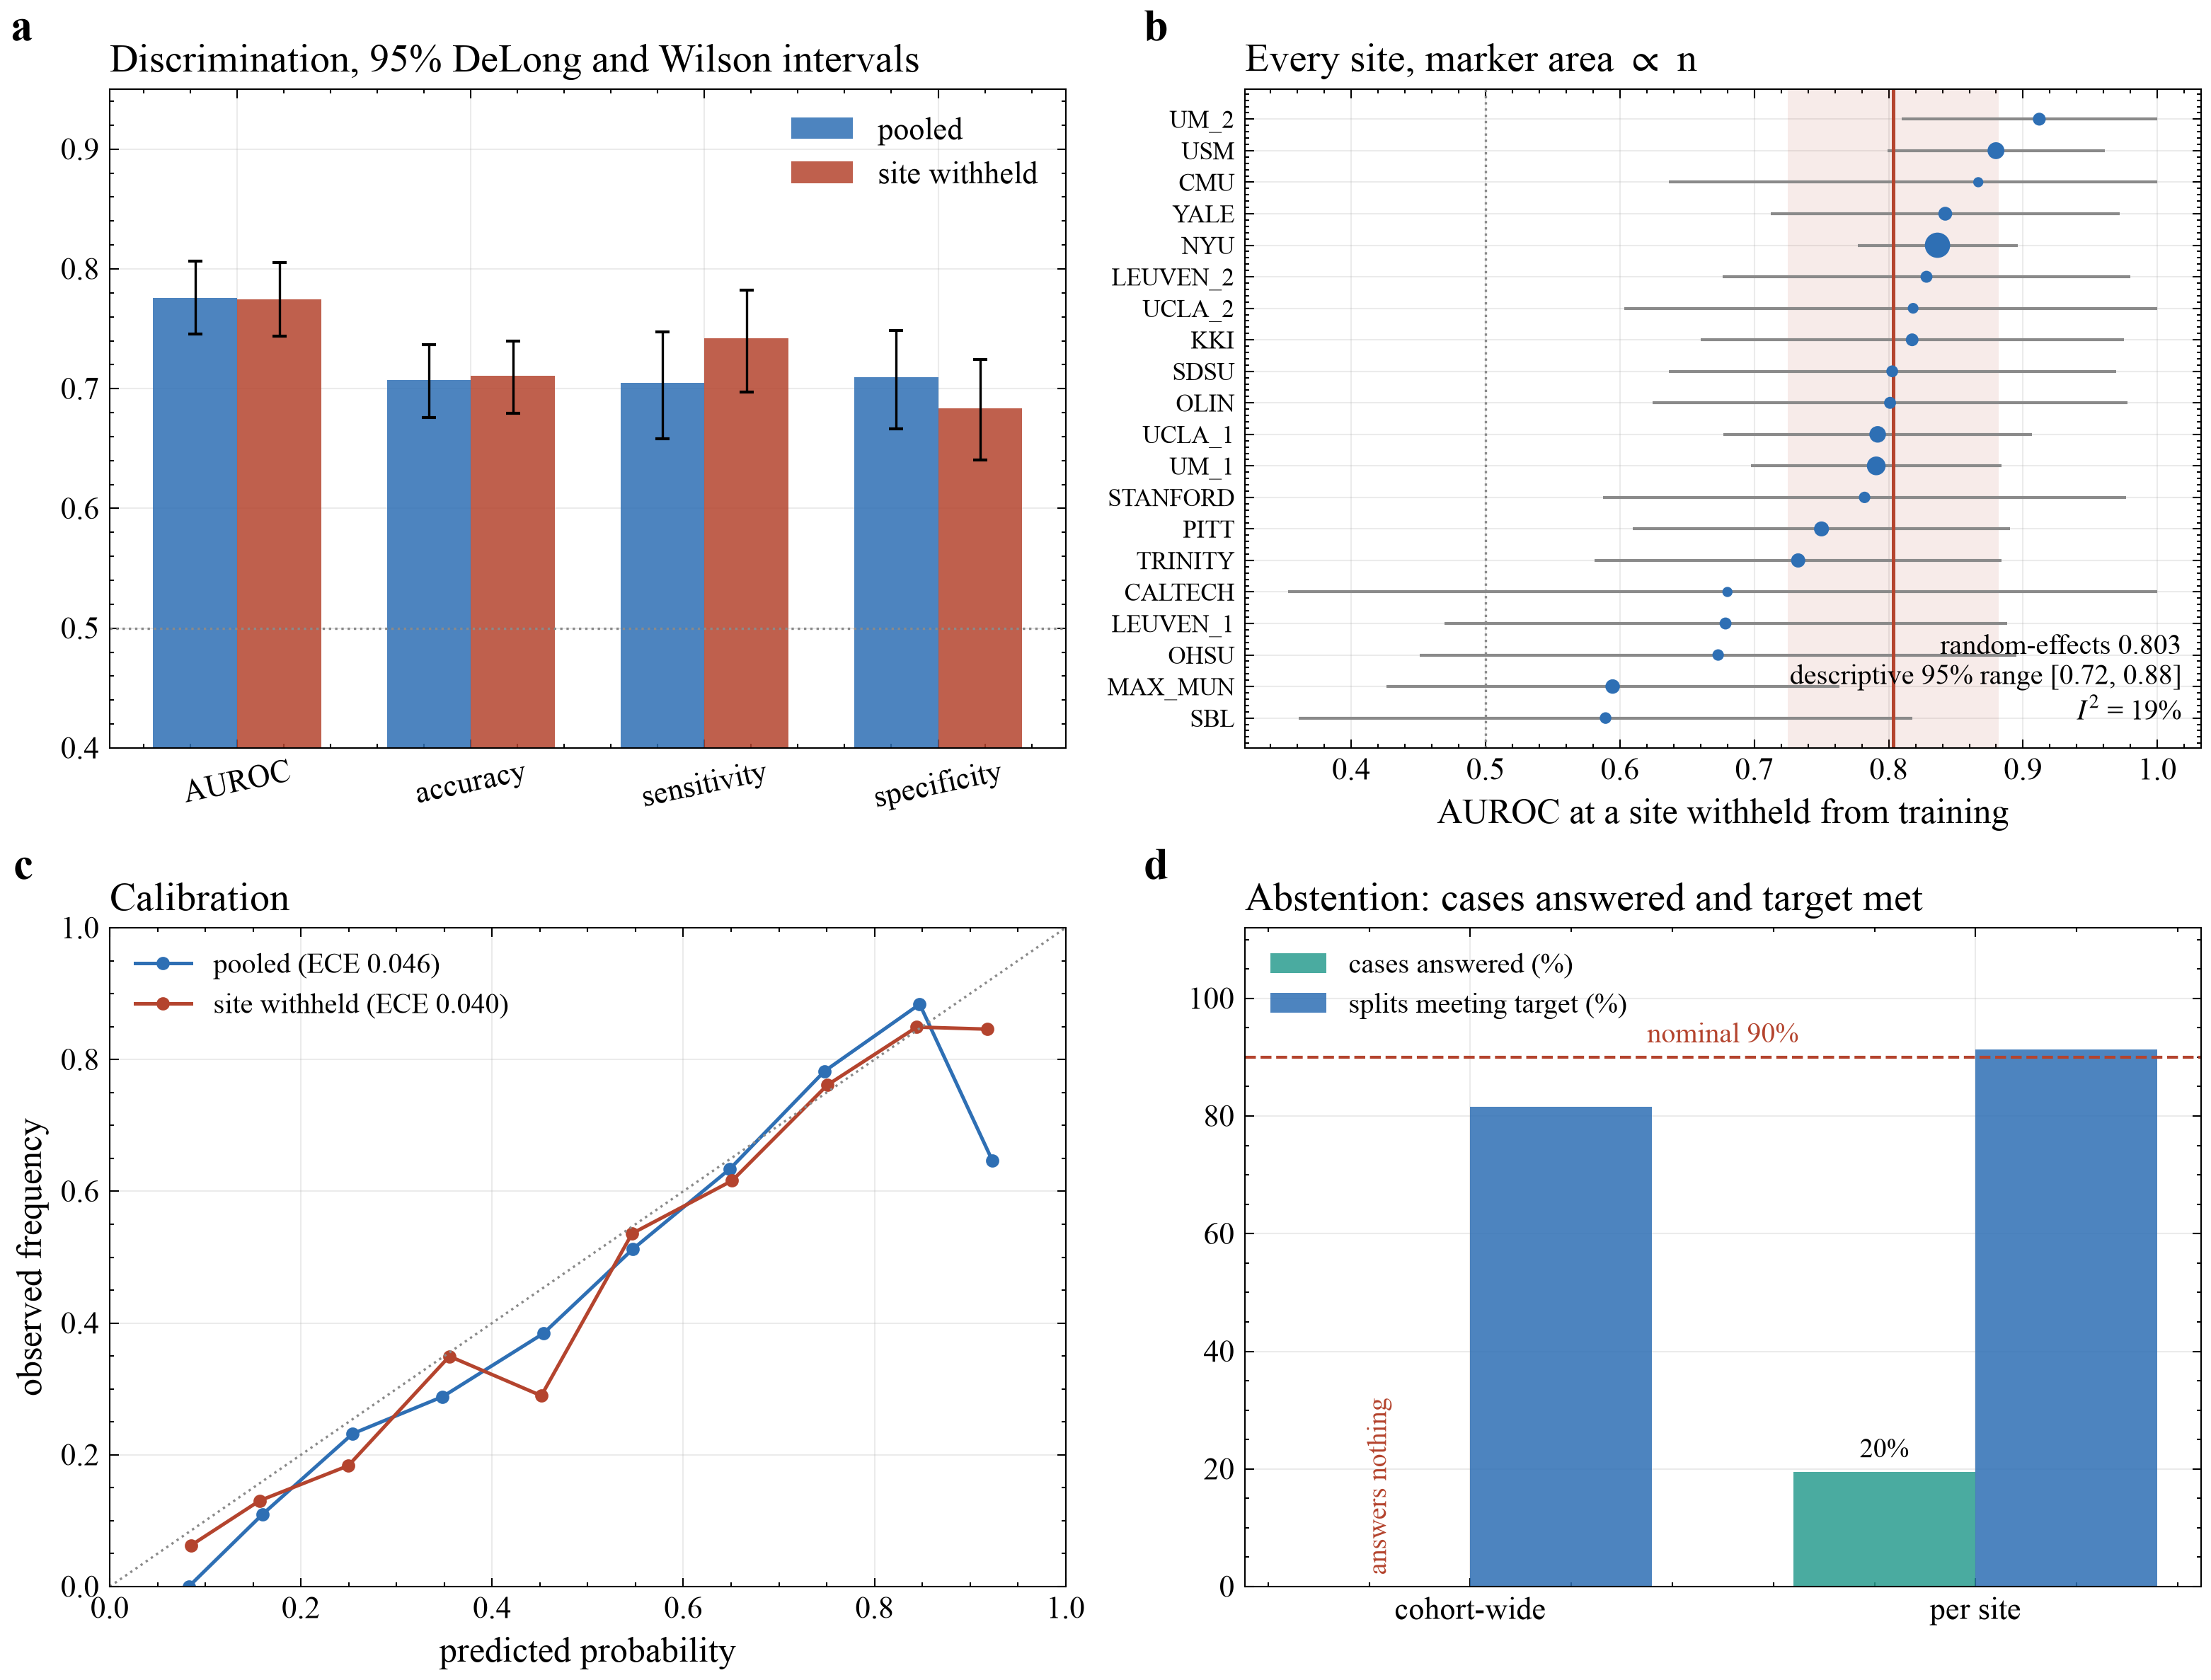
\includegraphics[width=\linewidth]{fig_performance}
\caption{Discrimination, per-site transfer, calibration, and abstention of the primary ensemble. (a) Discrimination under both validation protocols, with 95\% DeLong and Wilson intervals reported as lower-bound estimates of uncertainty. (b) AUROC for each site when that site is withheld from training, with marker area proportional to the number of participants. The random-effects mean and the descriptive interval from Equation~\eqref{eq:prediction-interval} are shown; this interval describes the observed sites and is not interpreted as a prediction for an unseen site. (c) Native predicted probabilities against observed frequencies in ten equal-width bins. (d) Cohort-wide and per-site abstention under LOSO validation, showing the percentage of participants answered when the threshold is set on the full sample and the percentage of held-out half-splits in which the error target is achieved, relative to the nominal 90\%.}
\label{fig:performance}
\end{figure}

Variation across sites is summarised with a random-effects model as a descriptive sensitivity analysis. Combining the 20 site-specific estimates gives a random-effects mean AUROC of 0.803 (Figure~\ref{fig:performance}b). Between-site heterogeneity is modest and not statistically distinguishable from chance ($Q=23.5$ on 19 degrees of freedom, $p=0.22$; $I^2=19\%$). The descriptive 95\% interval from Equation~\eqref{eq:prediction-interval} spans 0.725--0.882. Because LOSO estimates share training data, this interval is not treated as a validated prediction interval for an independent site. Site-level AUROC ranges from 0.589 at SBL to 0.912 at UM\_2. Two sites, SBL and MAX\_MUN, fall below 0.65, and the 95\% intervals of five sites (CALTECH, LEUVEN\_1, MAX\_MUN, OHSU, and SBL) include 0.5. These wide intervals are expected because the median site contains only about 30 participants. Phenotypic variables provide some additional discrimination but contribute little beyond connectivity. The phenotype model reaches an AUROC of about 0.62 on its own (Section~\ref{par:phenotype-model}), and adding it to the ensemble increases participant-pooled AUROC by about 0.004 (unadjusted $p=0.041$; $q=0.11$, reported for reference only). The phenotype member is therefore not retained. For comparison with published ABIDE-I studies, the wider QC cohort is used because its QC definition yields 1,035 eligible participants, matching the published count. Three participants lack usable time series, leaving 1,032 for analysis. In this cohort, pooled ten-fold validation gives a participant-pooled accuracy of 0.706 (95\% Wilson interval 0.678--0.733). Published accuracies of 0.700, 0.703, and 0.708 are reported by \citet{Heinsfeldetal2018}, \citet{Eslamietal2019}, and \citet{AlmuqhimSaeed2021}, respectively; these values are cited as reported and are not recomputed here.

\begin{table}[t]
\centering
\caption{Placement against published work on ABIDE-I resting-state functional
connectivity. Values for the other studies are as reported by their authors; n.r., not
reported. For the ensemble rows, AUROC is participant-pooled and accuracy is the fold mean,
which agrees with the participant-pooled value to three decimals. For the tangent-model
row, AUROC and accuracy are fold means. The unseen-site column gives the
LOSO AUROC, with its difference from the pooled ten-fold value in brackets.}
\label{tab:published-comparison}
\small
\setlength{\tabcolsep}{4pt}
\begin{tabular}{@{}>{\raggedright\arraybackslash}p{0.24\linewidth}cccccc@{}}
\toprule
Study & Accuracy & AUROC & Sample & Procedure & AUROC, unseen site & ECE \\
\midrule
\citet{Heinsfeldetal2018} & 0.700 & n.r. & 1,035 & 10-fold & n.r. & n.r. \\
\citet{Eslamietal2019} & 0.703 & n.r. & 1,035 & 10-fold & n.r. & n.r. \\
\citet{AlmuqhimSaeed2021} & 0.708 & n.r. & 1,035 & 10-fold & n.r. & n.r. \\
This work, ensemble & 0.707 & 0.776 & 871 & nested 10-fold & 0.774 ($-0.002$) & 0.046 \\
This work, ensemble, wider QC cohort & 0.706 & 0.789 & 1,032 & nested 10-fold & 0.783 ($-0.006$) & 0.023 \\
This work, tangent model, wider QC cohort & 0.696 & 0.766 & 1,032 & nested 10-fold & -- & -- \\
\bottomrule
\end{tabular}
\end{table}

The published accuracy values in Table~\ref{tab:published-comparison} are too close to support a clear separation between methods, particularly because the comparison studies do not report confidence intervals. With these sample sizes, the expected uncertainty is roughly $\pm0.03$, whereas the three published accuracies differ by only 0.008. Two additional measures are therefore reported for the present study without direct comparison to the published results. AUROC is 0.776 under pooled validation and 0.774 under LOSO validation, while the ECE is 0.046 (Section~\ref{subsec:results-calibration}). The present accuracy is also obtained without fitting outcome-dependent steps before the data split. This distinction is important because global label-informed feature selection produces a markedly higher performance estimate in Section~\ref{subsec:results-selection-scope}. Performance also varies with cohort definition. The static tangent model reaches a fold-mean AUROC of 0.756 in the primary cohort of 871 participants and 0.766 in the wider cohort of 1,032 participants. Because many participants excluded by the primary definition have greater head motion or preprocessing problems, and these exclusions are not balanced across diagnostic groups, the difference between cohorts may partly reflect data quality and cohort composition rather than connectivity alone.

\subsection{Cognitive ability and detection}
\label{subsec:results-cognitive-ability}

Discrimination is lower in the higher-IQ autistic subgroups in the unmatched band analysis, contributing to the fourth study contribution. Because these subgroup analyses are exploratory (Sections~\ref{par:cognitive-sex-subgroups} and~\ref{subsubsec:analysis-status}), the pattern is interpreted descriptively. To keep the comparison group constant, all 468 non-autistic participants are used as the reference for every IQ band, while only autistic participants are divided by full-scale IQ. Under pooled ten-fold validation, AUROC decreases from 0.873 for autistic participants with full-scale IQ below 85 to 0.719 for those with IQ 115 or above (Table~\ref{tab:iq-bands}; Figure~\ref{fig:group-differences}d). A similar pattern is observed under LOSO validation, where AUROC decreases from 0.871 to 0.709. However, the autistic IQ bands still differ from the fixed non-autistic reference group in full-scale IQ, so this unmatched comparison does not isolate IQ from group composition. The matched analysis below addresses this remaining difference.

\begin{table}[t]
\centering
\caption{AUROC by full-scale IQ band of the autistic participants, each band scored
against the same comparison group of all 468 non-autistic participants.}
\label{tab:iq-bands}
\small
\begin{tabular}{@{}lccc@{}}
\toprule
Autistic participants & $n$ & Pooled ten-fold & LOSO \\
\midrule
Full-scale IQ below 85 & 40 & 0.873 & 0.871 \\
Full-scale IQ 85--99 & 97 & 0.815 & 0.816 \\
Full-scale IQ 100--114 & 126 & 0.781 & 0.788 \\
Full-scale IQ 115 or above & 113 & 0.719 & 0.709 \\
\bottomrule
\end{tabular}
\end{table}

\begin{figure}[pos=tbp]
\centering
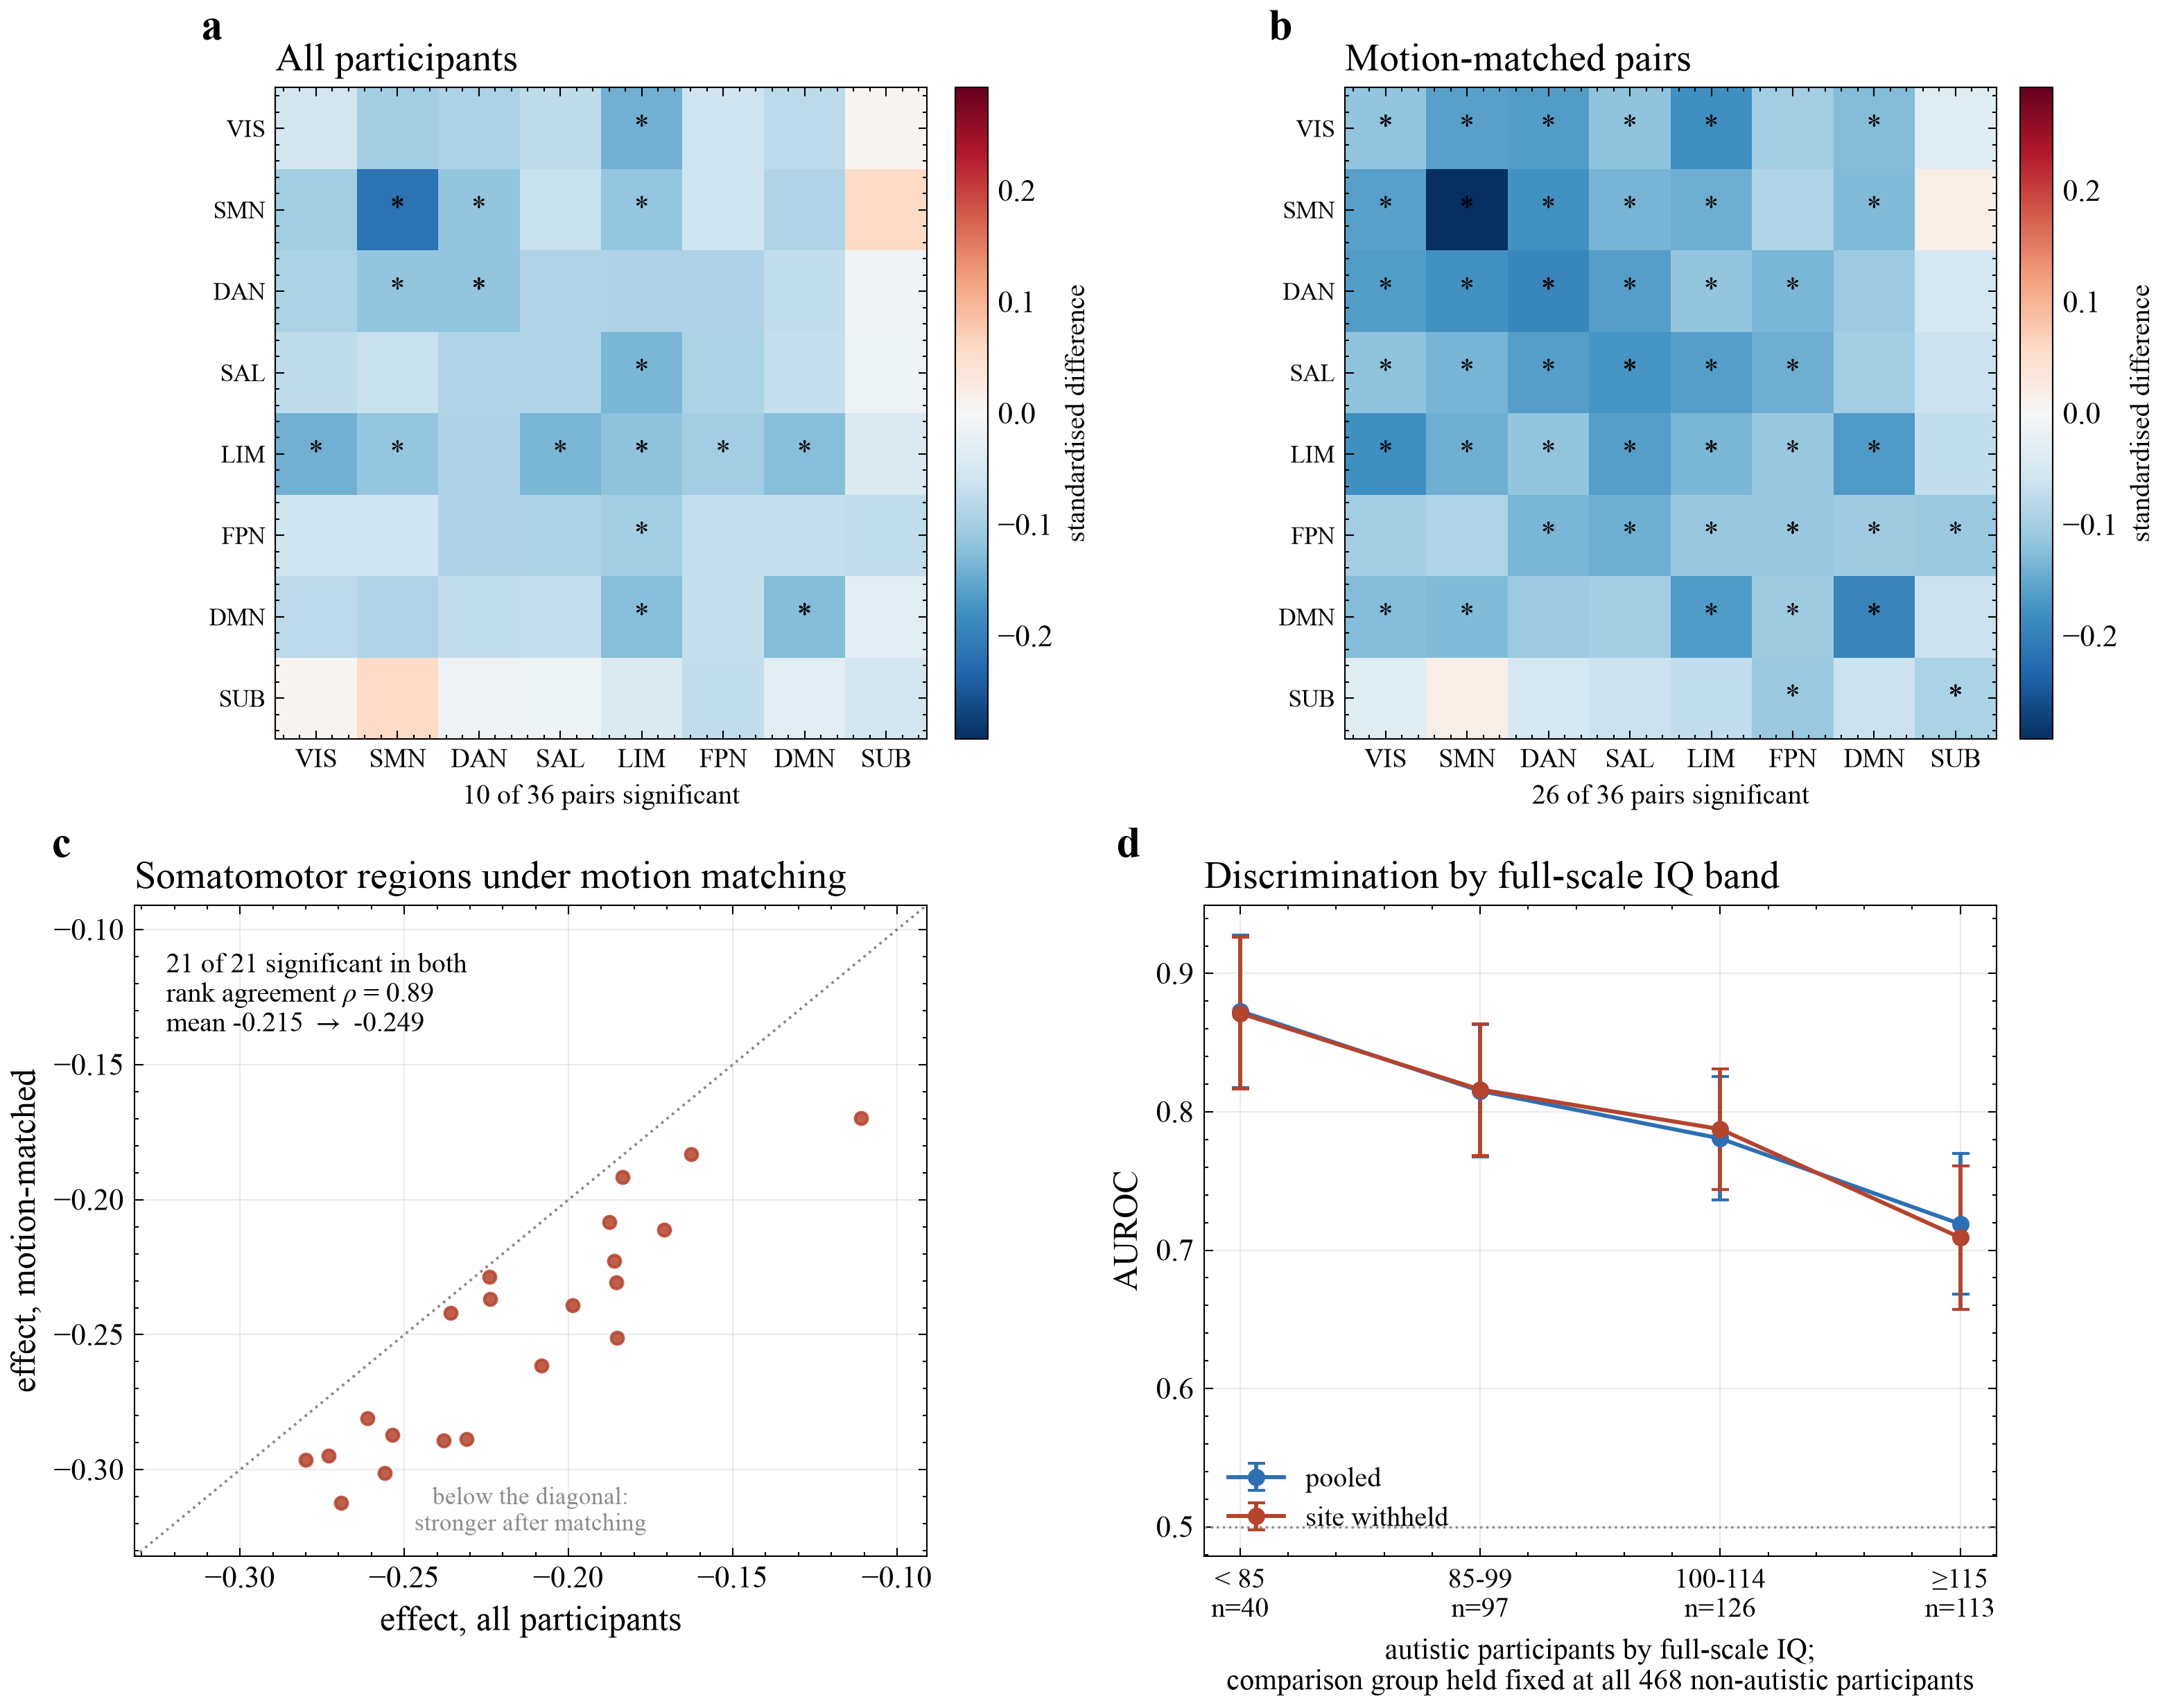
\includegraphics[width=\linewidth]{fig_groupdiff}
\caption{Group differences in functional-system connectivity and the effect of motion
matching. (a, b) Standardised difference for every pair of systems (system codes as in Figure~\ref{fig:overview}) in all participants and
in within-site pairs matched for head motion, on a shared colour scale; asterisks mark
pairs with BH-FDR $q<0.05$. (c) The effect of each somatomotor region in all
participants plotted against its effect in motion-matched pairs; points below the diagonal
are stronger once motion is matched. (d) Discrimination by full-scale IQ band among
autistic participants (below 85, 85--99, 100--114, and 115 or above), each against all 468
non-autistic participants, under both validation protocols.}
\label{fig:group-differences}
\end{figure}

The same pattern is observed when both groups are divided into quartiles of site-centred full-scale IQ (Table~\ref{tab:iq-quartiles}). Under pooled ten-fold validation, AUROC decreases from 0.833 in the lowest quartile to 0.709 in the highest. Because autistic participants have lower full-scale IQ overall (Table~\ref{tab:participants}), this stratified comparison may still reflect differences in IQ between the groups. To reduce this imbalance, autistic participants are matched to non-autistic participants from the same site within five full-scale IQ points. This produces 274 matched pairs under pooled ten-fold validation and 275 pairs under LOSO validation.

\begin{table}[t]
\centering
\caption{AUROC by quartile of site-centred full-scale IQ, in all participants and in
participants matched on full-scale IQ within site. The matched counts are given for pooled
ten-fold and LOSO validation, respectively.}
\label{tab:iq-quartiles}
\small
\begin{tabular}{@{}lcccccc@{}}
\toprule
 & \multicolumn{3}{c}{All participants} & \multicolumn{3}{c}{IQ-matched participants} \\
\cmidrule(lr){2-4}\cmidrule(l){5-7}
Quartile & $n$ & Pooled ten-fold & LOSO & $n$ (pooled / LOSO) & Pooled ten-fold & LOSO \\
\midrule
Q1 & 204 & 0.833 & 0.825 & 137 / 144 & 0.855 & 0.848 \\
Q2 & 203 & 0.794 & 0.793 & 137 / 132 & 0.700 & 0.735 \\
Q3 & 201 & 0.746 & 0.745 & 138 / 137 & 0.751 & 0.737 \\
Q4 & 203 & 0.709 & 0.705 & 136 / 137 & 0.756 & 0.756 \\
\bottomrule
\end{tabular}
\end{table}

After IQ matching, discrimination remains highest in the lowest quartile but no longer declines consistently across the upper three. Under pooled ten-fold validation, AUROC is 0.855 in the lowest quartile and ranges from 0.700 to 0.756 in the remaining quartiles; under LOSO validation, the corresponding values are 0.848 and 0.735--0.756. This suggests that part of the original IQ gradient reflects between-group differences in IQ. Complementary within-group analyses show a negative association between classifier score and cognitive ability among autistic participants, but not among non-autistic participants. After adjustment for site, age, and mean FD, the pooled ten-fold score correlates with full-scale IQ at $\rho=-0.180$ ($p=0.0004$, $n=376$) in autistic participants, compared with $\rho=+0.048$ ($p=0.3208$, $n=435$) in non-autistic participants. Similar patterns are observed for verbal and performance IQ and under both validation protocols. Diagnosis-by-IQ interaction models further test this difference directly while adjusting for age, sex, mean FD, and site. The interaction remains significant after BH-FDR correction for full-scale IQ ($\beta=-0.176$, $q=0.025$) and verbal IQ ($\beta=-0.205$, $q=0.025$) under pooled ten-fold validation, and for both measures under LOSO validation ($q=0.033$). The interaction for performance IQ does not survive correction ($q=0.082$). These results indicate that the negative association between classifier score and cognitive ability is stronger in autistic participants for full-scale and verbal IQ.

\begin{table}[t]
\centering
\caption{Spearman correlation between classifier score and IQ within each diagnostic group, reported as $\rho$ ($p$). Before correlation, both variables are residualised for site, age, and mean FD. The p-values are not adjusted for multiple comparisons.}
\label{tab:iq-correlations}
\small
\setlength{\tabcolsep}{4pt}
\begin{tabular}{@{}lccccc@{}}
\toprule
 & & \multicolumn{2}{c}{Autistic} & \multicolumn{2}{c}{Non-autistic} \\
\cmidrule(lr){3-4}\cmidrule(l){5-6}
Measure & $n$ (autistic / non-autistic) & Pooled ten-fold & LOSO & Pooled ten-fold & LOSO \\
\midrule
Full-scale IQ & 376 / 435 & $-0.180$ (0.0004) & $-0.179$ (0.0005) & $+0.048$ (0.3208) & $+0.022$ (0.6466) \\
Verbal IQ & 342 / 379 & $-0.182$ (0.0007) & $-0.189$ (0.0004) & $+0.039$ (0.4547) & $+0.001$ (0.9892) \\
Performance IQ & 344 / 391 & $-0.152$ (0.0047) & $-0.147$ (0.0062) & $+0.007$ (0.8862) & $-0.005$ (0.9271) \\
\bottomrule
\end{tabular}
\end{table}

The absence of a comparable score--IQ association in non-autistic participants argues against a general relation between cognitive ability and classifier score. This interpretation is strengthened by the diagnosis-by-IQ interaction results, which remain significant for full-scale and verbal IQ, although full-scale IQ varies less among non-autistic participants (Table~\ref{tab:participants}). The association is also consistent with the verbal-IQ dependence reported in ABIDE by \citet{Nielsenetal2013}. However, the IQ-matched upper quartiles do not show a monotonic decline in AUROC, so the exploratory analyses do not establish a simple IQ-specific gradient in detectability. Instead, they indicate that measured ABIDE-I performance varies with the cognitive composition of the autistic sample, such that the same method can yield different AUROC values in cohorts with different IQ distributions. No corresponding reduction in discrimination is observed among female participants. Under pooled ten-fold validation, AUROC is 0.827 (0.760--0.895, $n=144$) in female participants and 0.764 (0.730--0.798, $n=727$) in male participants; under LOSO validation, the corresponding values are 0.806 (0.735--0.878) and 0.767 (0.733--0.801). Because these intervals overlap and the female subgroup is small, no sex difference in discrimination is inferred.

\subsection{Functional-system differences under motion matching}
\label{subsec:results-system-differences}

Functional-system differences are examined as exploratory group contrasts, and the motion-matched somatomotor result contributes to the third study contribution. To reduce the 19,110 connection-level effects to a more interpretable scale, regions are grouped into the seven cortical systems of \citet{Yeoetal2011} plus a subcortical/cerebellar class, producing 36 system pairs with 21--1,462 connections each (median 441). Connection values are adjusted for acquisition site, mean framewise displacement, age, and sex before system-level effects are calculated, and significance is assessed by permuting diagnostic labels within site. In the 863-participant group-contrast cohort, 10 of 36 system pairs remain significant after correction, and all show lower connectivity in autistic participants (Table~\ref{tab:system-pairs}; Figure~\ref{fig:group-differences}a). Overall, 34 of 36 system-pair effects are negative, with no significant increases. The largest reduction occurs within the somatomotor system (standardised difference $-0.215$, $z=-4.769$, $q=0.002$), while the limbic system shows differences across the widest range of system pairs. Because both nuisance adjustment and permutation account for site, these effects reflect group differences after controlling for site-related variation in connectivity.

\begin{table}[t]
\centering
\caption{Functional-system pairs with the largest standardised group differences in the group-contrast cohort of 863 participants. Negative values indicate lower connectivity in autistic participants, and $q$ denotes the BH-FDR-adjusted permutation p-value. The first ten rows correspond to pairs with $q<0.05$.}
\label{tab:system-pairs}
\small
\begin{tabular}{@{}llcccc@{}}
\toprule
System & System & Connections & Difference & $z$ & $q$ \\
\midrule
Somatomotor & Somatomotor & 210 & $-0.215$ & $-4.769$ & 0.002 \\
Limbic & Visual & 210 & $-0.140$ & $-3.633$ & 0.002 \\
Limbic & Salience / ventral attention & 147 & $-0.133$ & $-3.247$ & 0.013 \\
Default mode & Default mode & 903 & $-0.127$ & $-3.777$ & 0.002 \\
Default mode & Limbic & 301 & $-0.125$ & $-3.677$ & 0.004 \\
Limbic & Limbic & 21 & $-0.118$ & $-3.052$ & 0.014 \\
Dorsal attention & Somatomotor & 399 & $-0.116$ & $-2.653$ & 0.024 \\
Dorsal attention & Dorsal attention & 171 & $-0.115$ & $-2.875$ & 0.024 \\
Limbic & Somatomotor & 147 & $-0.114$ & $-2.839$ & 0.024 \\
Frontoparietal control & Limbic & 147 & $-0.102$ & $-2.733$ & 0.024 \\
Somatomotor & Visual & 630 & $-0.101$ & $-2.317$ & 0.058 \\
Frontoparietal control & Salience / ventral attention & 441 & $-0.093$ & $-2.317$ & 0.058 \\
\bottomrule
\end{tabular}
\end{table}

Because permutation testing operates on residualised connections, a separate motion-matched analysis is used to examine whether the group differences persist when autistic and non-autistic participants are closely matched on mean FD within site (Section~\ref{subsubsec:system-motion-regional}). Under the system-level caliper, 256 pairs are retained and the group difference in motion is removed ($p=7.6\times10^{-7}$ before matching and $p=0.59$ after). In this matched sample, 26 of 36 system pairs are significant, compared with 10 of 36 in the full cohort, although the change in count cannot be attributed to motion matching alone because the matched sample also differs in size and composition. The somatomotor within-system effect strengthens from $-0.2155$ ($z=-4.77$) to $-0.2925$ ($z=-4.89$). At the regional level, all 21 somatomotor regions are significant in the full cohort, with the strongest effects in the postcentral gyrus, paracentral lobule, and precentral gyrus. Using the wider regional caliper, 280 matched pairs are retained and the motion difference is again removed ($p=0.28$). All 21 regions remain significant, every regional effect strengthens, and the ordering is preserved (rank correlation 0.89), while the mean regional effect changes from $-0.215$ to $-0.249$ (Figure~\ref{fig:group-differences}c). Freedman--Lane residual permutation gives the same overall pattern: reduced connectivity is found in 14 of 36 system pairs before matching and 27 of 36 after matching, all in the negative direction, while the somatomotor effect strengthens from $-0.226$ to $-0.294$. These values are regression-scale effects and are therefore not directly comparable with the standardised regional effects above. The regional ranking shows moderate internal stability, with a split-half correlation of 0.55 across the 21 regions, compared with 0.38 for all 210 within-system connections and 0.34 for the top 50. Random blocks of 21 regions have a median stability of 0.35, and 9\% reach the somatomotor value. Mean FD is also positively associated with mean connection strength ($\rho=+0.51$ across participants and $+0.45$ within site), so the observed reduction is opposite to the direction expected from residual motion alone. The somatomotor finding is consistent with earlier reports \citep{Chenetal2015,Holigaetal2019,Ilioskaetal2023}, although overlap in ABIDE participants prevents treating this agreement as independent replication. Overall, the somatomotor reduction persists and strengthens after matching on recorded mean FD, but residual motion cannot be fully excluded, the contrasts do not show which features the classifier uses, and the results remain conditional on the chosen preprocessing strategy without global signal regression.

\subsection{Feature-selection scope and granularity}
\label{subsec:results-selection-scope}

The effect of data-access scope on measured performance is examined across seven conditions using identical folds and the 19,900 static tangent features of the primary cohort (Section~\ref{par:selection-scope}; Table~\ref{tab:selection-scope}). These analyses are reported as methodological checks rather than as study contributions. Fitting the tangent reference globally, or fitting both the reference and scaler globally, changes fold-mean AUROC by no more than 0.003. Similarly, selecting the regularisation constant on the held-out fold gives an AUROC of 0.758, while adding acquisition site as a predictor gives 0.756. These results show that these changes in data-access scope have little effect on performance compared with the much larger effect of label-informed feature selection examined next.

\begin{table}[t]
\centering
\caption{Fold-mean AUROC across seven data-access conditions, evaluated using 19,900 static tangent features in the primary cohort of 871 participants with identical outer folds. SD is calculated across the outer folds.}
\label{tab:selection-scope}
\small
\begin{tabular}{@{}>{\raggedright\arraybackslash}p{0.62\linewidth}cc@{}}
\toprule
Condition & AUROC & SD \\
\midrule
Reference: every step fitted within the training partition & 0.756 & 0.048 \\
Tangent reference fitted on all participants & 0.756 & 0.048 \\
Tangent reference and scaler fitted on all participants & 0.753 & 0.049 \\
Regularisation constant chosen on the held-out fold & 0.758 & 0.048 \\
Acquisition site added as a predictor & 0.756 & 0.049 \\
Tangent reference fitted on all participants and 2,000 of 19,900 connections selected with all diagnostic labels & 0.987 & 0.008 \\
All five changes combined & 0.988 & 0.008 \\
\bottomrule
\end{tabular}
\end{table}

In contrast, selecting 2,000 of 19,900 connections with an F test using all diagnostic labels before CV raises fold-mean AUROC from 0.756 to 0.987 and accuracy from 0.692 to 0.948 on the same folds. Because fitting the tangent reference globally leaves AUROC unchanged at 0.756, the increase is driven primarily by the label-informed selection step. Applying all data-access changes together gives an AUROC of 0.988, showing little additional effect beyond selection. Thus, among the tested conditions, only global connection-level feature selection changes AUROC by more than 0.003, whereas held-out tuning and the other scope changes have minimal effects. Estimates from pipelines that select connections before CV are therefore not directly comparable with estimates from nested selection. Region-level selection shows a different pattern (Table~\ref{tab:region-selection}; Figure~\ref{fig:corrections}c). Ranking regions with all labels or with training-fold labels changes AUROC by only 0.006 on average across models retaining 10--100 of 196 regions, with differences ranging from 0.001 at 10 regions to 0.012 at 100 and no consistent direction. Refitting the nuisance model within each outer-training partition changes the training-fold condition by only 0.0035 on average and at most 0.0085, while preserving the ordering across list lengths; all restricted models remain below the model using all 196 regions (0.781). These findings are consistent with greater sensitivity of fine-grained connection selection to label access than region-level selection. However, the two analyses also differ in cohort size, shrinkage, ranking statistic, and AUROC summary, so feature granularity cannot be isolated as the only explanation.

\begin{table}[t]
\centering
\caption{Participant-pooled AUROC when the top-ranked regions are chosen with all
diagnostic labels or with the labels of each training fold only, in the group-contrast
cohort (863 participants and 196 regions). All 196 regions give 0.781.}
\label{tab:region-selection}
\small
\begin{tabular}{@{}ccc@{}}
\toprule
Regions kept & Chosen with all labels & Chosen within each fold \\
\midrule
10 & 0.628 & 0.627 \\
20 & 0.660 & 0.656 \\
30 & 0.699 & 0.702 \\
50 & 0.738 & 0.748 \\
100 & 0.764 & 0.752 \\
\bottomrule
\end{tabular}
\end{table}

\begin{figure}[pos=tbp]
\centering
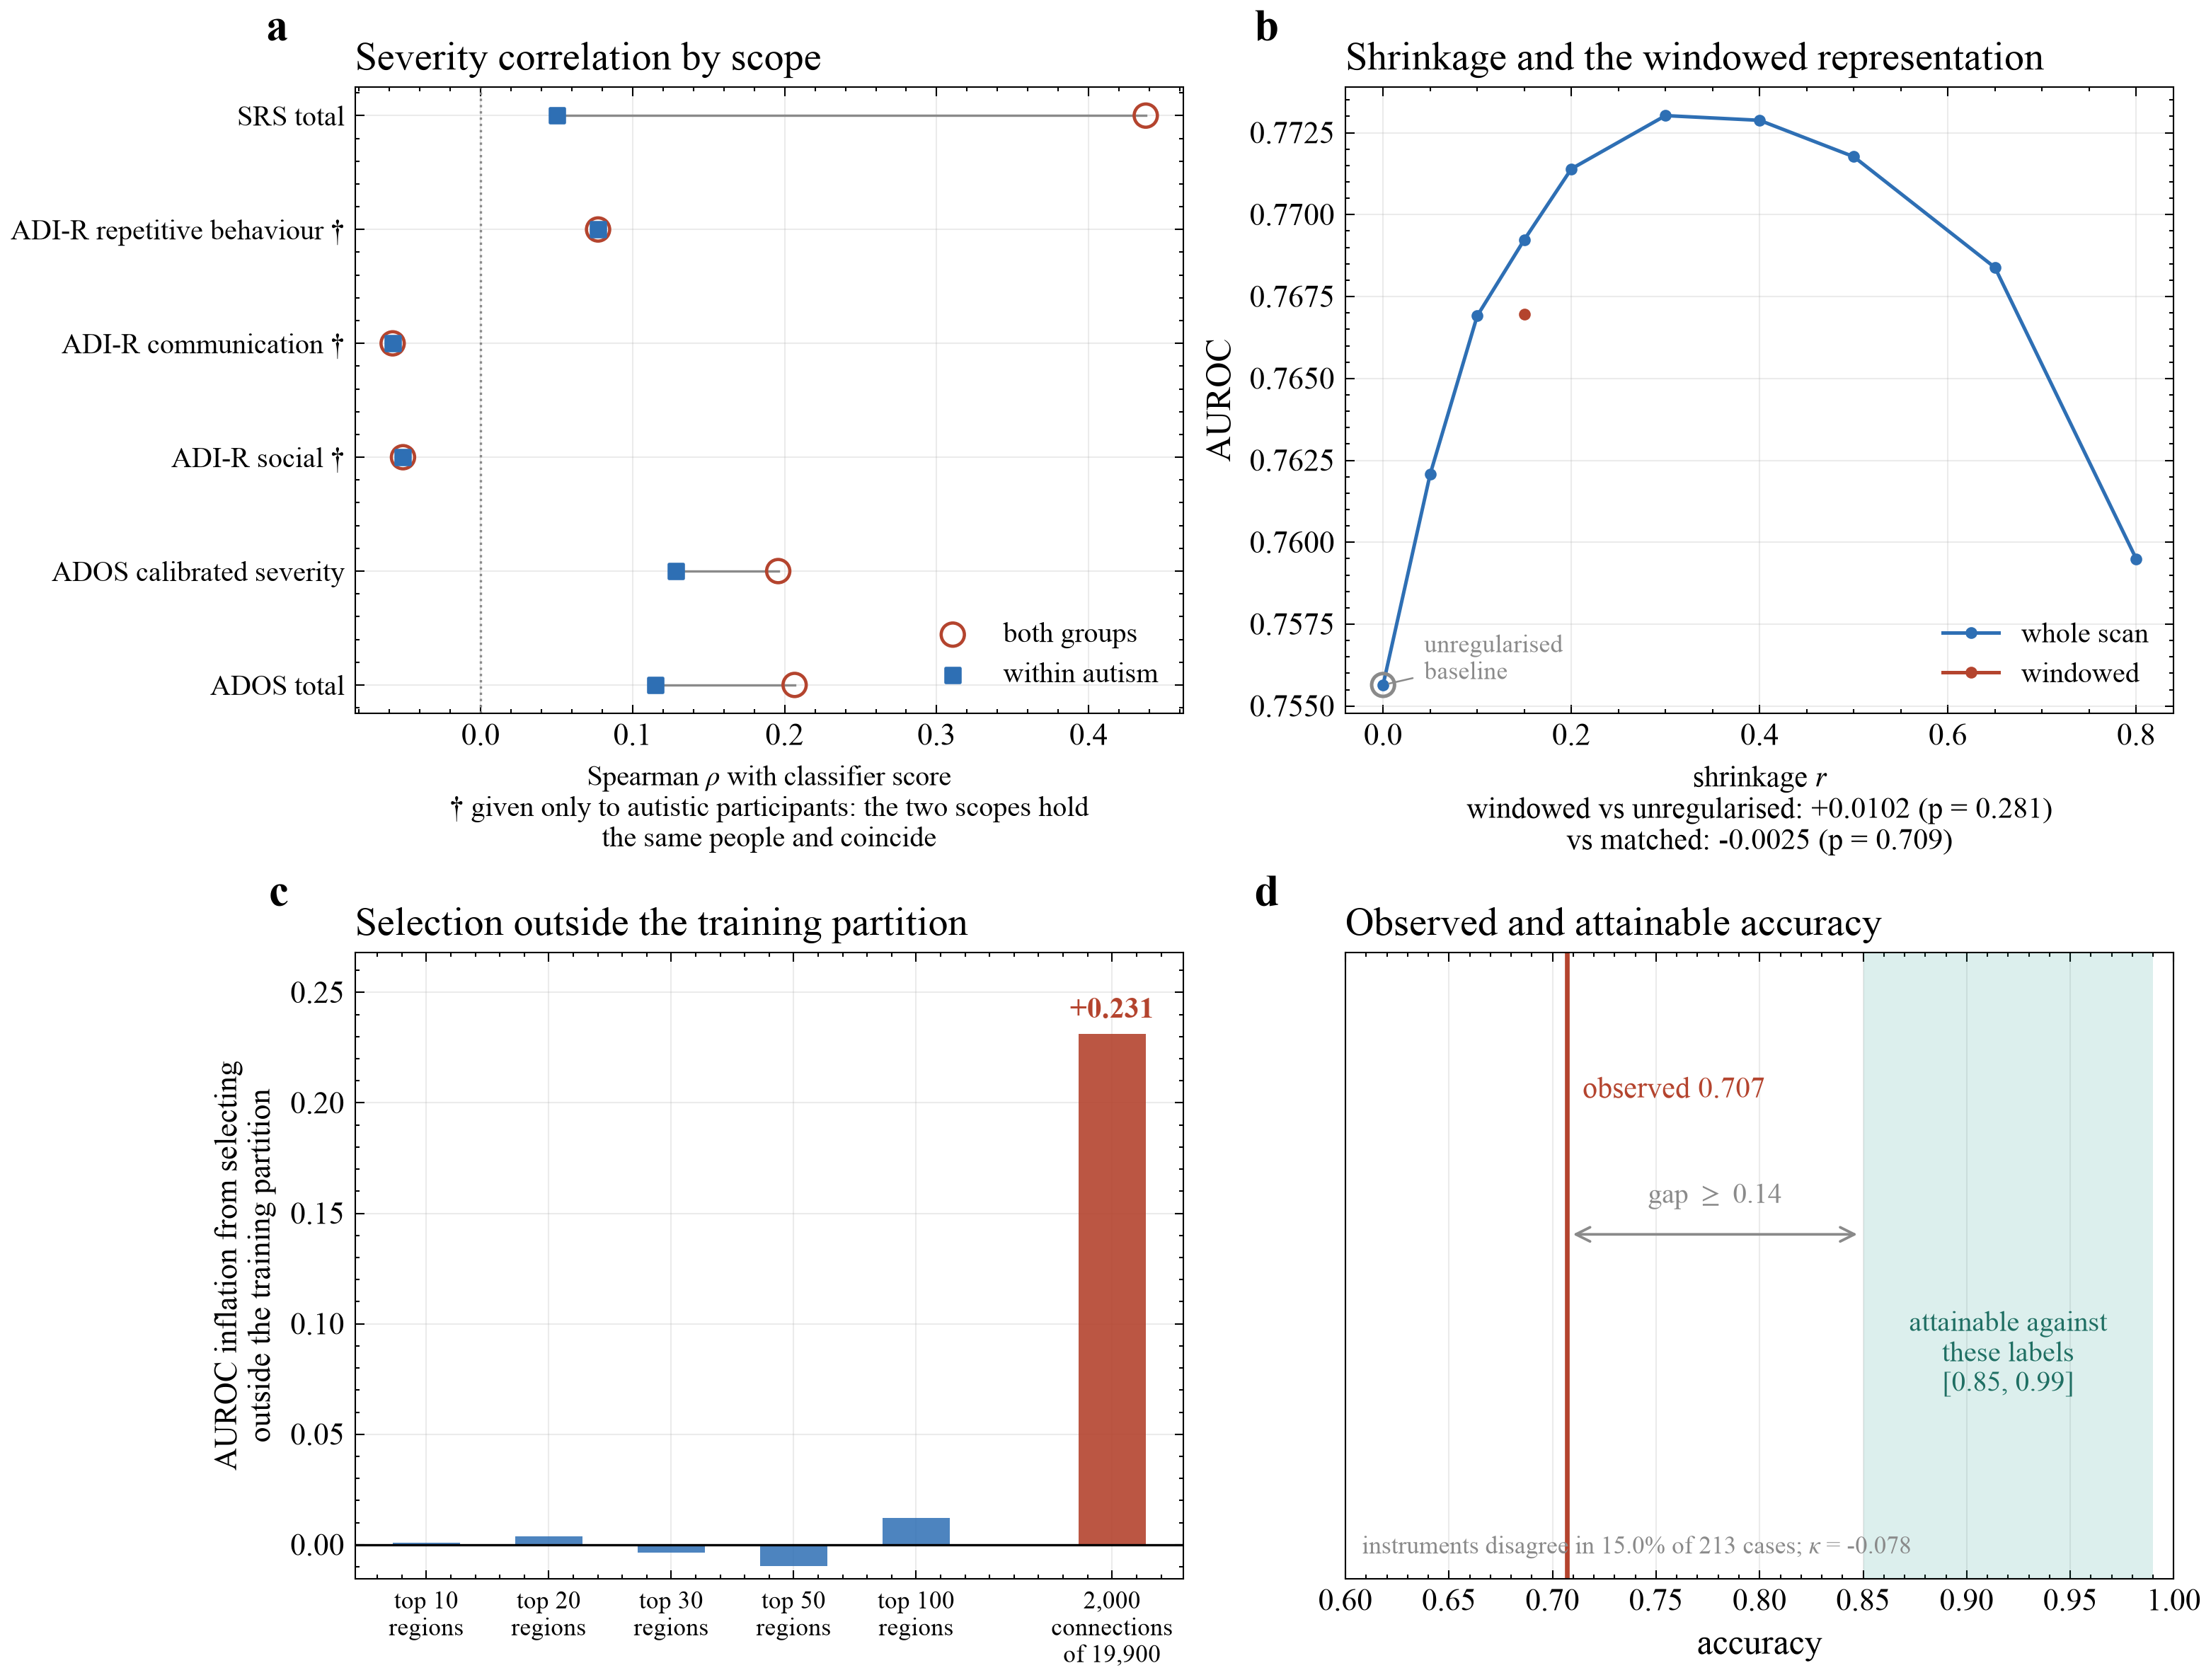
\includegraphics[width=\linewidth]{fig_corrections}
\caption{Four effects that change when the corresponding control is applied. (a)
Correlation between classifier score and symptom severity under pooled ten-fold validation,
computed across both groups and within the autistic group; rows marked with a dagger are
instruments given only to autistic participants, for which the two scopes necessarily coincide.
(b) AUROC of whole-scan connectivity across shrinkage levels, with the windowed
representation placed at the shrinkage that it applies to its own windows. (c) AUROC
inflation from selection outside the training partition, for 10 to 100 of 196 regions and
for 2,000 of 19,900 connections. (d) Observed accuracy against the interval of accuracy
attainable given the diagnostic labels.}
\label{fig:corrections}
\end{figure}

Restricting the model to the most discriminating regions reduces performance at every list length. Using all 196 regions gives an AUROC of 0.781, higher than any reduced set in Table~\ref{tab:region-selection}, while the smallest subset is lower by 0.154. This pattern suggests that discriminative information is distributed across many regions rather than concentrated only in those with the largest group differences. Region restriction therefore provides no performance advantage in these data. More broadly, the published accuracy range is already reached without feature selection before the split. In the wider cohort, the ensemble achieves a participant-pooled accuracy of 0.706 under pooled ten-fold validation (Section~\ref{subsec:results-performance}), compared with published values of 0.700, 0.703, and 0.708 for the same eligible count of 1,035 participants. Accuracy at this level therefore does not require selection outside the training partition.

\subsection{Classifier family}
\label{subsec:results-classifier-family}

Linear classifiers perform better than the evaluated fixed-configuration tree ensembles on static tangent connectivity, forming part of the fifth study contribution. All eight classifiers use the same features, scaling procedure, and outer folds (Section~\ref{par:classifier-family}), so the comparison is made under a common input and validation setting. The five linear classifiers achieve participant-pooled AUROCs of 0.735--0.757, compared with 0.611--0.624 for random forest, XGBoost, and CatBoost (Table~\ref{tab:classifier-family}). Penalised logistic regression gives the highest AUROC at 0.757, followed closely by ridge classification at 0.755 and linear SVC at 0.753. Shrinkage LDA and the rank-20 spectral model achieve AUROCs of 0.741 and 0.735, respectively. Because only logistic regression is tuned, these results compare the specified classifier configurations rather than the best attainable performance of each model family.

\begin{table}[t]
\centering
\caption{Classifier family on the static tangent features of the primary cohort
(871 participants), with identical features, scaling and outer folds. Only logistic
regression is tuned; the other classifiers use fixed configurations.}
\label{tab:classifier-family}
\small
\setlength{\tabcolsep}{4pt}
\begin{tabular}{@{}lcccc@{}}
\toprule
Classifier & AUROC (participant-pooled) & AUROC (fold mean) & SD (folds) & Accuracy (fold mean) \\
\midrule
Logistic regression & 0.757 & 0.756 & 0.048 & 0.692 \\
Ridge & 0.755 & 0.755 & 0.047 & 0.693 \\
Linear SVC & 0.753 & 0.753 & 0.048 & 0.687 \\
Shrinkage LDA (PCA-200) & 0.741 & 0.739 & 0.052 & 0.669 \\
Low-rank spectral (rank 20) & 0.735 & 0.737 & 0.044 & 0.672 \\
CatBoost & 0.624 & 0.623 & 0.042 & 0.597 \\
XGBoost & 0.617 & 0.616 & 0.050 & 0.584 \\
Random forest & 0.611 & 0.609 & 0.049 & 0.577 \\
\bottomrule
\end{tabular}
\end{table}

The performance gap between logistic regression and the tree ensembles is substantial. Logistic regression exceeds XGBoost by 0.1396 AUROC, random forest by 0.1461, and CatBoost by 0.1327, with unadjusted DeLong $p$-values ranging from $6.3\times10^{-15}$ to $2.4\times10^{-12}$ (Section~\ref{subsubsec:paired-comparisons}). By comparison, the rank-20 spectral model is 0.0214 below logistic regression (unadjusted $p=0.0439$; $q=0.1065$, reported for reference only). These results describe the specific configurations evaluated rather than the best possible performance of each classifier family, because only logistic regression is tuned while the tree ensembles use fixed settings (Section~\ref{par:classifier-family}). However, the fixed-configuration ridge, linear SVC, and LDA models also outperform all three tree ensembles. The stronger performance of the linear configurations therefore cannot be explained by logistic-regression tuning alone.

\subsection{Scope of the symptom-severity associations}
\label{subsec:results-symptom-severity}

The symptom analyses show that classifier scores are associated with symptom measures mainly when both diagnostic groups are analysed together, forming part of the fourth study contribution (Figure~\ref{fig:corrections}a). Under pooled ten-fold validation, 3 of 6 associations survive BH-FDR correction across both groups, whereas none survives within autistic participants alone (Section~\ref{par:symptom-associations}). The clearest example is the SRS total, for which the correlation falls from $\rho=0.438$ across both groups ($n=300$) to 0.050 within autistic participants ($n=163$). The corresponding values are 0.207 versus 0.115 for ADOS total and 0.196 versus 0.128 for ADOS calibrated severity. For the ADI-R domains, the correlations are unchanged because these measures are available only for autistic participants. These results indicate that the pooled associations largely reflect diagnostic-group separation, while an association between classifier score and symptom severity within autistic participants is not established.

\subsection{Windowed connectivity and covariance shrinkage}
\label{subsec:results-windowed-shrinkage}

The apparent advantage of windowed connectivity is small and disappears when the whole-scan representation receives the same additional covariance shrinkage, forming part of the fifth study contribution (Figure~\ref{fig:corrections}b). The windowed representation applies an additional shrinkage of 0.15 to its covariance estimates, whereas the original static representation does not (Section~\ref{subsubsec:primary-comparisons}). Applying the same shrinkage to the static representation increases its AUROC by 0.013 (unadjusted DeLong $p=0.004$). By comparison, the windowed representation exceeds the unshrunk static baseline by 0.010 ($p=0.281$) but differs from the shrinkage-matched static baseline by only $-0.002$ ($p=0.709$). Thus, the observed windowed advantage is consistent with the effect of additional covariance shrinkage rather than with added information from windowing itself.

\subsection{Calibration and recalibration within the training partitions}
\label{subsec:results-calibration}

The native ensemble probabilities show calibration slopes close to one but a small systematic offset in their average predicted risk, and training-partition recalibration removes this offset without changing discrimination; this forms the first study contribution (Table~\ref{tab:calibration-recalibration}; Figure~\ref{fig:calibration}). Under pooled ten-fold validation, the native calibration slope is 1.117 (95\% site-clustered bootstrap interval 0.901--1.325), and under LOSO validation it is 1.120 (0.866--1.366), with both intervals including one. Calibration-in-the-large is $-0.162$ ($-0.287$ to $-0.048$) under pooled validation and $-0.181$ ($-0.389$ to 0.019) under LOSO validation, indicating that the native probabilities tend to overestimate autism prevalence on average. The Brier score is 0.194 under both protocols, corresponding to Brier skill scores of 0.221 and 0.218 relative to a prevalence-only model. ECE varies with the binning choice: under pooled validation it is 0.037 with five bins, 0.046 with ten, and 0.059 with twenty, while the smallest bins contain 86, 17, and 0 participants, respectively. ECE is therefore reported together with the number of bins rather than as a single standalone calibration measure (Figure~\ref{fig:calibration}a,b).

\begin{table}[t]
\centering
\caption{Ensemble probabilities are evaluated before and after recalibration fitted within each outer training partition. Calibration-in-the-large, where negative values indicate over-prediction of autism, and the calibration slope are reported with 95\% site-clustered bootstrap intervals. ECE is calculated using ten equal-width bins, and accuracy is measured at a threshold of 0.5. The final row of each block is included as a diagnostic, with the ensemble members refitted using an unpenalised intercept.}
\label{tab:calibration-recalibration}
\footnotesize
\setlength{\tabcolsep}{3pt}
\begin{tabular}{@{}lcccccc@{}}
\toprule
Correction & Calibration-in-the-large & Slope & Brier & ECE & AUROC & Accuracy \\
\midrule
\multicolumn{7}{@{}l}{\textit{Pooled ten-fold validation}} \\
Native & $-0.162$ ($-0.287$ to $-0.048$) & 1.117 (0.901 to 1.325) & 0.194 & 0.046 & 0.776 & 0.707 \\
Intercept (primary) & $-0.010$ ($-0.136$ to 0.103) & 1.115 (0.898 to 1.324) & 0.193 & 0.040 & 0.776 & 0.713 \\
Logistic & $-0.010$ ($-0.143$ to 0.105) & 1.026 (0.824 to 1.218) & 0.192 & 0.037 & 0.776 & 0.711 \\
Isotonic & 0.000 ($-0.139$ to 0.117) & 0.855 (0.654 to 1.043) & 0.194 & 0.018 & 0.771 & 0.707 \\
Unpenalised intercept (diagnostic) & $+0.061$ ($-0.066$ to 0.175) & 1.114 (0.902 to 1.316) & 0.193 & 0.044 & 0.776 & 0.720 \\
\midrule
\multicolumn{7}{@{}l}{\textit{LOSO validation}} \\
Native & $-0.181$ ($-0.389$ to 0.019) & 1.120 (0.866 to 1.366) & 0.194 & 0.040 & 0.774 & 0.711 \\
Intercept (primary) & $+0.023$ ($-0.186$ to 0.235) & 1.115 (0.860 to 1.366) & 0.194 & 0.027 & 0.774 & 0.701 \\
Logistic & $+0.012$ ($-0.189$ to 0.227) & 1.159 (0.899 to 1.493) & 0.195 & 0.033 & 0.769 & 0.705 \\
Isotonic & $-0.006$ ($-0.214$ to 0.228) & 0.989 (0.733 to 1.284) & 0.197 & 0.021 & 0.766 & 0.698 \\
Unpenalised intercept (diagnostic) & $+0.036$ ($-0.180$ to 0.256) & 1.105 (0.857 to 1.353) & 0.194 & 0.030 & 0.772 & 0.705 \\
\bottomrule
\end{tabular}
\end{table}



\begin{figure}[pos=tbp]
\centering
\includegraphics[width=\linewidth]{fig_calibration}
\caption{Calibration of the ensemble probabilities. (a) Reliability under pooled ten-fold validation and (b) reliability under LOSO validation, using ten equal-width bins with Wilson intervals for the observed proportion and marker area proportional to the number of participants per bin. Native probabilities are shown with intercept and logistic corrections fitted within the training partitions. (c) Calibration-in-the-large with 95\% site-clustered bootstrap intervals; pooled validation is shown in the upper block and LOSO validation in the lower block, with the unpenalised-intercept refit included as a diagnostic. (d) Site-level calibration-in-the-large for withheld sites with at least 30 participants, shown before and after intercept correction, with Wald intervals for the native probabilities.}
\label{fig:calibration}
\end{figure}


The calibration offset appears to arise mainly from intercept penalisation in the original solver. Because the intercept is penalised together with the feature weights, it is drawn towards zero, shifting the predicted probability of an average participant towards 0.5 even though the autistic proportion in the training partitions is 0.463. Consistent with this mechanism, the mean fitted intercept is $-0.017$. Refitting the ensemble members with an unpenalised intercept moves the mean intercept to $-0.253$ and shifts calibration-in-the-large from $-0.162$ to $+0.061$ ($-0.066$ to 0.175) under pooled validation and from $-0.181$ to $+0.036$ ($-0.180$ to 0.256) under LOSO validation. This refit is used only as a diagnostic. The primary intercept-only recalibration, fitted within each outer training partition, reduces calibration-in-the-large to $-0.010$ ($-0.136$ to 0.103) under pooled validation and $+0.023$ ($-0.186$ to 0.235) under LOSO validation (Table~\ref{tab:calibration-recalibration}). The learned logit shift is also stable across pooled outer folds, ranging from $-0.172$ to $-0.138$. Discrimination is essentially unchanged, with AUROC differences of $-0.0001$ ($-0.0005$ to 0.0004) and $-0.0010$ ($-0.0026$ to 0.0007) under the two protocols. Changes in Brier score, calibration slope, and ECE are likewise small and not clearly separated from sampling variation. More flexible recalibration provides no consistent advantage. Logistic recalibration gives a slope of 1.026 under pooled validation but 1.159 under LOSO validation, while changes in Brier score remain small. Isotonic recalibration lowers the ten-bin ECE to 0.018 and 0.021, but AUROC decreases by $-0.0048$ and $-0.0083$, with the LOSO interval excluding zero ($-0.0137$ to $-0.0004$). The primary recalibration also changes threshold-based decisions at 0.5. Under pooled validation, sensitivity falls from 0.705 to 0.655 while specificity rises from 0.709 to 0.763, with little change in accuracy ($+0.006$, $-0.011$ to 0.024). Under LOSO validation, sensitivity falls from 0.742 to 0.625, specificity rises from 0.684 to 0.767, and accuracy changes from 0.711 to 0.701 ($-0.009$, $-0.029$ to 0.017). Thus, recalibration preserves ranking but shifts the operating point towards greater specificity at the fixed threshold. Site-level calibration remains more variable. Among the 10 sites with at least 30 participants, pooled validation shows little residual heterogeneity after recalibration ($Q=6.4$ on 9 degrees of freedom, $I^2=0\%$), whereas LOSO validation retains substantial heterogeneity ($Q=24.1$ on 9 degrees of freedom, $I^2=63\%$, between-site SD 0.37). Before recalibration, KKI and TRINITY have intervals excluding zero; afterwards, KKI and USM do so. These site-level differences are consistent with variation in site-specific outcome prevalence, as KKI and USM have the lowest and highest autistic proportions among these sites (0.36 and 0.64). Overall, the intercept-only correction removes the average calibration offset without changing discrimination, but it does not eliminate calibration differences across sites.

\subsection{Attribution of the score to functional-system pairs}
\label{subsec:results-interpretation}

The ensemble score is attributed exactly to the 36 functional-system pairs, and this attribution forms the second contribution of the study (Table~\ref{tab:system-contributions}; Figure~\ref{fig:interpretation}). Reproducibility is observed at the system-pair level, with weaker reproducibility found for individual connections. Each held-out score is reproduced by the summed pair contributions within $10^{-14}$, and the stored probabilities are reproduced by the stored weights within $10^{-7}$. Averaged across the three views, between-group separation is estimated at 1.07 logit units under pooled validation and 1.06 when a site is withheld. Zero is excluded from the contribution-difference intervals for 28 of the 37 connection groups under pooled validation and for 28 groups under site-held-out validation, with no negative contribution difference observed (Figure~\ref{fig:interpretation}a). The separation is therefore distributed across many functional-system pairs rather than being concentrated in a small number of pairs.

\begin{table}[t]
\centering
\caption{System pairs carrying the largest share of separation between autistic and non-autistic participants are identified from held-out scores averaged across the three ensemble views. The share is calculated as the between-group difference in mean contribution divided by the total difference in mean score, with 95\% site-clustered bootstrap intervals reported on the same scale. AUROC is calculated from each pair's contribution alone. Familywise $p$-values are obtained by comparing each AUROC with the maximum deviation from 0.5 across all 36 pairs under within-site label permutation. The total difference in mean score is 1.069 on the logit scale, of which 5.7\% is carried by connections involving the four regions excluded from the group-difference analyses.}
\label{tab:system-contributions}
\footnotesize
\setlength{\tabcolsep}{3pt}
\begin{tabular}{@{}llcccc@{}}
\toprule
System & System & Connections & Share (\%) & AUROC & Familywise $p$ \\
\midrule
Default mode & Default mode & 903 & 12.9 (9.6 to 15.5) & 0.690 (0.646 to 0.727) & 0.010 \\
Default mode & Subcortical / cerebellar & 1{,}462 & 9.4 (6.2 to 12.0) & 0.627 (0.587 to 0.659) & 0.010 \\
Visual & Default mode & 1{,}290 & 6.4 (3.6 to 8.6) & 0.632 (0.574 to 0.678) & 0.010 \\
Frontoparietal control & Default mode & 903 & 5.7 (2.8 to 8.1) & 0.607 (0.552 to 0.652) & 0.010 \\
Somatomotor & Default mode & 903 & 4.4 (2.9 to 6.4) & 0.596 (0.567 to 0.636) & 0.030 \\
Salience / ventral attention & Default mode & 903 & 3.9 (2.0 to 5.5) & 0.599 (0.548 to 0.639) & 0.020 \\
Visual & Salience / ventral attention & 630 & 3.8 (2.4 to 5.0) & 0.616 (0.573 to 0.655) & 0.010 \\
Somatomotor & Somatomotor & 210 & 3.7 (2.3 to 5.0) & 0.589 (0.556 to 0.624) & 0.079 \\
Visual & Dorsal attention & 570 & 3.3 (2.2 to 4.4) & 0.600 (0.561 to 0.639) & 0.020 \\
Visual & Visual & 435 & 3.2 (1.6 to 4.9) & 0.574 (0.536 to 0.610) & 0.386 \\
\bottomrule
\end{tabular}
\end{table}


\begin{figure}[pos=tbp]
\centering
\includegraphics[width=\linewidth]{fig_interpretation}
\caption{Attribution of the ensemble score to functional-system pairs (system codes as in Figure~\ref{fig:overview}). (a) Between-group difference in mean contribution per connection, averaged across the three views and pooled held-out predictions; asterisks mark pairs whose held-out AUROC exceeds the permutation maximum (familywise $p<0.05$). (b) Held-out AUROC for each pair alone, with 95\% site-clustered bootstrap intervals; filled markers indicate familywise $p<0.05$. (c) Spearman correlation of structure coefficients between independent cohort halves for each view and level; black ticks show the 95th percentile under diagnosis permutation. (d) Held-out AUROC after the highest-ranked system pairs from the training fit are deleted or retained alone, compared with random pairs; the dashed line and shading show the random-pair mean and 95\% range.}
\label{fig:interpretation}
\end{figure}


System-pair contributions show that default mode connections account for the largest shares of model separation. The within-default-mode contribution explains 12.9\% of the separation (interval 9.6--15.5), followed by default mode--subcortical/cerebellar at 9.4\% and visual--default mode at 6.4\% (Table~\ref{tab:system-contributions}). Because these shares depend partly on pair size (Spearman $\rho=0.72$ with the number of connections), contributions are also examined per connection. On this scale, the largest effect occurs within the somatomotor system (0.187$\times10^{-3}$ logit), followed by within-default-mode (0.153$\times10^{-3}$) and visual--limbic connectivity (0.143$\times10^{-3}$), consistent with the strongest univariate system differences in Table~\ref{tab:system-pairs}. Connections involving the four regions excluded from the group-difference analysis account for 5.7\% of the separation and are interpreted cautiously because these regions contain constant signals in some participants. Individual system pairs provide only moderate discrimination on held-out participants: the within-default-mode contribution reaches an AUROC of 0.690 (0.646--0.727), and 13 of 36 pairs exceed the familywise permutation reference. Across the correlation, static tangent, and windowed views, 5, 10, and 9 pairs, respectively, exceed this reference (Figure~\ref{fig:interpretation}b); pairs that do not exceed it are not interpreted as having no signal. Apparent agreement across overlapping training partitions is high, with structure-coefficient correlations of 0.91--0.96, but similar agreement is also observed after label permutation, confirming that overlap between training sets inflates this measure. Reproducibility is therefore assessed using independent split halves (Table~\ref{tab:pattern-reproducibility}; Figure~\ref{fig:interpretation}c). At the system-pair level, structure coefficients correlate at 0.60, 0.70, and 0.68 across halves for the correlation, static tangent, and windowed views, exceeding permutation 95th percentiles of 0.08, 0.12, and 0.13. The corresponding correlations are 0.35, 0.24, and 0.30 at the regional level and 0.53, 0.18, and 0.30 at the connection level. System-pair signs agree in 64\%, 78\%, and 71\% of cases, compared with 51\%--55\% under permutation. Thus, system-level patterns show the strongest reproducibility across independent halves, while individual tangent-space connections are less stable. Classifier weights are also less reproducible than structure coefficients, with system-pair correlations of 0.33, 0.55, and 0.44.

\begin{table}[t]
\centering

\caption{Agreement between patterns fitted in two independent halves of the cohort, reported as the mean Spearman correlation across 40 random splits. For each connection, the structure coefficient is its correlation with the model score, and the weight is its model coefficient. Values in brackets show the 95th percentile obtained after within-site diagnosis permutation. Sign agreement is the percentage of connections, regions, or system pairs with the same structure-coefficient sign in both halves, with the permutation mean shown in brackets.}

\label{tab:pattern-reproducibility}
\small
\begin{tabular}{@{}llccc@{}}
\toprule
View & Level & Structure coefficients $\rho$ & Sign agreement (\%) & Weights $\rho$ \\
\midrule
Correlation & Connections & 0.530 (0.045) & 64 (51) & 0.152 (0.008) \\
 & Regions & 0.346 (0.044) & 47 (51) & 0.149 (0.024) \\
 & System pairs & 0.603 (0.080) & 64 (51) & 0.334 (0.049) \\
\midrule
Static tangent & Connections & 0.179 (0.015) & 56 (50) & 0.092 (0.005) \\
 & Regions & 0.240 (0.067) & 54 (53) & 0.128 (0.029) \\
 & System pairs & 0.701 (0.118) & 78 (55) & 0.547 (0.078) \\
\midrule
Windowed tangent, mean & Connections & 0.302 (0.028) & 60 (51) & 0.128 (0.006) \\
 & Regions & 0.301 (0.072) & 58 (53) & 0.141 (0.029) \\
 & System pairs & 0.676 (0.126) & 71 (55) & 0.442 (0.079) \\
\bottomrule
\end{tabular}
\end{table}


The three connectivity views show different levels of agreement. Static tangent and windowed connectivity are highly similar across the 36 system pairs (Spearman correlation 0.90), whereas the correlation view agrees less strongly with the static tangent and windowed views (0.55 and 0.64). The correlation view also aligns closely with the nuisance-adjusted system-level group differences, with correlations of 0.93 in the full cohort and 0.89 after motion matching. The corresponding values are lower for static tangent connectivity (0.43 and 0.58) and windowed connectivity (0.55 and 0.73). Within the somatomotor system, regional patterns agree strongly with the regional group differences in all three views (0.93, 0.79, and 0.78). Because the classifier itself is not adjusted for site, motion, age, or sex, this agreement is interpreted as descriptive rather than as a direct validation of the classifier. The highest-ranked system pairs also contribute meaningfully to held-out predictions (Figure~\ref{fig:interpretation}d). Removing the 12 highest-ranked pairs reduces AUROC from 0.776 to 0.707, compared with 0.757 for 12 randomly selected pairs (95\% range 0.743--0.771). Conversely, retaining only the 3 highest-ranked pairs, together with the unassigned connections, gives an AUROC of 0.763, compared with 0.655 for 3 random pairs. Similar patterns are observed under LOSO validation: AUROC falls to 0.710 after removing the highest-ranked pairs, compared with 0.756 for random removal, while retaining the highest-ranked pairs gives 0.749 compared with 0.648 for random retention. Because these analyses remove or retain features without refitting the model, they show which system pairs the trained classifier relies on rather than whether a newly fitted model could compensate for their absence. The information is nevertheless distributed across multiple pairs, as removing the 6 highest-ranked pairs lowers AUROC by only 0.037.

\subsection{Secondary results}
\label{subsec:results-secondary}

The remaining analyses are reported as descriptive results and are not treated as study contributions. The first examines confidence-based abstention using ensemble probabilities after calibration assessment (Section~\ref{subsec:results-calibration}). In this analysis, abstention does not provide the intended error guarantee for the cases on which the model makes a prediction (Figure~\ref{fig:performance}d; Figure~\ref{fig:abstention-guarantee}). To evaluate the nominal bound, LOSO predictions are randomly divided into two halves, with the confidence threshold selected on one half and evaluated on the other (Section~\ref{subsubsec:threshold-analysis}). This separation avoids evaluating the threshold on the same participants used to select it. When the cohort-wide threshold is selected using the full sample, no participants satisfy the answering criterion. In the half-split analysis, the target error bound is satisfied in 0.8158 of the 38 splits with a finite selective risk, below the nominal level of 0.90. Thus, the abstention procedure does not provide the intended empirical guarantee in this cohort.

\begin{figure}[pos=tbp]
\centering
\includegraphics[width=\linewidth]{fig_guarantee}
\caption{The nominal error bound of the abstention rules under LOSO validation and its evaluation on held-out participants. (a) The error bound that each rule reports on the participants used to set it, against the error that the same rules incur on held-out cases. (b) The cost of each rule for obtaining that bound: the proportion of cases it answers, and the proportion of held-out splits in which it meets its target.}
\label{fig:abstention-guarantee}
\end{figure}

The per-site abstention threshold meets the nominal target, but only at low coverage. When fitted on the full sample, it answers 170 of 871 participants (19.5\%), with 143 of these from a single site and no participants answered at 17 of 20 sites. Across held-out half-splits, mean coverage is 13.7\%, and the target is met in 0.9137 of 197 valid splits. The abstention result is therefore reported as a property of these data rather than as a reliable model feature. Combining multiple atlases also provides no improvement in discrimination. CC200 alone gives a fold-mean AUROC of 0.756, compared with 0.749 when combined with the anatomical labelling atlas, 0.755 with the Harvard--Oxford atlas, and 0.752 with all three (Section~\ref{par:atlas-fusion}). The anatomical atlases perform lower on their own, at 0.692 and 0.717, indicating that the added atlases contribute little beyond CC200. A separate analysis examines how uncertainty in the diagnostic labels may limit attainable accuracy (Figure~\ref{fig:corrections}d). Among 213 autistic participants with complete ADI-R and ADOS information, the instruments disagree in 15.0\% of cases: 13 meet criteria on the interview only, 19 on the observation only, and 181 on both, with none negative on both instruments. Under the assumptions in Section~\ref{par:instrument-concordance}, this corresponds to an illustrative attainable-accuracy range of approximately 0.85--0.99, while the observed accuracy remains about 0.14 below its lower bound. At the central noise rates defined in that section, the correction \citep{Menonetal2015} increases accuracy from 0.707 to 0.729 and AUROC from 0.776 to 0.806. Label uncertainty alone therefore does not account for the observed performance gap under these assumptions. However, the correction becomes larger under more pessimistic noise rates, and the data do not identify the true error rates. Cohen's $\kappa$ is slightly negative ($-0.078$), no participant is negative on both instruments, and the assumptions of the two-rater noise model are not fully supported. For these reasons, the analysis is treated as a sensitivity assessment rather than as a definitive estimate of the performance ceiling.

\section{Discussion}
\label{sec:discussion}

This study examines what connectivity-based autism classification measures in ABIDE-I, how its probabilities and explanations should be interpreted, and which analysis choices influence reported performance. Five main contributions emerge. First, the ensemble probabilities show a small average overprediction of autism, and recalibration fitted only within the training partitions removes this offset without changing discrimination. Second, classifier scores can be decomposed exactly into functional-system contributions, and these patterns are reproducible at the system level but less stable at the level of individual connections. Third, lower somatomotor connectivity in autistic participants persists and becomes stronger after within-site matching on recorded mean FD, while default-mode pairs account for the largest overall shares of classifier separation. Fourth, discrimination varies across cognitive-ability subgroups in this cohort, whereas classifier scores are not associated with symptom severity within autistic participants after correction. Fifth, the evaluated linear classifiers outperform the fixed-configuration tree ensembles on the same tangent-space features, while the small apparent advantage of windowed connectivity disappears when covariance shrinkage is matched. Together, these findings show that reported ABIDE-I performance depends partly on cohort composition and analytical design. In particular, differences in cognitive composition can change the measured AUROC, which limits direct comparison between differently composed samples. The persistence of the somatomotor reduction after motion matching suggests that recorded mean FD alone does not explain the effect, although this exploratory result does not establish a biomarker or exclude residual motion. The classifier comparisons further support linear models as effective choices for these high-dimensional connectivity features, while the symptom analysis shows that diagnostic-group separation should not be interpreted as measurement of autism severity. The shrinkage analysis also shows that an apparent benefit of temporal windowing can arise from regularisation rather than from additional temporal information. Finally, the calibration and attribution analyses show that implementation choices can influence probability estimates and that interpretation is more stable at the level of functional systems than at the level of individual connections.

\subsection{Interpretation of the results}
\label{subsec:discussion-results}

Discrimination is maintained when an entire acquisition site is withheld from training. The primary ensemble reaches a participant-pooled AUROC of 0.776 under pooled ten-fold validation and 0.774 under LOSO validation (Table~\ref{tab:performance}). The similarity of these values indicates no clear loss in discrimination when the test site is excluded from model fitting. Across the 20 sites, the random-effects mean AUROC is 0.803, with a descriptive interval of 0.725--0.882. Because the site estimates are based on overlapping training data, this interval is not interpreted as a validated prediction interval for a new centre. Site-level AUROC nevertheless ranges from 0.589 to 0.912, and five site intervals include 0.5, which reflects substantial uncertainty in sites containing only about 30 participants. Performance is also comparable with previously reported ABIDE-I results. In the wider cohort, the ensemble reaches an accuracy of 0.706 (95\% Wilson interval 0.678--0.733), compared with published values of 0.700, 0.703, and 0.708 \citep{Heinsfeldetal2018,Eslamietal2019,AlmuqhimSaeed2021}. These values support comparable performance rather than superiority. 

Cognitive composition, however, affects measured discrimination. Against the same 468 non-autistic participants, AUROC decreases from 0.873 for autistic participants with full-scale IQ below 85 to 0.719 for those with IQ 115 or above. Within autistic participants, classifier score is negatively associated with full-scale IQ ($\rho=-0.18$, $p=0.0004$), whereas the association is small in non-autistic participants ($\rho=0.05$, $p=0.32$). After IQ matching, discrimination remains highest in the lowest quartile but no longer declines consistently across the upper three, indicating that part of the original gradient reflects between-group IQ differences. The finding is also consistent with the verbal-IQ association previously reported in ABIDE \citep{Nielsenetal2013}, but independent validation is needed before an IQ-specific reliability claim can be made. Motion matching similarly changes the interpretation of group differences. Mean FD is positively associated with mean connection strength in this pipeline ($\rho=0.51$ across participants and $0.45$ within site), so greater motion would tend to increase rather than decrease connectivity. Yet autistic participants show lower connectivity, and the somatomotor reduction becomes stronger after within-site matching on recorded mean FD. The number of reduced system pairs rises from 10 to 26 of 36 in 256 matched pairs, while the mean effect across the 21 somatomotor regions changes from $-0.215$ in all 863 participants to $-0.249$ in 280 matched pairs. All 21 regions remain significant and show stronger reductions after matching. The direction agrees with earlier reports \citep{Chenetal2015,Holigaetal2019,Ilioskaetal2023}, although overlap with ABIDE prevents treating this agreement as independent replication. The feature-selection analysis further shows that reported performance depends strongly on how features are chosen. Selecting 2,000 of 19,900 connections using all labels before the split raises fold-mean AUROC from 0.756 to 0.987, whereas global selection of 10--100 of 196 regions changes AUROC by only about 0.006 on average. This analysis is a methodological check rather than a study contribution, and the two comparisons differ in cohort, shrinkage, and ranking statistic, so they do not isolate feature granularity alone. Classifier choice also matters. On identical static tangent features and folds, the five evaluated linear classifiers reach AUROCs of 0.735--0.757, whereas the three fixed-configuration tree ensembles reach 0.611--0.624. Logistic regression exceeds each tree ensemble with unadjusted DeLong $p\le2.4\times10^{-12}$. Because only logistic regression is tuned, this comparison applies to the evaluated configurations rather than to the best attainable model from each family, although the other fixed linear classifiers also outperform the tree ensembles. The symptom analyses clarify what the classifier score does not measure. 

Across both diagnostic groups, 3 of 6 score--symptom associations survive correction, whereas none survives within autistic participants. For SRS total, the correlation falls from 0.438 across both groups to 0.050 within autistic participants. The pooled associations therefore largely reflect diagnostic-group separation rather than variation in symptom severity within autism. The windowed-connectivity analysis provides a similar caution about interpretation. The windowed representation initially exceeds the unshrunk static baseline by 0.010 AUROC ($p=0.281$), but applying the same additional covariance shrinkage of 0.15 to the static representation raises its AUROC by 0.013 ($p=0.004$). The windowed representation then differs from the matched static baseline by only $-0.002$ ($p=0.709$). The apparent advantage of windowing is therefore explained by regularisation rather than by additional temporal information, showing that static and dynamic representations should be compared under matched shrinkage. Calibration analysis adds a further distinction between discrimination and probability quality. The native probabilities have slopes close to one but show a small average overprediction of autism. This offset is consistent with penalisation of the intercept and is removed by an intercept-only recalibration fitted within each training partition. The correction restores calibration-in-the-large without materially changing AUROC, although it shifts the balance between sensitivity and specificity at the fixed threshold of 0.5. Calibration also remains heterogeneous across sites under LOSO validation, so the correction improves average calibration in this cohort but does not establish calibration at a new site. The attribution analysis shows that interpretation is more stable at the level of functional systems than at the level of individual connections. Default-mode pairs account for the largest overall shares of classifier separation, partly because they contain many connections, while the somatomotor system contributes most per connection. These patterns agree with the adjusted group-difference analysis, particularly for the correlation view. System-level structure coefficients also replicate across independent halves, whereas individual tangent-space connections are less stable. Removing the highest-ranked system pairs lowers held-out AUROC more than random removal, confirming that these pairs contribute to the fitted model, although information remains distributed across many systems. Finally, the secondary analyses further limit the claims supported by these data. The per-site abstention rule meets its nominal target but answers only 170 of 871 participants (19.5\%), with 143 from a single site, so it does not provide a broadly useful guarantee. An illustrative label-noise analysis places attainable accuracy between approximately 0.85 and 0.99, but this ceiling cannot be identified reliably from two diagnostic instruments applied to the same population. Overall, the results show that performance, calibration, and interpretation depend not only on the connectivity signal but also on cohort composition, regularisation, feature-selection scope, estimator design, and the level at which model explanations are examined.

\subsection{Limitations}
\label{subsec:limitations}

Several considerations define the scope of these findings. The primary cohort spans 6.5 to 58 years, with a median age of 14.8 years, and contains more male than female participants. The results therefore represent the demographic composition of ABIDE-I and should not be extended directly to early identification or more balanced clinical populations. The comparison group is predominantly typically developing rather than clinically referred, so the reported discrimination reflects separation within a research cohort rather than differential diagnosis. LOSO validation provides an important test of transfer across the acquisition sites represented in ABIDE-I, but independent datasets will be needed to determine how well the findings generalise across populations, scanners, and preprocessing pipelines. The functional-connectivity contrasts are also conditional on the selected preprocessing strategy, CC200 parcellation, nuisance model, and the absence of global signal regression. Motion-matched and regional analyses are consequently interpreted as exploratory, while agreement between group-level effects and classifier patterns is examined descriptively rather than as evidence of causation. Classifier comparisons should likewise be read in the context of the evaluated configurations, because logistic regression is tuned whereas the tree ensembles use fixed settings. Additional sensitivity analyses, including alternative atlases, harmonisation, demographic information, and reduced region sets, do not materially improve performance and help define the conditions under which the main results are obtained. The calibration and attribution analyses are assigned descriptive, secondary, or exploratory status according to their analysis timing and purpose. Site-level calibration estimates are specific to the observed sites, and intervals for recalibrated probabilities are conditional on the fitted correction. Structure coefficients may also reflect participant or site characteristics that are not explicitly removed from the classifier, and connections involving four regions with intermittent constant signals warrant cautious interpretation. Reproducibility is assessed using independent cohort halves, which provides a stricter test than overlapping folds but uses fewer participants in each fit. Overall, these considerations mainly constrain the generalisability and biological interpretation of the findings rather than the internal consistency of the observed results. The somatomotor and default-mode patterns are therefore presented as cohort-level associations that motivate independent validation rather than as established biomarkers.

\subsection{Additional analyses and remaining requirements}
\label{subsec:required-validation}

Additional analyses clarify the uncertainty estimates, nesting of the design, and cognitive-ability findings. Site-clustered bootstrap intervals are wider than the DeLong and Wilson intervals, particularly at their lower bounds (Section~\ref{subsec:results-performance}), indicating that the parametric intervals understate some of the uncertainty associated with site clustering. However, all AUROC intervals remain above 0.5. Calibration is also evaluated using several measures rather than ECE alone (Section~\ref{subsec:results-calibration}), because the binned error does not fully capture the average probability offset. The cognitive-ability result is tested directly through diagnosis-by-IQ interactions. These interactions are negative under both validation protocols and survive correction for full-scale and verbal IQ, but not for performance IQ (Section~\ref{subsec:results-cognitive-ability}). The interpretation is therefore limited to full-scale and verbal IQ, and all analysed cohort counts are reconciled with explicit inclusion rules from the released records. The main results are also insensitive to stricter nesting. Refitting the tangent reference and feature scaler within every inner split changes the selected penalty in only 2 of 30 member fits under pooled validation and 2 of 60 under LOSO validation, while participant-pooled AUROC changes by less than 0.001 (Section~\ref{subsec:results-performance}). Similarly, refitting the nuisance model using only outer-training participants changes the region-selection AUROC by 0.0035 on average (Section~\ref{subsec:results-selection-scope}). Repeating the group-difference tests with Freedman--Lane residual permutation also preserves the main conclusions (Section~\ref{subsec:results-system-differences}). Independent external validation nevertheless remains necessary. The study is therefore interpreted as a retrospective analysis of an aggregated research cohort, without claims about clinical screening, deployment, or performance at a new acquisition site. Its screening-related implications are methodological and descriptive, concerning how classifier scores are calibrated, interpreted, and reported rather than supporting their clinical use.

\subsection{Future work}
\label{subsec:future-work}

Future work will extend the present findings toward broader validation, stronger generalisability, and more consistent reporting of connectome-based autism classification. External validation will be conducted on an independent cohort such as ABIDE-II, either by reproducing the present preprocessing pipeline or by explicitly evaluating transfer across preprocessing strategies. The influence of cognitive composition will also be examined in cohorts with more balanced IQ distributions, greater representation of female participants and younger children, and clinically referred comparison groups. The somatomotor and default-mode findings will be reassessed under alternative denoising strategies, including global signal regression and more detailed motion modelling, while the contribution of regions affected by constant signals will be examined separately. Classifier comparisons will be expanded to tuned nonlinear models under the same nested validation framework, allowing model complexity to be evaluated more fairly. Calibration and system-level attribution will also be tested across different solvers, preprocessing pipelines, and independent datasets to determine how consistently these properties are retained. More broadly, future studies will benefit from reporting discrimination together with calibration, operating thresholds, cohort characteristics, and the reproducibility of model explanations. This direction will support more transparent comparison across studies and will help establish which aspects of connectome-based autism classification remain stable across populations, sites, and analytical settings.
\section{Conclusion}
\label{sec:conclusion}

This study shows that discrimination alone is not sufficient to establish the reliability of autism classification from resting-state functional connectomes. Using a fixed analytical framework, the effects of cohort composition, motion, regularisation, probability calibration, and model interpretation are examined alongside predictive performance. The ensemble achieves an AUROC of 0.776 and maintains similar discrimination when acquisition sites are withheld, but its performance varies with the cognitive composition of the autistic sample. Classifier scores separate diagnostic groups without showing a corrected association with symptom severity within autistic participants. Lower somatomotor connectivity also persists and strengthens after within-site matching on recorded mean FD, although this remains an exploratory group-level finding rather than evidence of a biomarker. At the modelling level, regularised linear classifiers perform better than the evaluated fixed-configuration tree ensembles, while the apparent advantage of windowed connectivity disappears when covariance regularisation is matched. The native ensemble probabilities show a systematic calibration offset that is corrected using training-only recalibration without reducing discrimination. Interpretation is also more reliable at the level of functional systems: default-mode pairs contribute the largest overall share of classifier separation, while system-level attribution reproduces more consistently than individual connection patterns. Taken together, these findings support a view of trustworthy connectome-based autism classification in which predictive performance is interpreted together with calibration, cohort characteristics, analytical design, and the reproducibility of model explanations. Independent external validation is required before these conclusions can be extended beyond the present retrospective research cohort.

\section*{Data availability}
This study analyses the Autism Brain Imaging Data Exchange I (ABIDE-I), which is publicly available through
the ABIDE Preprocessed Initiative \cite{ABIDE_preprocessed_dataset}. The regional time series used here are the
C-PAC \texttt{filt\_noglobal} derivatives distributed with that release, together with the accompanying phenotypic
table. No new data were collected. Access is governed by the ABIDE data-use terms, and no participant-level data are
redistributed with this article. The participant identifiers of the analysed cohorts, the fold assignments, and the derived
result tables are provided so that every reported value can be traced to its source.

\section*{Code availability}
The analysis code, the configuration files, and the stored result tables that generate every
table and figure in this article are available from the corresponding author on request and are
being prepared for deposit in a public repository with an archived release, subject to the
ABIDE data-use terms.

\section*{Ethics approval and consent}
This study is a secondary analysis of a de-identified, publicly available dataset. Ethical
approval and informed consent were obtained by the contributing sites of the ABIDE-I
consortium under their own institutional review boards, as described in the ABIDE-I data
descriptor. No additional ethical approval was required for the present analysis, and the
authors had no contact with participants.

\section*{Funding}
This research received no specific grant from any funding agency in the public, commercial, or
not-for-profit sectors.

\section*{Declaration of competing interest}
The authors declare that they have no known competing financial interests or personal
relationships that could have appeared to influence the work reported in this article.

\section*{Acknowledgements}
The authors thank the ABIDE-I consortium and the ABIDE Preprocessed Initiative for collecting,
preprocessing, and openly sharing the data analysed here.

\section*{Declaration of generative AI in the writing process}

During the preparation of this work, the authors used ChatGPT and Claude as a general-purpose assistant to polish text that had already been drafted by the authors, including grammar, phrasing, and formatting, and to assist with routine coding tasks such as plotting scripts and refactoring experiment harnesses. ChatGPT was not used for research ideation, deriving or checking theoretical results, generating experimental results or data, or retrieving and summarizing related work. After using ChatGPT, the authors reviewed and edited all AI-assisted text and code as needed and take full responsibility for the content of the published article. All numerical results reported in this work were generated from the code run by the authors.

% Elsevier numbered style: references numbered in order of first appearance.
% The "-names" variant keeps author names in the .bbl, which \citet needs.
\bibliographystyle{elsarticle-num-names}
\bibliography{references}
\end{document}
